% This is samplepaper.tex, a sample chapter demonstrating the
% LLNCS macro package for Springer Computer Science proceedings;
% Version 2.20 of 2017/10/04
%
\documentclass[runningheads]{llncs}
%
%\usepackage{graphicx}
\usepackage{setspace}
\usepackage{times}  %Required
\usepackage{helvet}  %Required
\usepackage{courier}  %Required
\usepackage{url}  %Required
\usepackage{graphicx}  %Required

\usepackage{enumerate}


%\usepackage{algorithm}
%\usepackage{algorithmic}
\usepackage{amsmath}
\usepackage{graphicx}
\usepackage{amssymb}
\usepackage{enumerate}

\usepackage{subfigure}

\usepackage[linesnumbered,boxed,ruled,commentsnumbered]{algorithm2e}


% Used for displaying a sample figure. If possible, figure files should
% be included in EPS format.
%
% If you use the hyperref package, please uncomment the following line
% to display URLs in blue roman font according to Springer's eBook style:
% \renewcommand\UrlFont{\color{blue}\rmfamily}

\begin{document}


\newcommand{\tuple}[1]{{\langle{#1}\rangle}}
\newcommand{\Mod}{\textit{Mod}}
\newcommand\ie{{\it i.e. }}
\newcommand\eg{{\it e.g.}}
\newcommand\st{{\it s.t. }}
%\newtheorem{definition}{Definition}
%\newtheorem{examp}{Example}
%\newenvironment{example}{\begin{examp}\rm}{\end{examp}}
%\newtheorem{lemma}{Lemma}
%\newtheorem{proposition}{Proposition}
%\newtheorem{theorem}{Theorem}
%\newtheorem{corollary}[theorem]{Corollary}
%\newenvironment{proof}{{\bf Proof:}}{\hfill\rule{2mm}{2mm}\\ }
\newcommand{\rto}{\rightarrow}
\newcommand{\lto}{\leftarrow}
\newcommand{\lrto}{\leftrightarrow}
\newcommand{\Rto}{\Rightarrow}
\newcommand{\Lto}{\Leftarrow}
\newcommand{\LRto}{\Leftrightarrow}
\newcommand{\Var}{\textit{Var}}
\newcommand{\Forget}{\textit{Forget}}
\newcommand{\KForget}{\textit{KForget}}
\newcommand{\TForget}{\textit{TForget}}
%\newcommand{\forget}{\textit{forget}}
\newcommand{\Fst}{\textit{Fst}}
\newcommand{\dep}{\textit{dep}}
\newcommand{\term}{\textit{term}}
\newcommand{\literal}{\textit{literal}}

\newcommand{\Atom}{\mathcal{A}}
\newcommand{\SFive}{\textbf{S5}}
\newcommand{\MPK}{\textsc{k}}
\newcommand{\MPB}{\textsc{b}}
\newcommand{\MPT}{\textsc{t}}
\newcommand{\MPA}{\forall}
\newcommand{\MPE}{\exists}

\newcommand{\DNF}{\textit{DNF}}
\newcommand{\CNF}{\textit{CNF}}

\newcommand{\degree}{\textit{degree}}
\newcommand{\sunfold}{\textit{sunfold}}

\newcommand{\Pos}{\textit{Pos}}
\newcommand{\Neg}{\textit{Neg}}
\newcommand\wrt{{\it w.r.t.}}
\newcommand{\Hm} {{\cal M}}
\newcommand{\Hw} {{\cal W}}
\newcommand{\Hr} {{\cal R}}
\newcommand{\Hb} {{\cal B}}
\newcommand{\Ha} {{\cal A}}

\newcommand{\Dsj}{\triangledown}

\newcommand{\wnext}{\widetilde{\bigcirc}}
\newcommand{\nex}{\bigcirc}
\newcommand{\ness}{\square}
\newcommand{\qness}{\boxminus}
\newcommand{\wqnext}{\widetilde{\circleddash}}
\newcommand{\qnext}{\circleddash}
\newcommand{\may}{\lozenge}
\newcommand{\qmay}{\blacklozenge}
\newcommand{\unt} {{\cal U}}
\newcommand{\since} {{\cal S}}
\newcommand{\SNF} {\textit{SNF$_C$}}
\newcommand{\start}{\textbf{start}}
\newcommand{\Elm}{\textit{Elm}}

\newcommand{\CTL}{\textrm{CTL}}
\newcommand{\forget}{{\textsc{f}_\CTL}}
\newcommand{\ALL}{\textsc{a}}
\newcommand{\EXIST}{\textsc{e}}
\newcommand{\NEXT}{\textsc{x}}
\newcommand{\FUTURE}{\textsc{f}}
\newcommand{\UNTIL}{\textsc{u}}
\newcommand{\GLOBAL}{\textsc{g}}
\newcommand{\Def}{\textrm{def}}
\newcommand{\IR}{\textrm{IR}}
\newcommand{\Tr}{\textrm{Tr}}
\newcommand{\dis}{\textrm{dis}}
\def\PP{\ensuremath{\textbf{PP}}}
\def\NgP{\ensuremath{\textbf{NP}}}
\def\W{\ensuremath{\textbf{W}}}
\newcommand{\Pre}{\textrm{Pre}}
\newcommand{\Post}{\textrm{Post}}


\newcommand{\CTLforget}{{\textsc{F}_{\textsc{ctl}}}}
\newcommand{\Refine}{\textsc{Refine}}
\newcommand{\cf}{\textrm{cf.}}
\newcommand{\NEXP}{\textmd{\rm NEXP}}
\newcommand{\EXP}{\textmd{\rm EXP}}
\newcommand{\coNEXP}{\textmd{\rm co-NEXP}}
\newcommand{\NP}{\textmd{\rm NP}}
\newcommand{\coNP}{\textmd{\rm co-NP}}
\newcommand{\Pol}{\textmd{\rm P}}
\newcommand{\BH}[1]{\textmd{\rm BH}_{#1}}
\newcommand{\coBH}[1]{\textmd{\rm co-BH}_{#1}}
\newcommand{\Empty}{\varnothing}
\newcommand{\NLOG}{\textmd{\rm NLOG}}
\newcommand{\DeltaP}[1]{\Delta_{#1}^{p}}
\newcommand{\PIP}[1]{\Pi_{#1}^{p}}
\newcommand{\SigmaP}[1]{\Sigma_{#1}^{p}}


\title{On Sufficient and Necessary Conditions in \CTL\ with Finite States: a preliminary report}
%
%\titlerunning{Abbreviated paper title}
% If the paper title is too long for the running head, you can set
% an abbreviated paper title here
%
\author{Renyan Feng \and Yisong Wang}
%
\authorrunning{Feng and Wang}
% First names are abbreviated in the running head.
% If there are more than two authors, 'et al.' is used.
%
\institute{School of Computer Science and Technology, Guizhou University, Guiyang, China
\email{yswang@gzu.edu.cn}}
%
\maketitle              % typeset the header of the contribution
%
\begin{abstract}
%The abstract should briefly summarize the contents of the paper in
%150--250 words.
%In the past decades, forgetting has been investigated for many logics and has found many
%applications in knowledge representation and reasoning.

Model checking is an automatic, model-based, property-verification approach. It is intended to be used for concurrent, reactive systems and originated as a post-development methodology.
Specification, which prescribes what the system has to do and what not, is used to product the properties that a system should satisfy.
Computation Tree Logic (CTL) is one of the main logical formalisms for program specification and verification.
 In this paper, we study forgetting in CTL from the sematic forgetting point of view to distill from a set of specifications only the part that is relevant to a
subset of the alphabet.
And we show that a CTL system is closed under forgetting.
Besides, in order to obtain the most general precondition that satisfy some properties under the given specification, we propose the concepts of strongest necessary and weakest sufficient conditions in CTL. And then explore the relation between forgetting and the conditions. It is shown that the strongest necessary and weakest sufficient conditions can be computed by using the technology of forgetting.

\keywords{Forgetting  \and CTL \and Bisimulation \and Strongest necessary condition \and Weakest sufficient condition.}
\end{abstract}
%
%
%
\section{Introduction}
Model checking is an automatic, model-based, property-verification approach. It is intended to be used for concurrent, reactive systems and originated as a post-development methodology.
Concurrency bugs are among the most difficult to find by testing (the activity of running several simulations of important scenarios), since they tend to
be non-reproducible or not covered by test cases, so it is well worth having
a verification technique that can help one to find them.

Model checking (unlike Alloy) focuses explicitly on temporal properties
and the temporal evolution of systems.
Specification, which prescribes what the system has to do and what not, is used to product the properties that a system should satisfy. The system is considered to be ��correct�� whenever it satisfies all properties obtained from its specification.
Computation Tree Logic (CTL) is one of the main logical formalisms for program specification and verification.
It has been proved that  model checking is P-complete~\cite{clarice1986synthesis} and satisfiability checking is EXPTIME-complete~\cite{meier2009complexity} in CTL.
The CTL language can be used to described the properties of a system. However, with the size of the system growing, not only has the number of available (proposition) increased considerably, but they are often large in size and are becoming more complex to manage.
This leads to the specification being difficult to maintain and modify, and costly to reuse for later processing, where only a specific part of an specification is of interest. Both working directly on the whole of the original specification and building a new sub-specification are unadvisable. Therefore, a strong demand for techniques and automated tools for obtaining the specific sub-specification.The \emph{forgetting} - distilling from a knowledge base only the part that is relevant to a
subset of the alphabet - is used to obtain the sub-specification.

As a logic notion, forgetting was proposed early and studied in 1994 \cite{lin1994forget},
which has been used in various of fields in Artificial intelligence, such as in conflict solving \cite{Lang2010Reasoning,Zhang2005Solving}, knowledge compilation \cite{Zhang2009Knowledge,Bienvenu2010Knowledge}, createing restricted views of ontologies~\cite{ZhaoSchmidt18a}, strongest and weakest definitions \cite{Lang2008On}, strongest necessary and weakest
sufficient conditions \cite{lin2001strongest} and so on.
After that, (semantic) forgetting is studied by researchers in \cite{Marquis2003Propositional,Eiter2008Semantic}.
Forgetting can be defined in two closely related ways; it can be defined on
the syntactic level as the dual of uniform interpolation~\cite{konev2009forgetting} and it can be defined model-theoretically as semantic forgetting~\cite{zhao2017role}.
Besides, forgetting, is regarded as an abstract belief change operator, independent of
the underlying logic, is reached by James P.~\cite{DBLP:journals/jair/Delgrande17}.
Though forgetting has been extensively investigated from various aspects of
different logical systems, in standard propositional logic, a general algorithm of
forgetting and its computation-oriented investigation in CTL are still lacking.
In this paper, we explore the forgetting in CTL from a semantic forgetting point of view.

The strongest necessary condition (SNC) is the most general consequent and the weakest sufficient condition (WSC) is the most general precondition.
In the past decades, the SNC and WSC have been investigated in Classical Logic (CL)~\cite{DBLP:journals/ai/Lin01} and it has many
applications in knowledge representation and reasoning.
In general, it is difficult to obtain such conditions for satisfying some properties under the given specification.
We explore the relation between forgetting and SNC (WSC) to find a method to compute the SNC (WSC) in CTL.



The rest of the paper is organised as follows. Section 2 defines basic notions of the problem of concept forgetting, including the syntax and semantics of
CTL, the language that our proposed method is aimed for.
A formal definition of concept forgetting for CTL follows in Section 3.
 Section 4 explores the relation between forgetting and SNC (WSC).
 We conclude in Section 5 with a summary of the work and an outline of directions of future work.


\section{Preliminaries}
In the following we briefly review the basic syntax and semantics
of the {\em Computation Tree Logic}
(\CTL\ in short)~\cite{DBLP:journals/toplas/ClarkeES86}. %Huth:BOOK:1999}.
%In  $\cal L$, the model of time is a tree-like structure in which the future is not
%determined; there are different paths in the future, any one of which might
%be the `actual' path that is realized.
%
The {\em signature} of $\cal L$ includes:
\begin{itemize}
  \item a finite set of Boolean variables, called {\em atoms} of $\cal L$: $\cal A$;
  \item the classical connectives: $\bot,\lor$ and $\neg$;
  \item the path quantifiers: $\ALL$ and $\EXIST$;
  \item the temporal operators: \NEXT, \FUTURE, \GLOBAL\ and \UNTIL, that
  means `neXt state', `some Future state', `all future states (Globally)' and `Until', respectively;
  \item parentheses: ( and ).
\end{itemize}

The {\em (existential normal form or ENF in short) formulas} of
$\cal L$ are inductively defined via a Backus Naur form:
\begin{equation}\label{def:CTL:formulas}
  \phi ::= \bot\mid p \mid\neg\phi \mid \phi\lor\phi \mid
    \EXIST \NEXT \phi \mid
    %\EXIST \FUTURE \phi \mid
    \EXIST \GLOBAL \phi \mid
    \EXIST [\phi\ \UNTIL\ \phi]%.% \mid
    %\ALL \NEXT \phi \mid
%    \ALL \FUTURE \phi \mid
%    \ALL \GLOBAL \phi \mid
%    \ALL [\phi\ \UNTIL\ \phi]
\end{equation}
where $p\in\cal A$. The formulas $\phi\land\psi$ and $\phi\rto\psi$
are defined in a standard manner of propositional logic. Intuitively,
the formula $\EXIST\NEXT\phi$ means that $\phi$ holds in some immediate successor
of the current program state; the formula $\EXIST\GLOBAL\phi$ means
that for some computation path $\phi$ holds at every state along the path; and the
formula $\EXIST[\phi\UNTIL\psi]$ means that
for some computation path there is an initial prefix of the path such
that $\psi$ holds at the last state of the prefix  and $\phi$ holds at all other
states along the prefix.
The other form formulas of $\cal L$ are abbreviated as follows
using the forms of (\ref{def:CTL:formulas}):
\begin{align*}
  & \top =_{\Def} \neg\bot,
  & \ALL [\phi\ \UNTIL\ \psi] =_{\Def}
    \neg(\EXIST[\neg\psi\UNTIL \left(\neg \phi\land\neg\psi)]\lor\EXIST\GLOBAL\neg\psi\right),\\
  & \ALL\FUTURE\phi=_{\Def}   \ALL [\top \UNTIL\ \phi],
  & \EXIST\FUTURE\phi=_{\Def}\EXIST[\top\UNTIL\phi],\\
  & \ALL\GLOBAL\phi =_{\Def} \neg\EXIST\FUTURE\neg\phi,
  & \ALL\NEXT\phi =_{\Def} \neg\EXIST\NEXT\neg\phi.
\end{align*}

Notice that, according to the
above definition for formulas of \CTL,
each of the \CTL\ {\em temporal connectives} has the form $XY$
where $X\in \{\ALL,\EXIST\}$ and  $Y\in\{\NEXT, \FUTURE, \GLOBAL, \UNTIL\}$.
 %
The priorities for the \CTL\ connectives are assumed to be (from the highest to the lowest):
\begin{equation*}
  \neg, \EXIST\NEXT, \EXIST\FUTURE, \EXIST\GLOBAL, \ALL\NEXT, \ALL\FUTURE, \ALL\GLOBAL
  \prec \land \prec \lor \prec \EXIST\UNTIL, \ALL\UNTIL, \rto.
\end{equation*}

A {\em transition system}  ${\cal M}$ (of $\cal L$) is a triple
$(S, R, L)$~\footnote{According to \cite{Baier:PMC:2008},
a {\em transition system} TS is a tuple $(S, Act,\rto,I, AP, L)$ where
(1) $S$ is a set of states,
(2) $\textrm{Act}$ is a set of actions,
(3) $\rto\subseteq S\times \textrm{Act}\times S$ is a transition relation,
(4) $I\subseteq S$ is a set of initial states,
(5) $\textrm{AP}$ is a set of atomic propositions, and
(6) $L:S\rto 2^{\textrm{AP}}$ is a labeling function.
%\begin{itemize}
%  \item $S$ is a set of states,
%  \item $\textrm{Act}$ is a set of actions,
%  \item $\rto\subseteq S\times \textrm{Act}\times S$ is a transition relation,
%  \item $I\subseteq S$ is a set of initial states,
%  \item $\textrm{AP}$ is a set of atomic propositions, and
%  \item $L:S\rto 2^{\textrm{AP}}$ is a labeling function.
%\end{itemize}
}
where
\begin{itemize}
  \item $S$ is a finite nonempty set of states,
  \item $R\subseteq S\times S$ and, for each $s\in S$, there
  is $s'\in S$ such that $(s,s')\in R$,
  \item $L$ is a labeling function $S\rto 2^{\cal A}$.
\end{itemize}
We call a transition system $\Hm$ on a set $V$ of atoms if $L: S \rto 2^V$, \ie, the labeling function $L$ map every state to a subset of $V$ (not the $\Ha$).
A {\em path} $\pi$ of a transition system ${\cal M} = (S, R, L)$
is an infinite sequence  $$(s_1, s_2, \ldots, s_i,s_{i+1},\ldots)$$ of
states in $S$ such that $(s_i,s_{i+1})\in R$ for each $i\ge 1$. By $\pi^i$ we
denote the suffix of $\pi$ starting at $s_i$, \ie, $\pi_i=(s_i,s_{i+1},\ldots)$.
A sate $s\in S$ is {\em initial} if for any state $s'\in S$,
$\cal M$ has a path starting from $s$ such that $s'$ is on the path.
For $s\in S$, let $\Post(s)=\{s'\in S | (s, s') \in R\}$ and $\Pre(s) = \{s' \in S | (s', s) \in R\}$.
For $C \subseteq S$, let $\Post(C) = \{s\in S| \exists s'\in C\ \st\ (s', s)\in R\}$ and $\Pre(C) = \{s\in S | \Post(s) \cap C \neq {\O}\}$.
%, and (b)
%there is no $s'\in S$ such that $(s',s)\in R$. Evidently, every transition system
%has at most one initial state.

%The transition system is abbreviated as $(S,R)$ if $s=L(s)$ for each $s\in S$.
For a given transition system $(S,R,L)$ and $s\in S$,
the {\em computation tree}
$\Tr_n^{\cal M}(s)$ of $\cal M$(or simply $\Tr_n(s)$), that has depth $n$ and is rooted at $s$, is recursively defined as~\cite{DBLP:journals/tcs/BrowneCG88}, for $n\ge 0$,
\begin{itemize}
  \item $\Tr_0(s)$ consists of a single node $s$ with label $s$.
  \item $\Tr_{n+1}(s)$ has as its root a node $m$ with label  $s$, and
  if $(s,s')\in R$ then the node $m$ has a subtree $\Tr_n(s')$\footnote{Though
  some nodes of the tree may have the same label, they are different nodes in the tree.}.
\end{itemize}


A {\em (Kripke) structure} (or {\em interpretation}) is a transition system
${\cal M}=(S, R, L)$ associating
with a state $s\in S$, which is written as $({\cal M},s)$ for convenience in the following.
In the case $s$ is an initial state of $\cal M$, the structure is {\em initial}.


We are now in the position to define the semantics of $\cal L$.
Let ${\cal M}=(S,R,L)$ be an interpretation, $s\in S$ and $\phi$ a formula of $\cal L$.
The {\em satisfiability} relationship between ${\cal M},s$ and $\phi$,
written $({\cal M},s)\models\phi$, is inductively defined on the structure of $\phi$ as follows:
\begin{itemize}
  \item $({\cal M},s)\not\models\bot$;
  \item $({\cal M},s)\models p$ if $p\in L(s)$;
  \item $({\cal M},s)\models \phi_1\lor\phi_2$ if
    $({\cal M},s)\models \phi_1$ or $({\cal M},s)\models \phi_2$;
  \item $({\cal M},s)\models \neg\phi$ if  $({\cal M},s)\not\models\phi$;
  \item $({\cal M},s)\models \EXIST\NEXT\phi$ if
    $({\cal M},s_1)\models\phi$ for some $s_1\in S$ and $(s,s_1)\in R$;
  \item $({\cal M},s)\models \EXIST\GLOBAL\phi$ if
    $\cal M$ has a path $(s_1=s,s_2,\ldots)$ such that
    $({\cal M},s_i)\models\phi$ for each $i\ge 1$;
  \item $({\cal M},s)\models \EXIST[\phi_1\UNTIL\phi_2]$ if
    $\cal M$ has a path $(s_1=s,s_2,\ldots)$ such that, for some $i\ge 1$,
    $({\cal M},s_i)\models\phi_2$ and
    $({\cal M},s_j)\models\phi_1$ for each $j<i$.
\end{itemize}

Similar to the work in \cite{DBLP:journals/tcs/BrowneCG88,Bolotov:1999:JETAI},
only initial Kripke structures are considered to be candidate models
in the following, unless explicitly stated. Formally,
an initial Kripke structure $\cal K$ is a {\em model} of a formula $\phi$
whenever ${\cal K}\models\phi$. The formula $\phi$ is {\em satisfiable}
if $\Mod(\phi)\neq\emptyset$.
We denote $\Mod(\phi)$ the set of models of $\phi$.
Since both the underlying states in transition systems and signatures are finite, $\Mod(\phi)$
is finite for any formula $\phi$.

Let $\phi_1$ and $\phi_2$ be two formulas.
By $\phi_1\models\phi_2$ we denote $\Mod(\phi_1)\subseteq\Mod(\phi_2)$.
By $\phi_1\equiv\phi_2$ we mean $\phi_1\models\phi_2$ and $\phi_2\models\phi_1$.
In this case $\phi_1$ is {\em equivalent} to $\phi_2$.
%
%In this case the interpretation $({\cal M},s)$ is called a {\em model} of $\phi$.
%The model is {\em initial} if the interpretation is initial.
%By $\Mod(\phi)$ (resp. $\IMod(\phi)$) we denote the set of (resp. initial) models of $\phi$.
%Two \CTL\ formulas $\phi$ and $\psi$ are {\em equivalent}, written
%$\phi\equiv\psi$, if $\Mod(\phi)=\Mod(\psi)$.
%

Let $\phi$ be a formula. By $\Var(\phi)$ we mean the set of atoms occurring in $\phi$.
Let $V\subseteq\cal A$.
The formula $\phi$ is $V$-{\em irrelevant}, written $\IR(\phi,V)$,
if there is a formula $\psi$ with
$\Var(\psi)\cap V=\emptyset$ such that $\phi\equiv\psi$.


\section{Forgetting}

In this section we will propose the concept of $V$-bisimulation, which is called the set-based bisimulation, between Kripke structures and the characterizing formula of an initial Kripke structure. After that the definition of forgetting will be proposed from a sematic forgetting point of view. Besides, some properties of forgetting are also explored.
\subsection{Set-based bisimulation}
Let $V\subseteq\cal A$. We define the relations $\Hb_0,\Hb_1,\ldots$
between Kripke structures as follows: let
${\cal K}_i=({\cal M}_i,s_i)$ and ${\cal M}_i=\tuple{S_i, R_i,L_i}$ with $i\in\{1,2\}$,
\begin{itemize}
  \item $({\cal K}_1,{\cal K}_2)\in\Hb_0$ if $L_1(s_1)-V=L_2(s_2)-V$;  % and ${\cal K}'=(\tuple{S', R',L'},s')$;
  \item for $n\ge 0$, $({\cal K}_1,{\cal K}_2)\in\Hb_{n+1}$ if
  \begin{itemize}
    \item $({\cal K}_1,{\cal K}_2)\in\Hb_0$,
    \item for every $(s_1,s_1')\in R_1$, there is $(s_2,s_2')\in R_2$
    such that $({\cal K}_1',{\cal K}_2')\in \Hb_n$, and
    \item for every $(s_2,s_2')\in R_2$, there is $(s_1,s_1')\in R_1$
    such that $({\cal K}_1',{\cal K}_2')\in \Hb_n$
  \end{itemize}
  where ${\cal K}_i'=({\cal M}_i,s_i')$ with $i\in\{1,2\}$.
\end{itemize}

In order to distinguish the relations $\Hb_0, \Hb_1, \dots$ for different set $V \subseteq \Ha$, by $\Hb_i^V$ we mean the relation $\Hb_1, \Hb_2, \dots$ for $V \subseteq \Ha$.
Denote as $\Hb_0, \Hb_1, \dots$ when the underlying set $V$ is clear from their contexts or there is no confusion.
  %
% $({\cal M},s)$ and
%$({\cal M}',s')$ be two Kripke structures with
%$\Hm=\tuple{S, R,L}$ and $\Hm'=\tuple{S', R',L'}$
%be two transition systems.
%
%
%We define the relations
%% $V$-{\em equivalence relations}
% $\Hb_0, \Hb_1,\ldots$ on $S\times S'$  as follows:
%\begin{itemize}
%  \item $(s,s')\in\Hb_0$ if $L(s)-V=L'(s')-V$,
%  \item for $i\ge 0$, $(s,s')\in\Hb_{n+1}$ if
%  \begin{itemize}
%    \item $(s,s')\in  \Hb_0$,
%    \item for every $(s,s_1)\in R$, there is $(s',s_1')\in R'$
%    such that $(s_1,s_1')\in \Hb_n$, and
%    \item for every $(s',s_1')\in R'$, there is $(s,s_1)\in R$
%    such that $(s_1,s_1')\in \Hb_n$.
%  \end{itemize}
%\end{itemize}

\begin{lemma}\label{lem:B:relations}
  Let  $\Hb_0, \Hb_1,\ldots$ be the ones in the above definition.
   Then,  for each $i\ge 0$,
   \begin{enumerate}[(i)]
     \item $\Hb_{i+1}\subseteq \Hb_i$;
     \item there is the leat number $k\ge 0$ such that $\Hb_{k+1}=\Hb_k$;
     \item $\Hb_i$ is reflexive, symmetric and transitive.
   \end{enumerate}
\end{lemma}
%\begin{proof}
%  (i)
%  Base: it is clear for $i=0$ by the above definition.
%
%  Step: suppose it holds for $i=n$, \ie $\Hb_{n+1}\subseteq\Hb_n$. \\
%  $(s,s')\in\Hb_{n+2}$\\
%  $\Rto$ (a) $(s,s')\in  \Hb_0$,
%    (b) for every $(s,s_1)\in R$, there is $(s',s_1')\in R'$
%     such that $(s_1,s_1')\in \Hb_{n+1}$, and
%    (c)  for every $(s',s_1')\in R'$, there is $(s,s_1)\in R$
%    such that $(s_1,s_1')\in \Hb_{n+1}$\\
%  $\Rto$ (a) $(s,s')\in  \Hb_0$,
%   (b) for every $(s,s_1)\in R$, there is $(s',s_1')\in R'$
%     such that $(s_1,s_1')\in \Hb_{n}$ by inductive assumption, and
%   (c)  for every $(s',s_1')\in R'$, there is $(s,s_1)\in R$
%    such that $(s_1,s_1')\in \Hb_{n}$ by inductive assumption\\
%  $\Rto$ $(s,s')\in \Hb_{n+1}$.
%
%  (ii) and (iii) are evident by the above definition.
%\end{proof}%
%Since both $S$ and $S'$ are finite, the following corollary is evident
%from the above lemma.
%\begin{corollary}
%  Let  $\Hb_0, \Hb_1,\ldots$ be the ones in the above definition.
%  There is the leat number $k\ge 0$ such that $\Hb_{k+1}=\Hb_k$.
%\end{corollary}

Now, we define the notion of $V$-bisimulation between Kripke structures:
\begin{definition}[$V$-bisimulation]
  \label{def:V-bisimulation}
   Let $V\subseteq\cal A$. The $V$-{\em bisimular relation} ${\cal B}$ between
   Kripke structures is defined as:
  \[({\cal K}_1,{\cal K}_2)\in {\cal B}\mbox{ if and only if } ({\cal K}_1,{\cal K}_2)\in {\Hb_i}\mbox{ for all }i\ge 0.\]
\end{definition}
%
 In this case, ${\cal K}_1$ and ${\cal K}_2$ are called $V$-{\em bisimular}.
It seems that two Kripke structures ${\cal K}_i= (\Hm_i, s_i)$ $(i = 1,2)$ are $V$-bisimular if $s_1$ have the same labels as $s_2$ and for each successor $s_1'$ ($s_2'$) of $s_1$ ($s_2$) there is a successor $s_2'$ ($s_1'$) of $s_2$ ($s_1$) such that $(\Hm_1, s_1')$ and $(\Hm_2, s_2')$ are $V$-bisimular. Formally:
 \begin{proposition}\label{Vbi:Equ}
Let $V\subseteq\cal A$, ${\cal M}_i=(S_i,R_i,L_i)~(i=1,2)$ be transition systems
and ${\cal K}_i=({\cal M}_i,s_i)~(i=1,2)$ with $s_i \in S_i$ be Kripke structures.
Then $({\cal K}_1,{\cal K}_2)\in\cal B$ if and only if
  \begin{enumerate}[(i)]
    \item $L_1(s_1)- V = L_2(s_2)-V$,
    \item for every $(s_1,s_1')\in R_1$, there is $(s_2,s_2')\in R_2$
    such that $({\cal K}_1',{\cal K}_2')\in \Hb$, and
    \item for every $(s_2,s_2')\in R_2$, there is $(s_1,s_1')\in R_1$
    such that $({\cal K}_1',{\cal K}_2')\in \Hb$
   \end{enumerate}
 where ${\cal K}_i'=({\cal M}_i,s_i')$ with $i\in\{1,2\}$.
\end{proposition}
%\begin{proof}
%$(\Rto)$
%(a) It is apparent that $L_1(s_1)-V = L_2(s_2)-V$;
%(b) %We will show that for each $(s_1, s_1') \in R_1$, there is a $(s_2, s_2')\in R_2$ such that $({\cal K}_1', {\cal K}_2') \in \Hb$.
%$({\cal K}_1, {\cal K}_2) \in \Hb$ iff $({\cal K}_1, {\cal K}_2) \in \Hb_i$ for all $i \geq 0$, then for each $(s_1, s_1') \in R_1$, there is a $(s_2, s_2')\in R_2$  such that  $({\cal K}_1', {\cal K}_2') \in \Hb_{i-1}$ for all $i > 0$ and then $L_1(s_1')-V = L_2(s_2')-V$. Therefore, $({\cal K}_1', {\cal K}_2') \in \Hb$.
%(c) %We will show that for each $(s_2, s_2') \in R_1$, there is a $(s_1, s_1')\in R_2$ such that $({\cal K}_1', {\cal K}_2') \in \Hb$.
% This is similar with (b).
%
%$(\Lto)$ (a) $L_1(s_1)- V = L_2(s_2)-V$ implies that $(s_1, s_2) \in \Hb_0$;
%(b) Condition (ii) implies that for every $(s_1,s_1')\in R_1$, there is $(s_2,s_2')\in R_2$
%    such that $({\cal K}_1',{\cal K}_2')\in \Hb_i$ for all $i \geq 0$;
%(c) Condition (iii) implies that for every $(s_2,s_2')\in R_2$, there is $(s_1,s_1')\in R_1$
%    such that $({\cal K}_1',{\cal K}_2')\in \Hb_i$ for all $i \geq 0$\\
%$\Rto$ $({\cal K}_1, {\cal K}_2) \in \Hb_i$ for all $i \geq 0$\\
%$\Rto$ $({\cal K}_1,{\cal K}_2)\in\cal B$.
%\end{proof}

On the one hand, the above set-based bisimulation is an extension of the
bisimulation-equivalence of Definition~7.1 in \cite{Baier:PMC:2008} in the
sense that if $V=\cal A$ then our bisimulation is almost same to the
latter.
%\footnote{The latter has a given set of initial states,
%while there is only one initial state in our case.}.
On the other hand, the above set-based bisimulation notion is similar to
the state equivalence in \cite{DBLP:journals/tcs/BrowneCG88}. But it is
different in the sense that ours is defined on Kripke structures,
while it is defined on states in \cite{DBLP:journals/tcs/BrowneCG88}.
What's more, the set-based bisimulation notion is also different
from  the state-based bisimulation notion of Definition~7.7 in \cite{Baier:PMC:2008},
which is defined for states of a given Kripke structure.

 Two pathes $\pi_i=(s_{i,1},s_{i,2},\ldots)$ of $\Hm_i$ with $i\in \{1,2\}$
 are $V$-{\em bisimular} if
 \[({\cal K}_{1,j},{\cal K}_{2,j})\in {\cal B} \mbox { for every $j\ge 0$ }\]
 where ${\cal K}_{i,j}=(\Hm_i,s_{i,j})$.

 In the following we abbreviated $({\cal K}_1,{\cal K}_2)\in \cal B$
 by $(s_1,s_2)\in \cal B$
 when the underlying transition systems of states $s_1$ and $s_2$ are clear from their contexts
 or there is no confusion.
  The $V$-bisimular relation is uniformly abbreviated as $\lrto_V$ for convenience.% when it is clear
  %from its context.
  The next lemma easily follows from the above definition,
\begin{lemma}
  The relation $\lrto_V$ is reflexive, symmetric and transitive.
\end{lemma}
\begin{proof}
It is clear from Lemma~\ref{lem:B:relations} due to there is the leat number $k \geq $ 0 such that $\Hb_k = \Hb$.
%Let ${\cal K} = (\Hm, s)$, ${\cal K}_i = (\Hm_i, s_i)$, $\Hm=(S, R, L)$ and $\Hm_i = (S_i, R_i, L_i)$ with $i \in \{1, 2, 3\}$. Besides, let ${\cal K}_i'=({\cal M}_i,s_i')$ with $i\in\{1,2,3\}$.
%
%Reflexive. For any Kripke structure ${\cal K}=(\Hm, s)$, it is apparent that ${\cal K} \lrto_V {\cal K}$ by the above definition.
%%\begin{itemize}
%%  \item It is apparent that $L(s) - V = L(s)-V$, \ie\ $({\cal K}, {\cal K}) \in \Hb_0$;
%%  \item Suppose it hold for $0 \leq i \leq n$, \ie\ $({\cal K}, {\cal K}) \in \Hb_i$ for each $0 \leq i \leq n$.
%%\end{itemize}
%
%Symmetric. For any two Kripke structure ${\cal K}_1$ and ${\cal K}_2$, we will show that if ${\cal K}_1 \lrto_V {\cal K}_2$ then ${\cal K}_2 \lrto_V {\cal K}_1$.\\
%Base: ${\cal K}_1 \lrto_V {\cal K}_2$, then $L_1(s_1)-V = L_2(s_2)$, \ie\ $({\cal K}_2, {\cal K}_1) \in \Hb_0$;\\
%Step: For any $n > 0$, supposing each $\Hb_i$ ($0\leq i \leq n$) is symmetric. $({\cal K}_1, {\cal K}_2) \in \Hb_{n+1}$, then: (a) $({\cal K}_2, {\cal K}_1) \in \Hb_0$; (b) $\forall (s_1, s_1') \in R_1$, $\exists (s_2, s_2')\in R_2$ such that $({\cal K}_1', {\cal K}_2') \in \Hb_n$; (c) $\forall (s_2, s_2') \in R_2$, $\exists (s_1, s_1')\in R_1$ such that $({\cal K}_1', {\cal K}_2') \in \Hb_n$\\
%$\Rto$ (a) $({\cal K}_2, {\cal K}_1) \in \Hb_0$; (b) $\forall (s_2, s_2') \in R_2$, $\exists (s_1, s_1')\in R_1$ such that $({\cal K}_2', {\cal K}_1') \in \Hb_n$ by inductive assumption; (c) $({\cal K}_2, {\cal K}_1) \in \Hb_0$; (b) $\forall (s_1, s_1') \in R_1$, $\exists (s_2, s_2')\in R_2$ such that $({\cal K}_2', {\cal K}_1') \in \Hb_n$ by inductive assumption\\
%$\Rto$ $({\cal K}_2, {\cal K}_1) \in \Hb_{n+1}$\\
%$\Rto$ ${\cal K}_2 \lrto_V {\cal K}_1$.
%
%Transitive. For any three Kripke structure ${\cal K}_i$ with $i \in \{1, 2, 3\}$, we will show that if ${\cal K}_1 \lrto_V {\cal K}_2$ and ${\cal K}_2 \lrto_V {\cal K}_3$ then ${\cal K}_1 \lrto_V {\cal K}_3$. \\
%Base: ${\cal K}_1 \lrto_V {\cal K}_2$ and ${\cal K}_2 \lrto_V {\cal K}_3$ implies $L_1(s_1)-V = L_2(s_2) = L_3(s_3)$, and then $({\cal K}_1, {\cal K}_2) \in \Hb_0$.\\
%Step: For any $n > 0$, supposing each $\Hb_i$ ($0\leq i \leq n$) is transitive.
%If $({\cal K}_1, {\cal K}_2) \in \Hb_{n+1}$ and $({\cal K}_2, {\cal K}_3) \in \Hb_{n+1}$ then: (a) $({\cal K}_1, {\cal K}_2) \in \Hb_0$; (b) $\forall (s_1, s_1') \in R_1$, $\exists (s_2, s_2') \in R_2$ \st\ $({\cal K}_1', {\cal K}_2') \in \Hb_n$; and $\forall (s_2, s_2') \in R_2$, $\exists (s_3, s_3') \in R_3$ \st\ $({\cal K}_2', {\cal K}_3') \in \Hb_n$; (c) $\forall (s_2, s_2') \in R_2$, $\exists (s_1, s_1') \in R_1$ \st\ $({\cal K}_1', {\cal K}_2') \in \Hb_n$; and $\forall (s_3, s_3') \in R_3$, $\exists (s_2, s_2') \in R_3$ \st\ $({\cal K}_2', {\cal K}_3') \in \Hb_n$\\
%$\Rto$ (a) $({\cal K}_1, {\cal K}_2) \in \Hb_0$; (b) $\forall (s_1, s_1') \in R_1$, $\exists (s_3, s_3') \in R_3$ \st\ $({\cal K}_1', {\cal K}_3') \in \Hb_n$ by inductive assumption; (c) $\forall (s_3, s_3') \in R_3$, $\exists (s_1, s_1') \in R_1$ \st\ $({\cal K}_1', {\cal K}_3') \in \Hb_n$ by inductive assumption\\
%$\Rto$ $({\cal K}_1, {\cal K}_3) \in \Hb_{n+1}$.\\
%$\Rto$ ${\cal K}_1 \lrto_V {\cal K}_3$.
\end{proof}


%\begin{definition}[$V$-bisimulation]
%  \label{def:V-bisimulation2}
%   Let $V\subseteq\cal A$. The $V$-{\em bisimular relation} between
%   Kripke structures is defined as: ${\cal K}_1 \lrto_V {\cal K}_2$ if
%   \begin{itemize}
%     \item $L_1(s_1)-V = L_2(s_2)-V$;
%     \item for each $(s_1, s_1') \in R_1$, there is a $(s_2, s_2')\in R_2$ such that $s_1' \lrto_V s_2'$;
%     \item for each $(s_2, s_2') \in R_1$, there is a $(s_1, s_1')\in R_2$ such that $s_1' \lrto_V s_2'$.
%   \end{itemize}
%\end{definition}
%
%\begin{proposition}
%Let $V\subseteq\cal A$, ${\cal K}_i = (\Hm_i, s_i)$ and $\Hm_i=(S_i, R_i, L_i)$ with $i\in \{1, 2\}$. Then ${\cal K}_1 \lrto_V {\cal K}_2$ iff $({\cal K}_1,{\cal K}_2)\in {\Hb_i}$ for all $i\ge 0$.
%\end{proposition}
%\begin{proof}
%
%\end{proof}
 %
%  $(s,s')\in\cal B$, $s$ and $s'$ are $V$-{\em bisimular}.
%  A path $\pi=(s_1,s_2,\ldots)$ of $\Hm$
%  is $V$-{\em bisimular} to a path $\pi'=(s_1',s_2',\ldots)$ of $\Hm'$
%  if $(s_i,s_i')\in\cal B$ for every $i\ge 0$.
%%
%  Two interpretations $(\Hm, s)$ and $(\Hm',s')$ are $V$-{\em bisimular}
%  if $(s,s')\in\cal B$.
%  The $V$-bisimular relation is abbreviated as $\lrto_V$ for convenience when it is clear
%  from its context. The next corollary easily follows from the above definition,
%  (ii) and (iii) of Lemma~\ref{lem:B:relations}.
%
%\begin{corollary}
%  Let $\cal B$ and $\lrto_V$ be the ones in the above definition.
%  \begin{enumerate}[(i)]
%    \item $\cal B$ is symmetric and transitive, and
%    it is  reflexive in the case $S=S'$.
%    \item $\lrto_V$ for pathes and interpretations is reflexive, symmetric and transitive, \ie,
%    let $\alpha,\beta$ be two pathes
%  \end{enumerate}
%\end{corollary}
%
Besides, the $V$-bisimulation has the union property on the sets of atoms, that is if two Kripke structures are $V_i$-bisimular ($i=1,2$) respectively then they are $(V_1 \cup V_2)$-bisimular. Formally:
\begin{proposition}\label{Pro:div}
(\textbf{union})
  Let $i\in \{1,2\}$, $V_i\subseteq{\cal A}$, $s_i$s be two states and
  $\pi_i$s be two pathes. Then:
  \begin{enumerate}[(i)]
    \item $s_1\lrto_{V_i}s_2~(i=1,2)$ implies $s_1\lrto_{V_1\cup V_2}s_2$.
    \item $\pi_1\lrto_{V_i}\pi_2~(i=1,2)$ implies $\pi_1\lrto_{V_1\cup V_2}\pi_2$.
  \end{enumerate}
\end{proposition}
%\begin{proof}
%(i) Base: it is clear for $n = 0$.\\
%Step: For $n > 0$, supposing if $({\cal K}_1, {\cal K}_2) \in \Hb_i^{V_1}$ and $({\cal K}_1, {\cal K}_2) \in \Hb_i^{V_2}$ then $({\cal K}_1, {\cal K}_2) \in \Hb_i^{V_1 \cup V_2}$ for all $0 \leq i \leq n$. We will show that if $({\cal K}_1, {\cal K}_2) \in \Hb_{n+1}^{V_1}$ and $({\cal K}_1, {\cal K}_2) \in \Hb_{n+1}^{V_2}$ then $({\cal K}_1, {\cal K}_2) \in \Hb_{n+1}^{V_1 \cup V_2}$.\\
%(a) It is evident that $L_1(s_1) - (V_1 \cup V_2) = L_2(s_2) - (V_1\cup V_2)$.\\
%(b) We will show that for each $(s_1, s_1^1) \in R_1$ there is a $(s_2, s_2^1) \in R_2$ such that $(s_1^1, s_2^1) \in \Hb_n^{V_1 \cup V_2}$. There is $({\cal K}_1^1, {\cal K}_2^1) \in \Hb_{n-1}^{V_1 \cup V_2}$
%due to $({\cal K}_1, {\cal K}_2) \in \Hb_n^{V_1 \cup V_2}$ by inductive assumption. Then we only need to prove for each $(s_1^1, s_1^2) \in R_1$ there is a $(s_2^1, s_2^2) \in R_2$ such that $({\cal K}_1^2, {\cal K}_2^2) \in \Hb_{n-2}^{V_1 \cup V_2}$ and for each $(s_2^1, s_2^2) \in R_2$ there is a $(s_1^1, s_1^2) \in R_1$ such that $({\cal K}_1^2, {\cal K}_2^2) \in \Hb_{n-2}^{V_1 \cup V_2}$. Therefore, we only need to prove that for each $(s_1^n, s_1^{n+1}) \in R_1$ there is a $(s_2^n, s_2^{n+1}) \in R_2$ such that $({\cal K}_1^{n+1}, {\cal K}_2^{n+1}) \in \Hb_0^{V_1 \cup V_2}$ and for each $(s_2^n, s_2^{n+1}) \in R_2$ there is a $(s_1^n, s_1^{n+1}) \in R_1$ such that $({\cal K}_1^{n+1}, {\cal K}_2^{n+1}) \in \Hb_0^{V_1 \cup V_2}$. It is apparent that $L_1(s_1^{n+1}) - (V_1 \cup V_2) = L_1(s_2^{n+1}) - (V_1 \cup V_2)$ due to $({\cal K}_1, {\cal K}_2) \in \Hb_{n+1}^{V_1}$ and $({\cal K}_1, {\cal K}_2) \in \Hb_{n+1}^{V_2}$.
%Where ${\cal K}_i^j = (\Hm_i, s_i^j)$ with $i \in \{1, 2\}$ and $0 < j \leq n+1$.\\
%(c) It is similar with (b). \\
%
%%(i) Base: it is clear for $n = 0$.\\
%%Step: For $n > 0$, supposing if $({\cal K}_1, {\cal K}_2) \in \Hb_i^{V_1}$ and $({\cal K}_1, {\cal K}_2) \in \Hb_i^{V_2}$ then $({\cal K}_1, {\cal K}_2) \in \Hb_i^{V_1 \cup V_2}$ for all $0 \leq i \leq n$.\\
%%$({\cal K}_1, {\cal K}_2) \in \Hb_{n+1}^{V_1}$ and $({\cal K}_1, {\cal K}_2) \in \Hb_{n+1}^{V_2}$ then: (a) $({\cal K}_1, {\cal K}_2) \in \Hb_0^{V_1 \cup V_2}$; (b) $\forall (s_1, s_1') \in R_1$, $\exists (s_2, s_2') \in R_2$ \st\ $({\cal K}_1', {\cal K}_2') \in \Hb_n^{V_1}$; and $\forall (s_1, s_1') \in R_1$, $\exists (s_2, s_2') \in R_2$ \st\ $({\cal K}_1', {\cal K}_2') \in \Hb_n^{V_2}$; (c) $\forall (s_2, s_2') \in R_1$, $\exists (s_1, s_1') \in R_2$ \st\ $({\cal K}_1', {\cal K}_2') \in \Hb_n^{V_1}$; and $\forall (s_2, s_2') \in R_1$, $\exists (s_1, s_1') \in R_2$ \st\ $({\cal K}_1', {\cal K}_2') \in \Hb_n^{V_2}$\\
%%$\Rto$ (a) $({\cal K}_1, {\cal K}_2) \in \Hb_0^{V_1 \cup V_2}$; (b) $\forall (s_1, s_1') \in R_1$, $\exists (s_2, s_2') \in R_2$ \st\ $({\cal K}_1', {\cal K}_2') \in \Hb_n^{V_1 \cup V_2}$ by inductive assumption; (c)  $\forall (s_2, s_2') \in R_1$, $\exists (s_1, s_1') \in R_2$ \st\ $({\cal K}_1', {\cal K}_2') \in \Hb_n^{V_1 \cup V_2}$ by inductive assumption\\
%%$\Rto$ $(s_1, s_2) \in \Hb_{n+1}^{V_1 \cup V_2}$\\
%%$\Rto$ $s_1 \lrto s_2$\\
%%where ${\cal K}_i'=({\cal M}_i,s_i')$ with $i\in\{1,2\}$.
%%%Note that $({\cal K}_1', {\cal K}_2') \in \Hb_n^{V_1}$, $({\cal K}_1', {\cal K}_2') \in \Hb_n^{V_2}$ and $({\cal K}_1, {\cal K}_2) \in \Hb_{n-1}^{V_1 \cup V_2}$ implies $({\cal K}_1', {\cal K}_2') \in \Hb_n^{V_1 \cup V_2}$.
%
%(ii) It is clear from (i).
%\end{proof}

Except the union property, the $V$-bisimulation has also another important property, called transitivity. That is:
\begin{proposition}\label{div}
(\textbf{transitivity})
Let $V_1,V_2\subseteq\cal A$ ($V_1 \cap V_2 = {\O}$) and ${\cal K}_i=({\cal M}_i,s_i)~(i=1,2,3)$ be Kripke structures
 such that
${\cal K}_1\lrto_{V_1}{\cal K}_2$ and ${\cal K}_2\lrto_{V_2}{\cal K}_3$.
 Then:
 \begin{enumerate}[(i)]
   \item for each path $\pi_1=(s_1=s_{1,0}, s_{1,1}, s_{1,2},\dots)$ of $\Hm_1$ there is a path $\pi_2=(s_2=s_{2,0}, s_{2,1}, s_{2,2}, \dots)$  of $\Hm_2$ such that $\pi_1 \lrto_{V_1} \pi_2$, and vice versa;
   \item ${\cal K}_1\lrto_{V_1\cup V_2}{\cal K}_3$.
 \end{enumerate}
\end{proposition}
%\begin{proof}
%(i) It is clear from Proposition~\ref{Vbi:Equ}.
%
%(ii) Let ${\cal M}_i=(S_i,R_i,L_i)~(i=1,2,3)$, $s_1 \lrto_{V_1} s_2$ via a binary relation $\Hb$, and $s_2 \lrto_{V_2} s_3$ via a binary relation $\Hb''$. Let $\Hb' \subseteq S_1 \times S_3$ and $\Hb' = \{(w_1, w_3)| (w_1, w_2)\in \Hb$ and $(w_2, w_3)\in \Hb_2\}$. It's apparent that $(s_1, s_3) \in \Hb'$. We prove $\Hb'$ is a $V_1 \cup V_2$-bisimulation between $s_1$ and $s_3$ from the three points of Proposition~\ref{Vbi:Equ} of $X$-bisimulation (where $X$ is a set of atoms). For all $(w_1, w_3) \in \Hb'$:
%\begin{enumerate}[(1)]
%  \item there is $w_2 \in S_2$ such that $(w_1,w_2)\in \Hb$ and $(w_2, w_3)\in \Hb''$, and $\forall q \notin V_1$, $q \in L_1(w_1)$ iff $q \in L_2(w_2)$ by $w_1 \lrto_{V_1} w_2$ and $\forall q' \notin V_2$, $q'\in L_2(w_2)$ iff $q'\in L_3(w_3)$ by $w_2 \lrto_{V_2} w_3$. Then we have $\forall r\notin V_1 \cup V_2$, $r \in L_1(w_1)$ iff $r \in L_3(w_3)$ due to $V_1 \cap V_2 = {\O}$.
%  \item if $(w_1, u_1) \in \Hr_1$, then $\exists u_2\in S_2$ such that $(w_2, u_2) \in \Hr_2$ and $(u_1,u_2)\in \Hb$ (due to $(w_1,w_2)\in \Hb$ and $(w_2, w_3) \in \Hb''$ by the definition of $\Hb'$); and then $\exists u_3 \in S_3$ such that $(w_3, u_3) \in \Hr_3$ and $(u_2, u_3) \in \Hb''$, hence $(u_1, u_3) \in \Hb'$ by the definition of $\Hb'$.
%  \item if $(w_3, u_3) \in \Hr_3$, then $\exists u_2\in S_2$ such that $(w_2, u_2) \in \Hr_2$ and $(u_2, u_3) \in \Hb_2$; and then $\exists u_1 \in S_1$ such that $(w_1, u_1) \in \Hr_1$ and $(u_1, u_2) \in \Hb$, hence $(u_1, u_3) \Hb'$ by the definition of $\Hb'$.
%\end{enumerate}
%\end{proof}
This is different with the transitivity of $\lrto_V$, which show the transitivity between Kripke structures on the same set of atoms.




\begin{proposition}
($V$-\textbf{bisimular\ expansion}). Let $V\subseteq W\subseteq \Ha$ and ${\cal K}_i=(\Hm_i, s_i)$ ($i=1,2$) with $\Hm_i=(S_i, R_i, L_i)$ be two Kripke structures. If ${\cal K}_1 \lrto_V {\cal K}_2$ then ${\cal K}_1 \lrto_W {\cal K}_2$.
\end{proposition}
\begin{proof}
We will show that $({\cal K}_1, {\cal K}_2) \in \Hb_n$ for all $n \ge 0$ inductively.

Base: $L_1(s_1) - V = L_2(s_2) -V$\\
$\Rto$ $\forall q \in A-V$ there is $q \in L_1(s_1)$ iff $q \in L_2(s_2)$\\
$\Rto$ $\forall q \in A-W$ there is $q \in L_1(s_1)$ iff $q \in L_2(s_2)$ due to $V \subseteq W$\\
$\Rto$ $L_1(s_1) - W = L_2(s_2) - W$, \ie\ $({\cal K}_1, {\cal K}_2) \in \Hb_0^W$.

Step: Supposing that $({\cal K}_1, {\cal K}_2) \in \Hb_i^W$ for all $0 \leq i \leq k$ ($k > 0)$, we will show $({\cal K}_1, {\cal K}_2) \in \Hb_{k+1}^W$.
\begin{enumerate} [(i)]
  \item It is apparent that $L_1(s_1) - W = L_2(s_2) - W$ by base.
  \item $\forall (s_1, s_{1,1}) \in R_1$, we will show that there is a $(s_2, s_{2, 1}) \in R_2$ \st\ $({\cal K}_{1,1}, {\cal K}_{2,1})\in \Hb_k^W$. $({\cal K}_{1,1}, {\cal K}_{2,1})\in \Hb_{k-1}^W$ by inductive assumption, we need only to prove the following points:\\
      (a) $\forall (s_{1, k}, s_{1, k+1}) \in R_1$ there is a $(s_{2, k}, s_{2, k+1})\in R_2$ \st\ $({\cal K}_{1,k+1}, {\cal K}_{2,k+1})\in \Hb_0^W$ due to $({\cal K}_{1,1}, {\cal K}_{2,1})\in \Hb_{k}^V$. It is easy to see that $L_1(s_{1, k+1}) - V = L_1(s_{2, k+1}) - V$, then there is $L_1(s_{1, k+1}) - W = L_1(s_{2, k+1}) - W$. Therefore, $({\cal K}_{1,k+1}, {\cal K}_{2,k+1})\in \Hb_0^W$.\\
      (b) $\forall (s_{2, k}, s_{2, k+1}) \in R_1$ there is a $(s_{1, k}, s_{1, k+1}) \in R_1$ \st\ $({\cal K}_{1,k+1}, {\cal K}_{2,k+1})\in \Hb_0^W$ due to $({\cal K}_{1,1}, {\cal K}_{2,1})\in \Hb_{k}^V$. This can be proved as (a).
  \item $\forall (s_2, s_{2,1}) \in R_1$, we will show that there is a $(s_1, s_{1, 1}) \in R_2$ \st\ $({\cal K}_{1,1}, {\cal K}_{2,1})\in \Hb_k^W$. This can be proved as (ii).
\end{enumerate}
Where ${\cal K}_{i, j}=(\Hm_i, s_{i,j})$ and $(s_{i, k}, s_{i, k+1}) \in R_i$ means that $s_{i, k+1}$ is the $(k+2)$-th node in the path
 $(s_i, s_{i, 1}, s_{i,2}, \dots , s_{i, k+1}, \dots)$ ($i=1,2$).
\end{proof}




Let $\Hm=(S, R, L)$ be a transition system on a finite set $\Ha$ of atoms, $V\subseteq \Ha$ and $\Hb = \{(\Hm, s) \lrto_V (\Hm, s') | s, s' \in S\}$.
For $s\in S$, $[s]_{\Hb}$ denotes the equivalence class of state $s$ under $\Hb$, \ie, $[s]_{\Hb}=\{s' \in S| (s, s') \in \Hb\}$.
Note that for $s'\in [s]_{\Hb}$ we have $[s']_{\Hb} = [s]_{\Hb}$.
The set $[s]_{\Hb}$ is referred to as the $\Hb$-equivalence class of $s$.
The $V$-quotient space of $S$ under $\Hb$, denoted by $S/\Hb=\{[s]_{\Hb}| s\in S\}$, is the consisting of all $\Hb$-equivalence classes.
\begin{definition}
\label{def:V-quotient}
For Kripke structure ${\cal K} = (\Hm, s_0)$ with $\Hm = (S, R, L)$ a transition system on a finite set $\Ha$ of atoms, $V \subseteq \Ha$ and $\Hb = \{(\Hm, s) \lrto_{V'} (\Hm, s') | s, s' \in S\}$ where $V' =\Ha-V$, the $V$-quotient Kripke structure is ${\cal K}_{|V}=(\Hm^*, s_0^*)$ with $\Hm^*=(S^*, R^*, L^*)$ on $V$, where
\begin{itemize}
  \item $s_0^*$ is an element of $[s_0]_{\Hb}$,
  \item $S^* = S/\Hb$, % \{s^* | s^*$ is one of element of $[s]_{\Hb}\in S_{|\Hb}\}$, where there is not exists $s, s' \in S^*$ \st\ $[s]_{\Hb} = [s']_{\Hb}$,
  \item $R^* = \{([s]_{\Hb},[s']_{\Hb})| \exists s_1\in [s]_{\Hb}$ \st $\exists s_2\in [s']_{\Hb}$ and $(s_1, s_2) \in R\}$ and
  \item $L^*([s]_{\Hb}) = L([s]_{\Hb}) \cap V$.
\end{itemize}
\end{definition}


\begin{proposition}
\label{pro:VQ}
For any Kripke ${\cal K} = (\Hm, s_0)$ with $\Hm = (S, R, L)$ a transition system on a finite set $\Ha$ of atoms and $V \subseteq \Ha$, it holds that ${\cal K}\lrto_{V'} {\cal K}_{|V}$ where $V'=\Ha-V$.
\end{proposition}
\begin{proof}
Base. It is apparent that $L(s_0)- V' = L*(s_0^*)- V'$;\\
Step. (i) For any $(s_0, s_1) \in R$ there is $s_1' \in [s_1]_{\Hb}$ such that $([s_0^*]_{\Ha}, [s_1']_{\Ha}) \in R^*$ and $s_1 \lrto_{V'} [s_1']_{\Hb}$ by the Definition~\ref{def:V-quotient};\\
(ii) Similarly, for any $([s_0^*]_{\Ha}, [s_1']_{\Hb})\in R^*$ there is $(s_0, s_1) \in R$ such that $s_1 \in [s_1']_{\Hb}$ and $s_1 \lrto_{V'} [s_1']_{\Hb}$.
\end{proof}


\begin{example}
Let $\Hm$ as Fig.~\ref{Kripke_2}, $A=\{a,b,c\}$, $V=\{b\}$ and ${\cal K}= (\Hm, s_0)$. Then compute ${\cal K}_{|V}$.

For convenience, by $(s, s') \in B_i$ for $i \ge 0$ we mean $((\Hm, s), (\Hm,s'))\in B_i$ due to $s$ and $s'$ are under the same transition system.
It is easy to check that:
\begin{enumerate}[(a)]
  \item $(s_0, s_i) \in \Hb_0$, $(s_0, s_i) \notin \Hb_1$ with $i=1,2,3$, then we have $\Tr_0(s_0) \lrto_V \Tr_0(s_i)$ and $\Tr_1(s_0) \not\lrto_V \Tr_1(s_i)$. Hence, $\Hm$ is $V$-distinguished by $s_0$ and $s_i$ at the least depth $1$, \ie\ $\dis_V(\Hm, s_0, s_i, 1)$;
  \item $(s_0, s_5) \notin \Hb_0$, then we have $\Tr_0(s_0) \not\lrto_V \Tr_0(s_5)$ and then $\Hm$ is $V$-distinguished by $s_0$ and $s_5$ at the least depth $0$, \ie\ $\dis_V(\Hm, s_0, s_5, 0)$;
  \item $(s_0, s_i) \notin \Hb_0$ with $i=4,6,7$, then we have $\Tr_0(s_0) \not\lrto_V \Tr_0(s_i)$ and then $\Hm$ is $V$-distinguished by $s_0$ and $s_i$ at the least depth $0$, \ie\ $\dis_V(\Hm, s_0, s_i, 0)$;
  \item $(s_i, s_j) \notin \Hb_0$ with $i=1,2,3$ and $j=4,6,7$, then we have $\Tr_0(s_i) \not\lrto_V \Tr_0(s_j)$ and then $\Hm$ is $V$-distinguished by $s_i$ and $s_j$ at the least depth $0$, \ie\ $\dis_V(\Hm, s_i, s_j, 0)$;
  \item $(s_i, s_5) \notin \Hb_0$ with $i=1,2,3$, then we have $\Tr_0(s_i) \not\lrto_V \Tr_0(s_5)$ and then $\Hm$ is $V$-distinguished by $s_i$ and $s_5$ at the least depth $0$, \ie\ $\dis_V(\Hm, s_i, s_5, 0)$;
  \item $(s_i, s_5) \notin \Hb_0$ with $i=4,6,7$, then we have $\Tr_0(s_i) \not\lrto_V \Tr_0(s_5)$ and then $\Hm$ is $V$-distinguished by $s_i$ and $s_5$ at the least depth $0$, \ie\ $\dis_V(\Hm, s_i, s_5, 0)$.
\end{enumerate}

Therefore, we have that $\Hm$ is $V$-distinguishable and $ch(\Hm, V)=\max\{k\mid s,s'\in S\ \&\ \dis_V({\cal M},s,s',k)\}=1$.
In order to show that $(s, s')\in \Hb$, we only need to show that $(s,s')\in \Hb_i$ with $i=0,1$.
It is easy to show that $(s_1,s_2) \in \Hb_0$ and $(s_1,s_2) \in \Hb_1$.


Hence, we can obtain $\Hb=\{(s_1,s_2), (s_2,s_1), (s_2,s_3),(s_3,s_2), (s_1,s_3), (s_3, s_1), (s_6, s_7)$, $(s_7,s_6), (s_6,s_4), (s_4,s_6), (s_4, s_7), (s_7, s_4)\} \cup I_S$. Then we have the $V$-quotient Kripke structure is as Fig.~\ref{Kripke_2:VQ}.
\begin{figure}
  \centering
    \subfigure[Transition system $\Hm$]{
       \label{Kripke_2} %% label for first subfigure%
        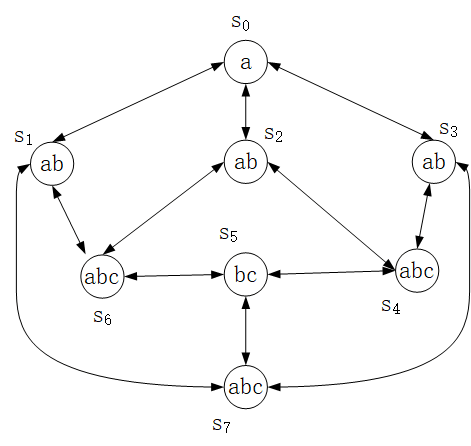
\includegraphics[width=0.4\textwidth]{k2.png}}
        \hspace{1in}
        \subfigure[$V$-quotient Kripke structure of $\Hm$]{
        \label{Kripke_2:VQ} %% label for second subfigure%
       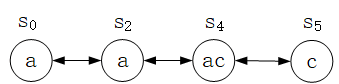
\includegraphics[width=0.3\textwidth]{k2VQ.png}}
       \caption{Computing the $V$-quotient Kripke structure}
    \label{fig:subfig} %% label for entire figure%
\end{figure}
\end{example}



Intuitively, if two Kripke structures are $V$-bisimular, then they satisfy the same formula $\varphi$ that dose not contain any atoms in $V$, \ie\ $\IR(\varphi, V)$.
\begin{theorem}\label{thm:V-bisimulation:EQ}
  Let $V\subseteq\cal A$, ${\cal K}_i~(i=1,2)$ be two Kripke structures such that
  ${\cal K}_1\lrto_V{\cal K}_2$ and $\phi$ a formula with $\IR(\phi,V)$. Then
  ${\cal K}_1\models\phi$ if and only if ${\cal K}_2\models\phi$.
\end{theorem}
%\begin{proof}
%
%\end{proof}

Let $V\subseteq\cal A$, ${\cal M}_i=(S_i,R_i,L_i)~(i=1,2)$ be transition systems.
A computation tree $\Tr_n(s_1)$ of ${\cal M}_1$ is $V$-{\em bisimular}
to a computation tree $\Tr_n(s_2)$ of ${\cal M}_2$, written
$({\cal M}_1,\Tr_n(s_1))\lrto_V({\cal M}_2,\Tr_n(s_2))$ (or simply
$\Tr_n(s_1)\lrto_V\Tr_n(s_2)$), if % $({\cal M}_1,s_1)\lrto_V({\cal M}_2,s_2)$.
\begin{itemize}
  \item $L_1(s_1)-V=L_2(s_2)-V$,
  \item for every subtree $\Tr_{n-1}(s_1')$ of $\Tr_n(s_1)$,
  $\Tr_n(s_2)$ has a subtree $\Tr_{n-1}(s_2')$ such that
  $\Tr_{n-1}(s_1')\lrto_V\Tr_{n-1}(s_2')$, and
  \item for every subtree $\Tr_{n-1}(s_2')$ of $\Tr_n(s_2)$,
  $\Tr_n(s_1)$ has a subtree $\Tr_{n-1}(s_1')$ such that
  $\Tr_{n-1}(s_1')\lrto_V\Tr_{n-1}(s_2')$.
\end{itemize}
Please note that the last two conditions in the above definition
hold trivially for $n=0$.

\begin{proposition}\label{B_to_T}
  Let $V\subseteq\cal A$ and $({\cal M}_i,s_i)~(i=1,2)$ be two Kripke structures.
  Then
  \[(s_1,s_2)\in{\cal B}_n\mbox{ if and only if }
  \Tr_j(s_1)\lrto_V\Tr_j(s_2)\mbox{ for every $0\le j\le n$}.\]
\end{proposition}
%\begin{proof}
%We will prove this from two aspects:
%
%$(\Rto)$ If $s \Hb_n s'$, then $Tr_j(s) \lrto_V Tr_j(s')$ for all $0 \leq j \leq n$. $s \Hb_n s'$ implies both roots of $Tr_n(s)$ and $Tr_n(s')$ have the same atoms except those atoms in $V$.
%Besides, for any $s_1$ with $s\rto s_1$, there is a $s_1'$ with $s'\rto s_1'$ \st $s_1 \Hb_{n-1} s_1'$ and vice versa.
%Then we have $Tr_1(s) \lrto_V Tr_1(s')$.
%Therefore,  $Tr_n(s) \lrto_V Tr_n(s')$ by use such method recursively, and then $Tr_j(s) \lrto_V Tr_j(s')$ for all $0 \leq j \leq n$.
%%It is easy to prove this by the definition of
%
%$(\Lto)$ If $Tr_j(s) \lrto_V Tr_j(s')$ for all $j \leq n$, then $s \Hb_n s'$.
%$Tr_0(s) \lrto_V Tr_0(s')$ implies $L(s) - V = L'(s') - V$ and then $s \Hb_0 s'$.
%$Tr_1(s) \lrto_V Tr_1(s')$ implies $L(s) - V = L'(s')- V$ and for every successors $s_1$ of the root of one, it is possible to find a successor of the root of the other $s_1'$ such that
%$s_1 \Hb_0 s_1'$. Therefore $s \Hb_1 s'$, and then we will have $s \Hb_n s'$ by use such method recursively.
%\end{proof}
This means that $\Tr_j(s_1) \lrto_V \Tr_j(s_2)$ for all $j \geq 0$ if $s_1 \lrto_V s_2$, otherwise there is some number $k$ such that $\Tr_k(s_1)$ and $\Tr_k(s_2)$ are not $V$-bisimular.

\begin{proposition}
  Let $V\subseteq \Ha$, $\Hm =(S,R,L)$ be a transition system and $s,s'\in S$
  such that $(s,s')\notin \cal B$.
  There exists a least number $k$ such that
  $\Tr_k(s)$ and $\Tr_k(s')$ are not $V$-bisimular.
\end{proposition}
%\begin{proof}
%If $(s,s') \notin \cal B$, then there exists a least constant $k$ such that $(s_i, s_j) \notin \Hb_k$, and then there is a constant m ($m \leq k$) such that $\Tr_m(s_i)$ and $\Tr_m(s_j)$ are not V-corresponding by Proposition~\ref{B_to_T}. Let $c=m$, the lemma is proved.
%\end{proof}
In this case the transition ${\cal M}$ is called $V$-{\em distinguishable} (by
states $s$ and $s'$ at the least depth $k$), which is denoted by $\dis_V({\cal M},s,s',k)$.
It is evident that
$\dis_V({\cal M},s,s',k)$ implies $\dis_V({\cal M},s,s',k')$ whenever $k'\ge k$.
The $V$-{\em characterization number}
of ${\cal M}$, written $ch({\cal M},V)$, is defined as
\[ch({\cal M},V)=
\left\{
  \begin{array}{ll}
    \max\{k\mid s,s'\in S\ \&\ \dis_V({\cal M},s,s',k)\},
    & \hbox{${\cal M}$ is $V$-distinguishable;} \\
    \min\{k\mid {\cal B}_{k}={\cal B}\}, & \hbox{otherwise.}
  \end{array}
\right.
\]



\begin{definition}\label{def:V:char:formula}
Let $V\subseteq \Ha$, $\Hm =(S,R,L)$ be a transition system and $s\in S$.
The {\em characterize formula} of the computation tree $\Tr_n(s)$ on $V$,
written ${\cal F}_V(\Tr_n(s))$, is defined recursively as:
\begin{align*}
  & {\cal F}_V(\Tr_0(s)) = \bigwedge_{p \in V\cap L(s)}p
     \wedge \bigwedge_{q\in V-L(s)} \neg q,\\
  & {\cal F}_V(\Tr_{k+1}(s)) = \left(\bigwedge_{(s,s')\in R}
    \EXIST \NEXT {\cal F}_V(\Tr_k(s'))\right)
    \wedge \ALL \NEXT\left(\bigvee_{(s,s')\in R}
    {\cal F}_V(\Tr_k(s') )\right)
    \wedge {\cal F}_V(\Tr_0(s))
\end{align*}
for $k\ge 0$.
\end{definition}


\begin{lemma}\label{Bn:to:Tn}
Let $V\subseteq \Ha$, $\Hm=(S, R, L)$ and $\Hm'=(S', R', L')$ be two transition systems,
$s\in S$, $s'\in S'$ and $n\ge 0$.
\begin{enumerate}[(i)]
  \item $({\cal M},s)\models{\cal F}_V(\Tr_n(s))$.
  \item If $({\cal M},s)\models{\cal F}_V(\Tr_n(s'))$ then
  $\Tr_n(s) \lrto_{\overline V} \Tr_n(s')$.
\end{enumerate}
\end{lemma}
%\begin{proof}
%(i) Base. It is apparent that $({\cal M},s)\models {\cal F}_V(\Tr_0(s))$.\\
%Step. For $k \geq 0$, supposing the result talked in (i) is correct in $k - 1$, we will show that $({\cal M},s)\models {\cal F}_V(\Tr_{k+1}(s))$, \ie:
% \[({\cal M},s)\models \left(\bigwedge_{(s,s')\in R}
%    \EXIST \NEXT {\cal F}_V(\Tr_k(s'))\right)
%    \wedge \ALL \NEXT\left(\bigvee_{(s,s')\in R}
%    {\cal F}_V(\Tr_k(s') )\right)
%    \wedge {\cal F}_V(\Tr_0(s)).\]
%It is apparent that $({\cal M},s)\models {\cal F}_V(\Tr_0(s))$ by Base. It is apparent that for any $(s,s') \in R$, there is $({\cal M}, s') \models {\cal F}_V(\Tr_k(s'))$ by inductive assumption. Then we have $({\cal M},s)\models \EXIST \NEXT {\cal F}_V(\Tr_k(s')$, and then $({\cal M},s)\models \left(\bigwedge_{(s,s')\in R}
%    \EXIST \NEXT {\cal F}_V(\Tr_k(s'))\right)$. Similarly, we have that for any $(s,s') \in R$, there is $({\cal M}, s') \models \bigvee_{(s,s'')\in R}
%    {\cal F}_V(\Tr_k(s'') )$. Therefore, $({\cal M},s)\models \ALL \NEXT\left(\bigvee_{(s,s'')\in R}
%    {\cal F}_V(\Tr_k(s'') )\right)$.
%
%(ii)  \textbf{Base}. If $n=0$, then $(\Hm, s)  \models {\cal F}_V(\Tr_0(s'))$ implies $L(s) - \overline V = L'(s') - \overline V$. Hence, $\Tr_0(s) \lrto_{\overline V} \Tr_0(s')$.\\
%    \textbf{Step}. Supposing $n>0$ and the result talked in (ii) is correct in $n-1$.\\
%   (a) It is easy to see that $L(s) - \overline V = L'(s') - \overline V$.\\
%   (b) We will show that for each $(s, s_1) \in R$, there is a $(s', s_1') \in R'$ such that $\Tr_{n-1}(s_1) \lrto_{\overline V} \Tr_{n-1}(s_1')$.
%      Since $(\Hm, s) \models {\cal F}_V(\Tr_n(s'))$, then $(\Hm, s) \models \ALL \NEXT\left(\bigvee_{(s',s_1')\in R}{\cal F}_V(\Tr_{n-1}(s_1') )\right)$.
%      Therefore, for each $(s, s_1) \in R$ there is a $(s', s_1') \in R'$ such that $(\Hm, s_1) \models {\cal F}_V(\Tr_{n-1}(s_1') )$. Hence, $\Tr_{n-1}(s_1) \lrto_{\overline V} \Tr_{n-1}(s_1')$ by inductive hypothesis.\\
%   (c) We will show that for each $(s',s_1')\in R'$ there is a $(s,s_1)\in R$ such that $\Tr_{n-1}(s_1') \lrto_{\overline V} \Tr_{n-1}(s_1)$.
%      Since $(\Hm, s) \models {\cal F}_V(\Tr_n(s'))$, then $(\Hm, s) \models  \bigwedge_{(s',s_1')} \EXIST \NEXT {\cal F}_V(\Tr_{n-1}(s_1'))$.
%      Therefore, for each $(s',s_1')\in R'$ there is a $(s,s_1)\in R$ such that $(\Hm, s_1) \models {\cal F}_V(\Tr_{n-1}(s_1')$.
%      Hence, $\Tr_{n-1}(s_1) \lrto_{\overline V} \Tr_{n-1}(s_1')$ by inductive hypothesis.
%\end{proof}


A consequence of the previous lemma is:

\begin{lemma}\label{div_s}
Let $V\subseteq \Ha$, $\Hm=(S,R,L)$ a transition system, $k={ch({\cal M},V)}$ and $s\in S$.
%There is a formula $\phi$ such that
\begin{itemize}
  \item $(\Hm, s)\models {\cal F}_V(\Tr_k(s))$, and
  \item for each $s'\in S$, $({\cal M},s) \lrto_{\overline V} ({\cal M},s')$
  if and only if $({\cal M},s')\models{\cal F}_V(\Tr_k(s))$.
\end{itemize}
\end{lemma}
\begin{proof}
Let $\phi = {\cal F}_V(\Tr_k(s))$, where $c$ is the V-characteristic number of $\Hm$. $\Hm, s \models \phi$ by the definition of ${\cal F}$, and then $\forall s' \in S$, if $s \lrto_{\overline V} s'$ there is $\Hm, s' \models \phi$ by Theorem~\ref{thm:V-bisimulation:EQ} due to $\IR(\phi, \Ha \setminus V)$. If $s \nleftrightarrow_{\overline V} s'$, then $\Tr_c(s) \not \lrto_{\overline V} \Tr_c(s')$, and then $\Hm, s\nvDash \phi$ by Lemma~\ref{Bn:to:Tn}.
\end{proof}


Let $V\subseteq\cal A$, ${\cal M}=(S,R,L)$
and ${\cal K}=({\cal M},s_0)$ be an initial Kripke structure.
The {\em characterizing formula} of $\cal K$ on $V$, written ${\cal F}_V(\Hm,s_0)$ (or ${\cal F}_V({\cal K})$), is
defined as the conjunction of the following formulas:
\begin{align*}
  &{\cal F}_V(\Tr_c(s_0)), \mbox{ and }\\
%  &  \bigwedge_{s\in S}\left(
  & \ALL \GLOBAL\left(
    {\cal F}_V(\Tr_c(s)) \rto
    \bigwedge_{(s,s')\in R}
        \EXIST \NEXT {\cal F}_V(\Tr_c(s'))
        \wedge
        \ALL \NEXT \bigvee_{(s,s')\in R}{\cal F}_V(\Tr_c(s'))
    \right), \ s\in S
\end{align*}
where $c=ch({\cal M},V)$. It is apparent that $\IR({\cal F}_V(\Hm, s_0), \overline V)$.


\begin{lemma}\label{lem:models:formula}
  Let $\varphi$ be a formula. We have
  \begin{equation}
    \varphi\equiv \bigvee_{(\Hm, s_0)\in\Mod(\varphi)}{\cal F}_{\cal A}(\Hm, s_0).
\end{equation}
\end{lemma}
%lem:models:formula\begin{proof}
%Let $(\Hm', s_0')$ be a model of $\varphi$. Then $(\Hm', s_0') \models \bigvee_{(\Hm, s_0)\in \Mod(\varphi)} {\cal F}_{\Ha}(\Hm, s_0)$ due to $(\Hm', s_0') \models {\cal F}_{\Ha}(\Hm', s_0')$. On the other hand, suppose that $(\Hm', s_0')$ is a model of $\bigvee_{(\Hm, s_0)\in \Mod(\varphi)} {\cal F}_{\Ha}(\Hm, s_0)$. Then there is a $(\Hm, s_0)\in \Mod(\varphi)$ such that $(\Hm', s_0') \models {\cal F}_{\Ha}(\Hm, s_0)$. And then $(\Hm, s_0) \lrto_{\O} (\Hm', s_0')$ by Theorem~\ref{CF}. Therefore, $(\Hm, s_0)$ is also a model of $\varphi$ by Theorem~\ref{thm:V-bisimulation:EQ}.
%\end{proof}
This means that any CTL formula can be described by the disjunction of the characterizing formulas of all the models of itself due to the number of modes of a CTL formula is finite.

\begin{theorem}\label{CF}
Let $V\subseteq \Ha$, $\Hm=(S,R,L)$ a transition system with initial state $s_0$
and $\Hm'=(S',R', L')$ a transition system with initial state $s_0'$.
Then  $$(\Hm',s_0') \models {\cal F}_V({\cal M},s_0)
\mbox{ if and only if }
({\cal M},s_0) \lrto_{\overline V} ({\cal M}',s_0').$$
\end{theorem}
%\begin{proof}
%%Let $\Hm_u = (S_u, R_u, L_u)$ a transition system with initial state $s_u$, where $S_u=S\cup S' \cup \{s_u\}$, $R_u = R \cup R' \cup \{(s_u, s_0), (s_u, s_0')\}$ and $L_u: S_u \rto 2^{\Ha}$ is defined as:
%%\[L_u(s)=
%%\left\{
%%  \begin{array}{ll}
%%    L(s), & \hbox{if $s\in S$,} \\
%%    L'(s), & \hbox{if $s\in S'$,}\\
%%    ${\O}$, & \hbox{$s=s_u$}.
%%  \end{array}
%%\right.
%%\]
%%%It is apparent that $\forall s \in (S\cup S')$, $s_u \not \lrto_{\overline V} s$.
%%
%%Let ${\cal F}_V(\Hm, s_0) = {\cal F}_V(\Tr_c(s_0)) \wedge \bigwedge_{s\in S} G(\Hm, s)$, where:
%%\[
%%  G(\Hm, s) = \ALL \GLOBAL \left({\cal F}_V(\Tr_c(s)) \rto \left(\bigwedge_{(s,s_1)\in R} \EXIST \NEXT {\cal F}_V(\Tr_c(s_1)) \right) \wedge \ALL \NEXT \left(\bigvee_{(s,s_1)\in R} {\cal F}_V(\Tr_c(s_1)) \right) \right)
%%      \] and $c=ch(\Hm_u, V)$.\\
%
%Let ${\cal F}_V(\Hm, s_0)$ be the characterizing formula of $(\Hm, s_0)$ on $V$.
%It is apparent that $\IR({\cal F}_V(\Hm, s_0), \overline V)$. We will show that $\Hm, s_0 \models {\cal F}_V(\Hm, s_0)$ at first.
%
%It is apparent that $(\Hm, s_0) \models {\cal F}_V(\Tr_c(s_0))$ by Lemma~\ref{Bn:to:Tn}.
%We must show that $\Hm, s_0 \models \bigwedge_{s\in S} G(\Hm, s)$.
%Let ${\cal X} = {\cal F}_V(\Tr_c(s)) \rto \left(\bigwedge_{(s,s_1) \in R} \EXIST \NEXT {\cal F}_V(\Tr_c(s_1))\right)$ $\wedge \ALL \NEXT \left(\bigvee_{(s,s_1) \in R} {\cal F}_V(\Tr_c(s_1))\right)$, we will show $\forall s\in S$, $\Hm, s_0 \models G(\Hm, s)$.
%%Let $s_1, s_2, ..., s_m$ be the successors of $s$.
%There are two cases we should consider:
%\begin{itemize}
%  \item  If $\Hm, s_0 \nvDash {\cal F}_V(\Tr_c(s))$, it is apparent that $\Hm, s_0 \models {\cal X}$;
%  \item  If $\Hm, s_0 \models {\cal F}_V(\Tr_c(s))$:\\
%         $\Hm, s_0 \models {\cal F}_V(\Tr_c(s))$\\
%        $\Rto$  $s_0 \lrto_{\overline V} s$ by the definition of characteristic number and Lemma~\ref{div_s}\\
%        for each $(s, s_1)\in R$ there is $(\Hm, s_1) \models {\cal F}_V(\Tr_c(s_1))$  \hfill  ($s_1 \lrto_{\overline V} s_1$)\\
%        $\Rto$ $(\Hm, s) \models \bigwedge_{(s,s_1)\in R}\EXIST \NEXT {\cal F}_V(\Tr_c(s_1))$\\
%        $\Rto$ $(\Hm, s_0) \models \bigwedge_{(s,s_1)\in R}\EXIST \NEXT {\cal F}_V(\Tr_c(s_1))$     \hfill   ($\IR(\bigwedge_{(s,s_1)\in R}\EXIST \NEXT {\cal F}_V(\Tr_c(s_1)), \overline V)$, $s_0 \lrto_{\overline V} s$)\\
%         for each $(s, s_1)$ there is $\Hm, s_1 \models \bigvee_{(s, s_2)\in R}{\cal F}_V(\Tr_c(s_2))$\\
%        $\Rto$ $(\Hm, s) \models \ALL \NEXT \left( \bigvee_{(s, s_2)} {\cal F}_V(\Tr_c(s_2)) \right)$ \\
%        $\Rto$ $(\Hm, s_0) \models  \ALL \NEXT \left( \bigvee_{(s, s_2)} {\cal F}_V(\Tr_c(s_2)) \right)$   \hfill  ($\IR(\ALL \NEXT \left( \bigvee_{(s, s_2)} {\cal F}_V(\Tr_c(s_2)) \right), \overline V)$, $s_0 \lrto_{\overline V} s$)\\
%        $\Rto$ $(\Hm, s_0) \models {\cal X}$.\\
%       % where $s_i$ and $s_j$ are the successors of $s$.
%\end{itemize}
%%For any other states which can reach from $s_0$ can be proved similarly.
%Therefore, $\forall s\in S$, $(\Hm, s_0) \models G(\Hm, s)$, and then $(\Hm, s_0) \models {\cal F}_V(\Hm, s_0)$.
%
%
%We will prove this theorem from the following two aspects:
%
%$(\Lto)$ If $s_0 \lrto_{\overline V} s_0'$, then $\Hm',s_0' \models {\cal F}_V(M,s_0)$. Since $\Hm, s_0 \models {\cal F}_V(\Hm, s_0)$ and $\IR({\cal F}_V(\Hm, s_0), \overline V)$, hence
%$\Hm',s_0' \models {\cal F}_V(M,s_0)$ by Theorem~\ref{thm:V-bisimulation:EQ}.
%
%$(\Rto)$ If $\Hm',s_0' \models {\cal F}_V(M,s_0)$, then $s_0 \lrto_{\overline V} s_0'$. We will prove this by showing that $\forall n \geq 0$, $Tr_n(s_0) \lrto_{\overline V} Tr_n(s_0')$.
%
%%that $\forall n \geq 0$, $\Tr_n(s_0) \lrto_{\overline V} \Tr_n(s_0')$.\\
% %(i) It is apparent that $(s_0, s_0')\in \Hb_0$.
%\textbf{Base}. It is apparent that $Tr_0(s_0) \equiv Tr_0(s_0')$.
%
%\textbf{Step}. Supposing $\Tr_k(s_0) \lrto_{\overline V} \Tr_k(s_0')$ ($k > 0$), we will prove $\Tr_{k+1}(s_0) \lrto_{\overline V} \Tr_{k+1}(s_0')$. We should only show that $\Tr_1(s_k) \lrto_{\overline V} \Tr_1(s_k')$. Where $(s_0, s_1), (s_1, s_2)$, $\dots$, $(s_{k-1}, s_k) \in R$ and $(s_0', s_1'), (s_1', s_2'), \dots, (s_{k-1}', s_k') \in R'$.
% % Let $s_{i,x}$ be a node in depth $i$ in $Tr_{k+1}(s_0)$ and $s_{i+1,x_1}, s_{i+1,x_2}, ..., s_{i+1,x_m}$ be the successors of $s_{i,x}$. By $s_{i+1,x_j}$ we mean the $j$th successor of $s_{i, x}$ ($i \geq 0$, $j\in \{1,2,...,m\}$ and $x$ is a constant), $s_{0,0}=s_0$.
%%      Let $0_{i^2} = 0_{i_i}$, $0_{i^3}= 0_{i_{i_i}}$ and so on.
%%      For $Tr_{k+1}(s_0')$, we plus a prime for those tokens. We should only show that for any $s_{k, i}$ there is a $s_{k,j}'$ such that $Tr_1(s_{k, i})\equiv_{\Ha \setminus V} Tr_1(s_{k, j}')$, and for any $s_{k, j}'$ there is a $s_{k,i}$ such that $Tr_1(s_{k, i})\equiv_{\Ha \setminus V} Tr_1(s_{k, j}')$ by induction hypothesis.
%
%      (i) It is apparent that $L(s_k) - \overline V = L'(s_k') - \overline V$ by inductive assumption.
%
%      Before talking about the other points, note the following fact that:\\
%      $(\Hm',s_0') \models {\cal F}_V(\Hm,s_0)$\\
%      $\Rto$ $\forall s'\in S'$, $(\Hm', s') \models {\cal F}_V(\Tr_c(s)) \rto \left(\bigwedge_{(s,s_1)\in R} \EXIST \NEXT {\cal F}_V(\Tr_c(s_1))\right) \wedge \ALL \NEXT \left( \bigvee_{(s,s_1)\in R} {\cal F}_V(\Tr_c(s_1))\right)$ for any $s\in S$.   \hfill  \textbf{(fact)}\\
%      (I) $(\Hm', s_0') \models {\cal F}_V(\Tr_c(s_0)) \rto \left(\bigwedge_{(s_0, s_1) \in R} \EXIST \NEXT {\cal F}_V(\Tr_c(s_1))\right)$ $\wedge$ $\ALL \NEXT \left(\bigvee_{(s_0, s_1) \in R} {\cal F}_V(\Tr_c(s_1)) \right)$     \hfill  \textbf{(fact)}\\
%        (II) $(\Hm', s_0') \models {\cal F}_V(\Tr_c(s_0)))$  \hfill  (known)\\
%        (III) $(\Hm', s_0') \models \left(\bigwedge_{(s_0, s_1) \in R} \EXIST \NEXT {\cal F}_V(\Tr_c(s_1))\right)$ $\wedge$ $\ALL \NEXT \left(\bigvee_{(s_0, s_1) \in R} {\cal F}_V(\Tr_c(s_1)) \right)$  \hfill  ((I),(II))\\
%
%      % It is apparent that $L'(s_0') - \overline V = L(s_0) - \overline V$;\\
%        (ii) We will show that for each $(s_k, s_{k+1}) \in R$ there is a $(s_k', s_{k+1}') \in R'$ such that $L(s_{k+1}) - \overline V = L'(s_{k+1}') - \overline V$.\\
%        (1) $(\Hm', s_0') \models \bigwedge_{(s_0, s_1) \in R} \EXIST \NEXT {\cal F}_V(\Tr_c(s_1))$  \hfill  (III)\\
%        (2) $\forall (s_0, s_1) \in R$, $\exists (s_0', s_1') \in R'$ \st\ $(\Hm', s_1') \models {\cal F}_V(\Tr_c(s_1))$  \hfill  (2)\\
%        (3) $\Tr_c(s_1) \lrto_{\overline V} \Tr_c(s_1')$  \hfill  ((2), Lemma~\ref{Bn:to:Tn}) \\
%        (4) $L(s_1) - \overline V = L'(s_1') - \overline V$  \hfill   ((3), $c \geq 0)$\\
%        (5) $(\Hm', s_1') \models {\cal F}_V(\Tr_c(s_1)) \rto \left(\bigwedge_{(s_1,s_2)\in R} \EXIST \NEXT {\cal F}_V(\Tr_c(s_2))\right) \wedge \ALL \NEXT \left(\bigvee_{(s_1,s_2)\in R} {\cal F}_V(\Tr_c(s_2))\right)$     \hfill  \textbf{(fact)}\\
%        (6) $(\Hm', s_1') \models \left(\bigwedge_{(s_1,s_2)\in R} \EXIST \NEXT {\cal F}_V(\Tr_c(s_2))\right) \wedge \ALL \NEXT \left(\bigvee_{(s_1,s_2)\in R} {\cal F}_V(\Tr_c(s_2))\right)$ \hfill ((2), (5))\\
%        (7) $\dots \dots$ \\
%        (8) $(\Hm', s_k') \models \left(\bigwedge_{(s_k,s_{k+1})\in R} \EXIST \NEXT {\cal F}_V(\Tr_c(s_{k+1}))\right) \wedge \ALL \NEXT \left(\bigvee_{(s_k,s_{k+1})\in R} {\cal F}_V(\Tr_c(s_{k+1}))\right)$       \hfill (similar with (6))\\
%        (9) $\forall (s_k, s_{k+1}) \in R$, $\exists (s_k', s_{k+1}') \in R'$ \st\ $(\Hm', s_{k+1}') \models {\cal F}_V(\Tr_c(s_{k+1}))$  \hfill  (8)\\
%        (10) $\Tr_c(s_{k+1}) \lrto_{\overline V} \Tr_c(s_{k+1}')$    \hfill ((9), Lemma~\ref{Bn:to:Tn}) \\
%        (11) $L(s_{k+1}) - \overline V = L'(s_{k+1}') - \overline V$  \hfill   ((10), $c \geq 0)$\\
%
%       % (3) $s_1 \lrto_{\overline V} s_1'$   \hfill  ((2), Lemma~\ref{div_s})
%
%        %(3) $\Tr_c(s_1) \lrto_{\overline V} \Tr_c(s_1')$  \hfill  ((2), Lemma~\ref{Bn:to:Tn})\\
%       % (4) $\Tr_k(s_1) \lrto_{\overline V} \Tr_k(s_1')$ \hfill (by the Definition~\ref{def:V-bisimulation})\\
%        (iii) We will show that for each $(s_k', s_{k+1}') \in R'$ there is a $(s_k, s_{k+1})\in R$ such that $L(s_{k+1}) - \overline V = L'(s_{k+1}') - \overline V$.\\
%        (1) $(\Hm', s_k') \models \ALL \NEXT \left(\bigvee_{(s_k,s_{k+1})\in R} {\cal F}_V(\Tr_c(s_{k+1}))\right)$  \hfill (by (8) talked above)\\
%        (2) $\forall (s_k', s_{k+1}') \in R'$, $\exists (s_k, s_{k+1}) \in R$ \st\ $(\Hm', s_{k+1}') \models {\cal F}_V(\Tr_c(s_{k+1}'))$  \hfill (1) \\
%        (3) $\Tr_c(s_{k+1}) \lrto_{\overline V} \Tr_c(s_{k+1}')$    \hfill ((2), Lemma~\ref{Bn:to:Tn}) \\
%        (4) $L(s_{k+1}) - \overline V = L'(s_{k+1}') - \overline V$  \hfill   ((3), $c \geq 0)$\\
%
%        %(1) $(M', s_0') \models \ALL \NEXT \left(\bigvee_{(s_0, s_1) \in R} {\cal F}_V(\Tr_c(s_1)) \right)$  \hfill (III)\\
%%        (2) for each $(s_0', s_1') \in R'$ there is $(\Hm', s_1') \models \bigvee_{(s_0, s_1) \in R} {\cal F}_V(\Tr_c(s_1))$  \hfill (1)\\
%%        (3) there is a $(s_0, s_1) \in R$ such that $(\Hm', s_1') \models {\cal F}_V(\Tr_c(s_1))$  \hfill (2) \\
%%        (4) $s_1 \lrto_{\overline V} s_1'$   \hfill  ((3), Lemma~\ref{div_s})\\
%        %(4) $\Tr_c(s_1) \lrto_V \Tr_c(s_1')$  \hfill  ((2),(3), Lemma~\ref{Bn:to:Tn})\\
%       % (5) $\Tr_k(s_1) \lrto_{\overline V} \Tr_k(s_1')$ \hfill (by the Definition~\ref{def:V-bisimulation})
%
%\end{proof}

We will give an example to show the computing of characterizing formula:
\begin{example}
Let ${\cal K} = (\Hm, s_0)$ with $\Hm=(S, R, L)$ be a initial Kripke structure (in Fig.~\ref{Kripke_1}), in which $S=\{s_0, s_1, s_2\}$, $R=\{(s_0, s_1), (s_0, s_2), (s_1, s_0), (s_2, s_0)\}$, $L(s_0)= \{a\}$, $L(s_1) =\{a,c\}$ and $L(s_2) = \{b,c\}$. Let $V=\{a, b\}$, compute the characterizing formula of ${\cal K}$ on $V$.

It is apparent that $\Tr_0(s_0) \lrto_{\overline V} \Tr_0(s_1)$ due to $L(s_0) - \overline V = L(s_1) -\overline V$, $\Tr_1(s_0) \not\lrto_{\overline V} \Tr_1(s_1)$ due to there is $(s_0, s_2)\in R$ such that for any $(s_1, s') \in R$ (there is only one immediate successor $s'=s_0$) there is $L(s_2) - \overline V \neq L(s') - \overline V$. Hence, we have that $\Hm$ is $\overline V$-distinguished by state $s_0$ and $s_1$ at the least depth 1, \ie\ $\dis_{\overline V}(\Hm, s_0, s_1, 1)$. Similarly, we have $\dis_{\overline V}(\Hm, s_0, s_2, 0)$ and $\dis_{\overline V}(\Hm, s_1, s_2, 0)$. Therefore, $ch(\Hm, \overline V) =  \max\{k\mid s,s'\in S\ \&\ \dis_{\overline V}({\cal M},s,s',k)\} = 1$.
%It is apparent that $\Hb_0=\{(s_0, s_1)\}$ and $\Hb_1={\O}$, then $ch(\Hm, s_0) = 1$.
Then we have:
\begin{align*}
  & {\cal F}_V(\Tr_0(s_0)) = a \wedge \neg b, \\
  & {\cal F}_V(\Tr_0(s_1)) = a \wedge \neg b, \\
  & {\cal F}_V(\Tr_0(s_2)) = b \wedge \neg a, \\
  & {\cal F}_V(\Tr_1(s_0)) = \EXIST\NEXT(a \wedge \neg b)  \wedge \EXIST\NEXT(b \wedge \neg a) \wedge \ALL\NEXT((a \wedge \neg b) \vee (b \wedge \neg a)) \wedge (a \wedge \neg b), \\
  & {\cal F}_V(\Tr_1(s_1)) = \EXIST\NEXT(a \wedge \neg b)  \wedge \ALL\NEXT(a \wedge \neg b) \wedge (a \wedge \neg b), \\
  & {\cal F}_V(\Tr_1(s_2)) = \EXIST\NEXT(a \wedge \neg b)  \wedge \ALL\NEXT(a \wedge \neg b) \wedge (b \wedge \neg a).\\
  & \mbox{ Then it is easy to obtain\ } {\cal F}_V(\Hm, s_0).
  %&{\cal F}_V(\Hm, s_0)= {\cal F}_V(\Tr_1(s_0)) \wedge  \bigwedge_{s\in S} \ALL \GLOBAL \left(
%  {\cal F}_V(\Tr_1(s)) \rto
%  \bigwedge_{(s,s')\in R}
%        \EXIST \NEXT {\cal F}_V(\Tr_1(s'))
%        \wedge
%        \ALL \NEXT \bigvee_{(s,s')\in R}{\cal F}_V(\Tr_1(s'))
%  \right)
\end{align*}

\begin{figure}
  \centering
  % Requires \usepackage{graphicx}
  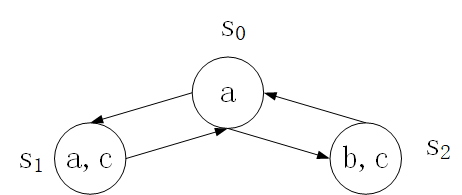
\includegraphics[width=5cm]{k1.png}\\
  \caption{A simple Kripke structure}\label{Kripke_1}
\end{figure}
\end{example}



\subsection{Forgetting}

Having talked about the $V$-bisimulation between two Kripke structures and the characterizing formula of a Kripke structure, we will give the definition of forgetting under CTL from the sematic forgetting point of view.
\begin{definition}[Forgetting]\label{def:V:forgetting}
  Let $V\subseteq\cal A$ and $\phi$ a formula.
A formula $\psi$ with $\Var(\psi)\cap V=\emptyset$
is a {\em result of forgetting $V$ from} $\phi$, if
\begin{equation}
  \Mod(\psi)=\{{\cal K}\mbox{ is initial}\mid \exists {\cal K}'\in\Mod(\phi)\ \&\ {\cal K}'\lrto_V{\cal K}\}.
\end{equation}
\end{definition}
Note that if both $\psi$ and $\psi'$ are results of forgetting $V$ from $\phi$ then
$\Mod(\psi)=\Mod(\psi')$, \ie, $\psi$ and $\psi'$ have the same models. In the sense
of equivalence the forgetting result is unique (up to equivalence).
By Lemma~\ref{lem:models:formula}, such a formula $\psi$ always exists, which
is equivalent to
\begin{equation*}
  \bigvee_{{\cal K}\in  \{{\cal K}'\mbox{ is an initial interpretation}\mid \exists {\cal K}''\in\Mod(\phi)\ \&\ {\cal K}''\lrto_V{\cal K}'\}} {\cal F}_{\overline V}({\cal K}).
\end{equation*}
For this reason, the forgetting result is denoted by $\CTLforget(\phi,V)$.

In the case $\psi$ is a result of forgetting $V$ from $\phi$, there are usually some
expected properties (called {\em postulates}) for them~\cite{Yan:AIJ:2009}:
\begin{itemize}
  \item Weakening (\W): $\varphi \models \psi$;
  \item Positive Persistence (\PP):
    if $\IR(\eta, V)$ and $\varphi \models \eta$, then $\psi \models \eta$;
  \item Negative Persistence (\NgP): if $\IR(\eta, V)$ and $\varphi \nvDash \eta$, then $\psi \nvDash \eta$;
  \item Irrelevance (\textbf{IR}): $\IR(\psi, V)$.
\end{itemize}



\begin{theorem}\label{thm:close}
Let $\varphi$ and $\psi$ be two formulas and $V \subseteq \Ha$.
Then the following statements are equivalent:
\begin{enumerate}[(i)]
  \item $\psi \equiv \CTLforget(\varphi, V)$,
  \item $\psi \equiv \{\phi | \varphi \models \phi \& \IR(\phi, V)\}$,
  \item Postulates (\W), (\PP), (\NgP) and (\textbf{IR}) hold.
\end{enumerate}
\end{theorem}
We can see from this theorem that the forgetting under CTL is closed, \ie\ for any CTL formula the result of forgetting is also a CTL formula.
%\begin{proof}
%$(i) \LRto (ii)$. To prove this, we will show that:
%\[
%\Mod(\CTLforget(\varphi, V)) = \Mod(\{\phi | \varphi \models \phi, \IR(\phi, V)\}) = \Mod(\bigvee_{\Hm, s_0\in \Mod(\varphi)} {\cal F}_{\Ha\setminus V}(\Hm, s_0)).
%\]
%Firstly, suppose that $(\Hm', s_0')$ is a model of $\CTLforget(\varphi, V)$. Then there exists an  an initial Kripke structure $(\Hm, s_0)$ such that $(\Hm, s_0)$ is a model of $\varphi$ and $(\Hm, s_0) \lrto_V (\Hm', s_0')$. By Theorem~\ref{thm:V-bisimulation:EQ}, we have $(\Hm', s_0') \models \phi$ for all $\phi$ that $\varphi\models \phi$ and $\IR(\phi, V)$. Thus, $(\Hm', s_0')$ is a model of $\{\phi | \varphi \models \phi, \IR(\phi, V)\}$.
%
%Secondly, suppose that $(\Hm', s_0')$ is a models of $\{\phi | \varphi \models \phi, \IR(\phi, V)\}$. Thus, $(\Hm', s_0')$ $\models$ $\bigvee_{(\Hm, s_0)\in \Mod(\varphi)} {\cal F}_{\Ha\setminus V}(\Hm, s_0)$ due to $\bigvee_{(\Hm, s_0)\in \Mod(\varphi)} {\cal F}_{\Ha\setminus V}(\Hm, s_0)$ is irrelevant to $V$.
%
%Finally, suppose that $(\Hm', s_0')$ is a model of $\bigvee_{\Hm, s_0\in \Mod(\varphi)} {\cal F}_{\Ha\setminus V}(\Hm, s_0)$. Then there exists $(\Hm, s_0) \in \Mod(\varphi)$ such that $(\Hm', s_0') \models {\cal F}_{\Ha\setminus V}(\Hm, s_0)$. Hence, $(\Hm, s_0)$ $\lrto_V$ $(\Hm', s_0')$ by Theorem~\ref{CF}. Thus $(\Hm', s_0')$ is also a model of $\CTLforget(\varphi,V)$.
%
%
%$(ii)\Rto (iii)$. It is not difficult to prove it.
%
%$(iii)\Rto (ii)$. Suppose that all postulates hold. By Positive Persistence, we have $\psi \models \{\phi | \varphi \models \phi, \IR(\phi, V)\}$. Now
%we show that $\{\phi | \varphi \models \phi, \IR(\phi, V)\} \models \psi$. Otherwise, there exists formula $\phi'$ such that $\psi \models \phi'$ but $\{\phi | \varphi \models \phi, \IR(\phi, V)\} \nvDash \phi'$. There are three cases:
%\begin{itemize}
%  \item $\phi'$ is relevant to $V$. Thus, $\psi$ is also relevant to $V$, a contradiction to Irrelevance.
%  \item $\phi'$ is irrelevant to $V$ and $\varphi \models \phi'$. This contradicts to our assumption.
%  \item $\phi'$ is irrelevant to $V$ and $\varphi \nvDash \phi'$. By Negative Persistence, $\psi \nvDash \phi'$, a contradiction.
%\end{itemize}
%Thus, $\psi$ is equivalent to $\{\phi | \varphi \models \phi, \IR(\phi, V)\}$.
%\end{proof}


\begin{lemma}\label{lem:KF:eq}
	Let $\varphi$ and $\alpha$ be two \CTL\ formulae and $q\in
		\overline{\Var(\varphi\cup\{\alpha\})}$. Then
	$\forget(\varphi \cup\{q\lrto\alpha\}, q)\equiv \varphi$.
\end{lemma}
%lem:KF:eq\begin{proof}
%	Let $\varphi' =\varphi \cup\{q\lrto\alpha\}$. For any T-model ${\cal M},s$ of $\forget(\Gamma', q)$ there is an I-structure $({\cal M}',s')$ \st\ $({\cal M},s)\lrto_{\{q\}}({\cal M}',s')$ and $({\cal M}',s') \models \varphi'$. It's apparent that $({\cal M}',s') \models \varphi$, and then $({\cal M},s) \models \varphi$ since $IR(\varphi,\{q\})$ and $({\cal M},s)\lrto_{\{q\}}({\cal M}',s')$
%	by Theorem~\ref{IR_EM}.
%
%	Let $(\Hm,s) \in \Mod(\varphi)$ with ${\cal M}=(S, R, L)$. We construct $(\Hm', s)$ with $\Hm' = (S, R, L')$ as follows:
%    \begin{align*}
%       & L':S \rto \Ha\ and\ \forall s^*\in S, L'(s^*) = L(s^*)\ if\ (\Hm, s^*) \nvDash \alpha,\ else\ L'(s^*) = L(s^*)\cup\{q\}, \\
%       & L'(s) = L(s) \cup\{q\}\ if\ (\Hm, s) \models \alpha,\ and\ L'(s^*) = L(s^*)\ otherwise.
%    \end{align*}
%	It is clear that $({\cal M}',s) \models \varphi$, $({\cal M}',s) \models q\lrto \alpha$ and
%	$({\cal M}', s) \lrto_{\{q\}} ({\cal M}, s)$. Therefore $({\cal M}', s) \models \varphi \cup\{q\lrto \alpha\}$, and then $({\cal M}, s) \models \forget (\varphi \cup\{q\lrto\alpha\}, q)$ by
%	$({\cal M}', s) \lrto_{\{q\}} ({\cal M}, s)$.
%\end{proof}


\begin{proposition}\label{disTF}
Let $\varphi$ be a formula, $V$ a set of atoms and $p$ an atom such that $p \notin V$. Then:
\[
\CTLforget(\varphi, \{p\} \cup V) \equiv \CTLforget(\CTLforget(\varphi, p), V).
\]
\end{proposition}
This means that the result of forgetting $V$ from $\varphi$ can be obtained by forgetting atom in $V$ one by one.
Similarly, a consequence of the previous proposition is:
%\begin{proof}
%Let $(\Hm_1, s_1) $ with ${\cal M}_1=(S_1, R_1, L_1)$ be a model of $\CTLforget(\varphi, \{p\} \cup V)$. By the definition, there exists a model $(\Hm,s)$ with ${\cal M} = (S, R,L)$ of $\varphi$, such that $(\Hm_1, s_1)$ $\lrto_{\{p\} \cup V}$ $(\Hm, s)$ via a binary relation $\Hb$. We construct an initial Kripke structure $(\Hm_2, s_2)$ with ${\cal M}_2 = (S_2, R_2, L_2)$ as follows:
%\begin{enumerate}[(1)]
%  \item for $s_2$: let $s_2$ be the state such that:
%  \begin{itemize}
%    \item $p \in L_2(s_2)$ iff $p \in L_1(s_1)$,
%    \item for all $q \in V$, $q \in L_2(s_2)$ iff $q\in L(s)$,
%    \item for all other atoms $q'$, $q' \in L_2(s_2)$ iff $q' \in L_1(s_1)$ iff $q'\in L(s)$.
%  \end{itemize}
%  \item for another:
%  \begin{enumerate}[(i)]
%    \item for all pairs  $w \in S$ and $w_1 \in S_1$ such that $w \Hb w_1$, let $w_2 \in S_2$ and
%        \begin{itemize}
%          \item $p \in L_2(w_2)$ iff $p \in L_1(w_1)$,
%          \item for all $q \in V$, $q \in L_2(w_2)$ iff $q\in L(w)$,
%          \item for all other atoms $q'$, $q' \in L_2(w_2)$ iff $q' \in L_1(w_1)$ iff $q'\in L(w)$.
%        \end{itemize}
%    \item if $w_1' \Hr_1 w_1$, $w_2$ is constructed based on $w_1$ and $w_2'\in S_2$ is constructed based on $w_1'$, then $w_2' \Hr_2 w_2$.
%     %And if $w' \Hr^i w$, $w_2$ is constructed based on $w$ and $w_2'\in \Hw_2$ is constructed based on $w'$, then $w_2' \Hr_2^i w_2$
%    %\item if $\exists w_1'\in \Hw_1$ such that $w_1' \Hr_1 w_1$, then let $w_2' \in \Hw_2$, $w_2' \Hr_2 w_2$, and if $w_1' \neq s_1$ then do (i) for $w_2'$, else let$w_2' = s_2$.
%  \end{enumerate}
%  \item delete duplicated states in $S_2$ and pairs in $R_2$.
%\end{enumerate}
%Then we have $(\Hm, s) \lrto_{\{p\}} (\Hm_2, s_2)$ and $(\Hm_2, s_2) \lrto_V (\Hm_1, s_1)$. Thus, $(\Hm_2, s_2) \models \CTLforget(\varphi, p)$. And therefore $(\Hm_1, s_1) \models \CTLforget(\CTLforget(\varphi, p), V)$.
%
%On the other hand, suppose that $(\Hm_1, s_1)$ be a model of $\CTLforget(\CTLforget(\varphi, p), V)$, then there exists an initial Kripke structure $(\Hm_2, s_2)$ such that $(\Hm_2, s_2) \models \CTLforget(\varphi, p)$ and $(\Hm_2, s_2) \lrto_V (\Hm_1, s_1)$, and there exists $(\Hm, s)$ such that $(\Hm, s) \models \varphi$ and $(\Hm, s) \lrto_{\{p\}} (\Hm_2, s_2)$. Therefore, $(\Hm, s) \lrto_{\{p\} \cup V} (\Hm_1, s_1)$ by Proposition~\ref{div}, and consequently, $(\Hm_1, s_1) \models \CTLforget(\varphi, \{p\} \cup V)$.
%\end{proof}

\begin{corollary}\label{disTFV}
Let $\varphi$ be a formula and $V_i\subseteq{\cal A}~(i=1,2)$. Then:
\[
\CTLforget(\varphi, V_1 \cup V_2) \equiv \CTLforget(\CTLforget(\varphi, V_1), V_2).
\]
\end{corollary}



The following results, which are satisfied in both classical proposition logic and modal logic \SFive, further illustrate other essential semantic properties of forgetting.
\begin{proposition}\label{pro:ctl:forget:1}
Let $\varphi$, $\varphi_i$, $\psi_i$ ($i=1,2$) be formulas and $V\subseteq \Ha$. We have
\begin{enumerate}[(i)]
  \item $\CTLforget(\varphi, V)$ is satisfiable iff $\varphi$ is;
  \item If $\varphi_1 \equiv \varphi_2$, then $\CTLforget(\varphi_1, V) \equiv \CTLforget(\varphi_2, V)$;
  \item If $\varphi_1 \models \varphi_2$, then $\CTLforget(\varphi_1, V) \models \CTLforget(\varphi_2, V)$;
  \item $\CTLforget(\psi_1 \vee \psi_2, V) \equiv \CTLforget(\psi_1, V) \vee \CTLforget(\psi_2, V)$;
  \item $\CTLforget(\psi_1 \wedge \psi_2, V) \models \CTLforget(\psi_1, V) \wedge \CTLforget(\psi_2, V)$.
\end{enumerate}
\end{proposition}
%pro:ctl:forget:1\begin{proof}
%(i) ($\Rto$) Supposing $(\Hm, s)$ is a model of $\CTLforget(\varphi, V)$, then there is a model $(\Hm',s')$ of $\varphi$ \st $(\Hm,s) \lrto_V (\Hm',s')$ by the definition of $\CTLforget$.
%
%($\Lto$) Supposing $(\Hm, s)$ is a model of $\varphi$, then there is an initial Kripke structure $(\Hm',s')$ \st $(\Hm,s) \lrto_V (\Hm',s')$, and then $(\Hm',s') \models \CTLforget(\varphi, V)$ by the definition of $\CTLforget$.
%
%The (ii) and (iii) can be proved similarly.
%
%(iv) ($\Rto$) $\forall (\Hm,s) \in \Mod(\CTLforget(\psi_1 \vee \psi_2, V))$, $\exists (\Hm',s') \in \Mod(\psi_1\vee \psi_2)$ \st $(\Hm,s) \lrto_V (\Hm',s')$ and $(\Hm',s') \models \psi_1$ or $(\Hm',s') \models \psi_2$ \\
%$\Rto$ $\exists (\Hm_1,s_1) \in \Mod(\CTLforget(\psi_1, V))$ \st $(\Hm',s') \lrto_V (\Hm_1,s_1)$ or $\exists (\Hm_2,s_2) \in \Mod(\CTLforget(\psi_2, V))$ \st $(\Hm',s') \lrto_V (\Hm_2,s_2)$ \\
%%$\Rto$ $(\Hm,s) \lrto_V (\Hm_1,s_1)$ or $(\Hm,s) \lrto_V (\Hm_2,s_2)$\\
%$\Rto$ $(\Hm,s) \models \CTLforget(\psi_1, V) \vee \CTLforget(\psi_2, V)$ by Theorem~\ref{thm:V-bisimulation:EQ}.
%
%($\Lto$) $\forall (\Hm,s) \in \Mod(\CTLforget(\psi_1, V) \vee \CTLforget(\psi_2, V))$\\
%$\Rto$ $\Hm,s \models \CTLforget(\psi_1,V)$ or $\Hm,s \models \CTLforget(\psi_2,V)$\\
%$\Rto$ there is an initial structure $(\Hm_1,s_1)$ \st $(\Hm,s) \lrto_V (\Hm_1,s_1)$ and $(\Hm_1,s_1) \models \psi_1$ or  $(\Hm_1,s_1) \models \psi_2$\\
%$\Rto$ $(\Hm_1,s_1) \models \psi_1 \vee \psi_2$\\
%$\Rto$ there is an initial structure $(\Hm_2,s_2)$ \st $(\Hm_1,s_1) \lrto_V (\Hm_2,s_2)$ and $(\Hm_2,s_2) \models \CTLforget(\psi_1 \vee \psi_2, V)$\\
%$\Rto$ $(\Hm,s) \lrto_V (\Hm_2,s_2)$ and $(\Hm,s) \models \CTLforget(\psi_1 \vee \psi_2, V)$.
%
%The (v) can be proved as (iV).
%\end{proof}




%Let $\Hm=(S, R, L)$ with initial state $s_0$ and $\Hm'=(S', R', L')$ with initial state $s_0'$, then we call $\Hm', s_0'$ be a sub-structure of $\Hm,s_0$ if:
%\begin{itemize}
%  \item $S'=\{s' | s'$ is reachable from $s_0'\}$ and $S' \subseteq S$,
%  \item $R' =\{(s_1, s_2)| s_1, s_2 \in S'$ and $(s_1, s_2) \in R\}$,
%  \item $L': S' \rto \Ha$ and $\forall s_1 \in S'$ there is $L'(s_1) = L(s_1)$, and
%  \item there is a stete $s\in S$ reachable from $s_0$ such that $(\Hm, s) \lrto_{{\O}} (\Hm', s_0')$.
%\end{itemize}



Another interest result is that the forgetting of the fragment $P T \varphi$ ($P\in \{\EXIST, \ALL\}$, $T \in \{\FUTURE, \NEXT\}$) on $V\subseteq \Ha$ can be computed by $PT \CTLforget(\varphi, V)$. This give a convenient method to compute forgetting.
\begin{proposition}\label{pro:ctl:forget:2}
  Let $V\subseteq\cal A$ and $\phi$ a formula.
  \begin{enumerate}[(i)]
    \item $\CTLforget(\ALL\NEXT\phi,V)\equiv\ALL\NEXT \CTLforget(\phi,V)$.
    \item $\CTLforget(\EXIST\NEXT\phi,V)\equiv\EXIST\NEXT \CTLforget(\phi,V)$.
    \item $\CTLforget(\ALL\FUTURE\phi,V)\equiv\ALL\FUTURE \CTLforget(\phi,V)$.
    \item $\CTLforget(\EXIST\FUTURE\phi,V)\equiv\EXIST\FUTURE \CTLforget(\phi,V)$.
    \item $\CTLforget(\ALL \GLOBAL \phi, V) \equiv \ALL \GLOBAL \CTLforget(\phi, V)$.
  \end{enumerate}
\end{proposition}
%\begin{proof}
%(i) In order to prove $\CTLforget(\ALL \NEXT \phi, V) \equiv \ALL \NEXT(\CTLforget(\phi, V))$, we only need to prove $\Mod(\CTLforget(\ALL \NEXT \phi, V)) = \Mod( \ALL\NEXT\CTLforget(\phi, V))$:
%
%$(\Rto)$ $\forall (\Hm', s') \in \Mod(\CTLforget(\ALL \NEXT \phi, V))$ there exists an initial structure $(\Hm, s)$ \st $(\Hm, s)\models \ALL \NEXT \phi$ and $(\Hm, s) \lrto_V (\Hm',s')$\\
%$\Rto$ for any sub-structure $(\Hm_1, s_1)$ of $(\Hm, s)$ there is $(\Hm_1, s_1) \models \phi$, where $s_1$ is a directed successor of $s$ \\
%$\Rto$ there is an initial structure $(\Hm_2, s_2)$ \st $(\Hm_2, s_2) \models \CTLforget(\phi,V)$ and $(\Hm_2, s_2) \lrto_V (\Hm_1,s_1)$\\
%$\Rto$ it is easy to construct an initial structure $(\Hm_3, s_3)$ by $(\Hm_2, s_2)$ \st $(\Hm_2, s_2)$ is a sub-structure of $(\Hm_3, s_3)$ that $s_2$ is a direct successor of $s_3$ and $(\Hm_3, s_3) \lrto_V (\Hm,s)$\\
%$\Rto$ $\Hm_3, s_3 \models \ALL \NEXT (\CTLforget(\phi,V))$, especially, let $\Hm_3, s_3 = \Hm', s'$, we have $\Hm', s' \models \ALL \NEXT (\CTLforget(\phi,V))$.
%
%$(\Lto)$ $\forall$ $(\Hm_3, s_3) \in \Mod(\ALL \NEXT (\CTLforget(\phi,V)))$, then for any sub-structure $(\Hm_2, s_2)$ whit $s_2$ is a directed successor $s_3$ of $(\Hm_3, s_3)$ \st $(\Hm_2, s_2) \models \CTLforget(\phi,V)$\\
%$\Rto$ there is an initial structure $(\Hm_1, s_1)$ \st $(\Hm_1, s_1) \models \phi$ and $(\Hm_1, s_1) \lrto_V (\Hm_2, s_2)$\\
%$\Rto$ it is easy to construct an initial structure $(\Hm,s)$ by $(\Hm_1, s_1)$ \st $(\Hm_1, s_1)$ is a sub-structure of $(\Hm, s)$ that $s_1$ is a direct successor of $s$ and $(\Hm, s)\lrto_V (\Hm_3, s_3)$\\
%$\Rto$ $(\Hm, s) \models \ALL \NEXT \phi$ and then $(\Hm_3, s_3) \models \CTLforget(\ALL \NEXT \phi, V)$.
%
%
%(ii) In order to prove $\CTLforget(\EXIST \NEXT \phi, V) \equiv \EXIST\NEXT\CTLforget(\phi, V)$, we only need to prove $\Mod$ $(\CTLforget(\EXIST \NEXT \phi$, $V)) = \Mod( \EXIST\NEXT\CTLforget(\phi, V))$:
%
%$(\Rto)$ $\forall \Hm', s' \in \Mod(\CTLforget(\EXIST \NEXT \phi, V))$ there exists an initial structure $(\Hm, s)$ \st $(\Hm, s) \models \EXIST \NEXT \phi$ and $(\Hm, s) \lrto_V (\Hm',s')$\\
%$\Rto$ there is a sub-structure $(\Hm_1, s_1)$ of $(\Hm, s)$ \st $(\Hm_1, s_1) \models \phi$, where $s_1$ is a directed successor of $s$\\
%$\Rto$ there is an initial structure $(\Hm_2, s_2)$ \st $(\Hm_2, s_2) \models \CTLforget(\phi,V)$ and $(\Hm_2, s_2) \lrto_V (\Hm_1,s_1)$\\
%$\Rto$ it is easy to construct an I-structure $(\Hm_3, s_3)$ by $(\Hm_2, s_2)$ \st $(\Hm_2, s_2)$ is a sub-structure of $(\Hm_3, s_3)$ that $s_2$ is a direct successor of $s_3$ and $(\Hm_3, s_3) \lrto_V (\Hm,s)$\\
%$\Rto$ $(\Hm_3, s_3) \models \EXIST \NEXT (\CTLforget(\phi,V))$, especially, let $(\Hm_3, s_3) = (\Hm', s')$, we have $(\Hm', s') \models \EXIST \NEXT (\CTLforget(\phi,V))$.
%
%$(\Lto)$ $\forall$ $(\Hm_3, s_3) \in \Mod(\EXIST \NEXT (\CTLforget(\phi,V)))$, then there exists a sub-structure $(\Hm_2, s_2)$ of $(\Hm_3, s_3)$ \st $(\Hm_2, s_2) \models \CTLforget(\phi,V)$\\
%$\Rto$ there is an initial structure $(\Hm_1, s_1)$ \st $(\Hm_1, s_1) \models \phi$ and $(\Hm_1, s_1) \lrto_V (\Hm_2, s_2)$\\
%$\Rto$ it is easy to construct an initial structure $(\Hm,s)$ by $(\Hm_1, s_1)$ \st $(\Hm_1, s_1)$ is a sub-structure of $(\Hm, s)$ that $s_1$ is a direct successor of $s$ and $(\Hm, s)\lrto_V (\Hm_3, s_3)$\\
%$\Rto$ $(\Hm, s) \models \EXIST \NEXT \phi$ and then $(\Hm_3, s_3) \models \CTLforget(\EXIST \NEXT \phi, V)$.
%
%
%
%(iii) and (iV) can be proved as (i) and (ii) respectively.
%\end{proof}

\section{Computing Temporal Forgetting}
The computing of Forgetting under a lots of logics, such as classical propositional logic (CPL), first-order logic, modal logic S5 (S5 in short) and so on, have been explored. The Forgetting of CPL formula $\varphi$ is easy, \ie, $\Forget(\varphi, \{q\}) = \varphi[q/\top] \vee \varphi[q/\perp]$, where $q$ is an atom. It is known that the method of Knowledge Forgetting of S5 is an extend of that of classical propositional logic. In this case, every S5 formula is translated a set of term and then computing the Knowledge Forgetting of each term by the method under CPL. For example, a term is the form $\varphi_0 \wedge \MPK \varphi_1 \wedge \MPB \varphi_2 \wedge ... \wedge \MPB \varphi_n$, where each $\varphi_i (0 \leq i \leq n)$ is a propositional formula, and any of $\varphi_i$ may be absent. Then $\KForget(\varphi, \{q\}) = \Forget(\varphi_0, \{q\}) \wedge \MPK(\Forget(\varphi_1, \{q\})) \wedge \MPB(\Forget(\varphi_1 \wedge \varphi_2, \{q\})) \wedge ... \wedge \MPB(\Forget(\varphi_1 \wedge \varphi_n, \{q\}))$.

In this section, we will explore the method of computing temporal forgetting under CTL.
\subsection{$\ALL \GLOBAL$ fragment}
We will explore the method of computing temporal forgetting of $\ALL \GLOBAL$ fragment of CTL formula from the angle of classical propositional logic forgetting. The $\ALL \GLOBAL$ fragment of CTL can be defined recursively as follows:
\begin{equation}\label{def:AG:Frag:formulas}
  \phi ::= \bot\mid p  \mid \neg p \mid \phi\lor\phi \mid \phi\wedge \phi \mid \ALL \GLOBAL \phi
\end{equation}
where $p$ is an atom. We can see from this definition that the $\ALL \GLOBAL$ fragment is a subset of CTL such that each formula is in negation normal form (NNF), that is the negation operator is only applied to atoms, and there is only $\ALL \GLOBAL$ temporal operator appearing in this formula. For convenience, we call the formula in $\ALL \GLOBAL$ fragment $\ALL \GLOBAL$ formula.

\begin{proposition}\label{pro:AG:Elim:nested}
Every $\ALL \GLOBAL$ formula can be equivalently transformed into a formula without nested temporal operator in
polynomial time.
\end{proposition}
\begin{proof}
By applying the following rules, each $\ALL \GLOBAL$ formula can be transformed into a equivalent formula without
nested temporal operators. These rules are as follows:
\begin{enumerate}[(1)]
  \item $\ALL \GLOBAL (\varphi \wedge \ALL \GLOBAL \psi) \equiv \ALL \GLOBAL \varphi \wedge \ALL \GLOBAL \psi \equiv \ALL \GLOBAL (\varphi \wedge \psi)$,
  \item $\ALL \GLOBAL(\varphi\vee \ALL \GLOBAL \psi) \equiv \ALL \GLOBAL \varphi \vee \ALL \GLOBAL \psi$.
\end{enumerate}
\end{proof}

\begin{proposition}\label{pro:AG:term}
Every $\ALL \GLOBAL$ formula can be equivalently transformed into a disjunction of terms of the following form:
\begin{equation}\label{def:AG:Frag:term}
\phi_0 \wedge \ALL \GLOBAL (\phi_1 \wedge ... \wedge \phi_n),
\end{equation}
where each $\phi_i(0 \leq i \leq n)$ is proposition formula, and any of $\phi_i$ may be absent.
\end{proposition}
\begin{proof}
By Proposition~\ref{pro:AG:Elim:nested}, every formula can be transformed
into a $\ALL \GLOBAL$ formula without nested modal operators. By
replacing each temporal sub-formula with a new atom, we can
view this formula as a propositional formula. Then this
formula can be transformed into a disjunctive normal form
(DNF). Notice that every term in the DNF is actually a $\ALL \GLOBAL$
formula, which can be transformed into the form (\ref{def:AG:Frag:term}) using
rules illustrated in the proof of Proposition~\ref{pro:AG:Elim:nested}.
\end{proof}

\begin{proposition}\label{pro:AG:forget}
Let $\ALL \GLOBAL \varphi$ be a $\ALL \GLOBAL$ formula with $\varphi$ be a proposition formula and $q$ an atom. Then we have:
\[
\CTLforget(\ALL \GLOBAL \varphi, \{q\}) \equiv \ALL \GLOBAL (\Forget(\varphi, \{q\})).
\]
\end{proposition}
\begin{proof}
Let $\Hm=(S, R, L), s_0$ and $\Hm'=(S', R', L'), s_0'$ be two initial structure.

$(\Rto)$ $\forall \Hm', s_0' \models \CTLforget(\ALL \GLOBAL \varphi, \{q\})$ \\
$\Rto$ $\exists \Hm, s_0$, \st, $\Hm, s_0 \models \ALL \GLOBAL \varphi$ and $\Hm, s_0 \lrto_{\{q\}} \Hm', s_0'$  \\
$\Rto$ $\forall s\in S$ there is $\Hm, s \models \varphi$ and then $\Hm, s \models \Forget(\varphi, \{q\})$ \\
$\Rto$ $\Hm, s_0 \models \ALL \GLOBAL (\Forget(\varphi, \{q\}))$\\
$\Rto$ $\Hm', s_0' \models \ALL \GLOBAL (\Forget(\varphi, \{q\}))$ \hfill (IR($\ALL \GLOBAL (\Forget(\varphi, \{q\}))$, $\{q\}$))

$(\Lto)$ $\forall \Hm, s_0 \models \ALL \GLOBAL (\Forget(\varphi, \{q\}))$\\
$\Rto$ $\forall s \in S$ there is $\Hm, s\models \Forget(\varphi, \{q\})$ \\
$\Rto$ $\exists \Hm', s_0'$ \st $\Hm'. s_0' \lrto_{\{q\}} \Hm, s_0$ and $\forall s'\in S'$ there is $\Hm', s' \models \varphi$ \\
$\Rto$ $\Hm', s_0' \models \ALL \GLOBAL \varphi$ \\
$\Rto$ $\Hm, s_0 \models \CTLforget(\ALL \GLOBAL \varphi, \{q\})$
\end{proof}

\begin{theorem}\label{thm:AG:Dcon}
Let $\ALL \GLOBAL \varphi \wedge \psi$ be a $\ALL \GLOBAL$ formula with $\varphi$ and $\psi$ are a proposition formulas and $q$ an atom. If $\ALL \GLOBAL \varphi \wedge \psi$ is satisfiable, then we have:
\[
\CTLforget(\ALL \GLOBAL \varphi \wedge \psi , \{q\}) \equiv \ALL \GLOBAL (\Forget(\varphi, \{q\})) \wedge \Forget(\psi\wedge \varphi, \{q\})\\
\equiv \ALL \GLOBAL (\Forget(\varphi, \{q\})) \wedge \Forget(\psi, \{q\}).
\]
\end{theorem}
\begin{proof}
For convenience, let $\Hm=(S, R, L), s_0$ and $\Hm'=(S', R', L'), s_0'$ be two initial structure.

$(\Rto)$ $\forall \Hm,s_0 \models \CTLforget(\ALL \GLOBAL \varphi \wedge \psi , \{q\})$\\
$\Rto$ $\exists \Hm', s_0'$ \st $\Hm', s_0' \lrto_{\{q\}} \Hm, s_0$ and $\Hm', s_0' \models \ALL \GLOBAL \varphi \wedge \psi$ \\
$\Rto$ $\Hm', s_0' \models \CTLforget(\ALL \GLOBAL \varphi, \{q\}) \wedge \CTLforget(\psi\wedge \varphi, \{q\})$ since  $\ALL \GLOBAL \varphi \wedge \psi\equiv \ALL \GLOBAL \varphi \wedge \psi \wedge \varphi$ and (v)\\
$\Rto$ $\Hm, s_0 \models \CTLforget(\ALL\GLOBAL \varphi, \{q\})$ and $\Hm, s_0 \models \CTLforget(\psi\wedge \varphi, \{q\})$  \hfill (IR($\CTLforget(\ALL\GLOBAL \varphi, \{q\}), \{q\})$, IR($\CTLforget(\psi\wedge \varphi, \{q\}), \{q\}$), Theorem~\ref{thm:V-bisimulation:EQ} or Def. of forgetting)\\
$\Rto$ $\Hm, s_0 \models \ALL \GLOBAL (\Forget(\varphi, \{q\})) \wedge \Forget(\psi\wedge \varphi, \{q\})$  \hfill (Proposition~\ref{pro:AG:forget})

$(\Lto)$ $\forall \Hm, s_0 \models \ALL \GLOBAL (\Forget(\varphi, \{q\})) \wedge \Forget(\psi\wedge \varphi, \{q\})$\\
$\Rto$ $\Hm, s_0 \models \Forget(\psi\wedge \varphi, \{q\})$ and $\forall s\in S$ there is $\Hm, s \models \Forget(\varphi, \{q\})$ \\
$\Rto$ $\exists \Hm_1, s_1$ \st $\forall s' \in S_1$ there is $\Hm_1, s' \models \varphi$ and $\Hm, s_0 \lrto_{\{q\}} \Hm_1, s_1$ \\
$\Rto$ $\exists \Hm_2, s_2 \models \psi$ s.t. $\Hm_2, s_2 \models \psi \wedge \varphi$ and $\Hm, s_0 \lrto_{\{q\}} \Hm_2, s_2$ \\

 
 We construct $\Hm'=(S',R',L',s_0')$ as follows:
 \begin{itemize}
 	\item $S'= S_1$,
 	\item $R'= R_1$,
 	\item $L'(s) \equiv
 	\left\{
 	\begin{array}{ll}
 		L_2(s_2), \qquad \hbox{if $s=s_0'$;} \\
 		L'(s),  \qquad  \hbox{otherwise.}
 	\end{array}
 	\right.
 	$
 \end{itemize} 
Then it is easy to check that $\Hm, s_0 \lrto_{\{q\}} \Hm',s_0'$.\\
 $\Rto$ $\Hm', s_0' \models \ALL\GLOBAL \varphi$ and $\Hm', s_0' \models \psi$ \\
 $\Rto$ $\Hm', s_0' \models \ALL \GLOBAL \varphi \wedge \psi$ \\
$\Rto$ $\Hm, s_0 \models \CTLforget(\ALL \GLOBAL \varphi \wedge \psi , \{q\})$
\end{proof}

\begin{proposition}
Let $\Pi=\psi \wedge \ALL\GLOBAL \varphi$ with $\psi$ and $\varphi$ are DNF formula, $\Sigma$ be two formula in $\ALL\GLOBAL$-fragment and $V \subset \Ha$. Then have:
\begin{enumerate}[(i)]
  \item deciding wether $\Sigma \models \CTLforget(\Pi,V)$ is PSPACE-complete;
  \item deciding wether $\CTLforget(\Pi,V)\models \Sigma$ is PSPACE-complete;
  \item deciding wether $\CTLforget(\Pi,V) \equiv \Sigma$ is PSPACE-complete.
\end{enumerate}
\end{proposition}
\begin{proof}
(i) As $\CTLforget(\Pi,V)$ is computable in polynomial time by Theorem~\ref{thm:AG:Dcon} and the result of $\CTLforget(\Pi,V)$ is also in $\ALL\GLOBAL$-fragment. Hence this problem is to decide the validity of $\Sigma \wedge \neg \CTLforget(\Pi,V)$, which is the complement problem. It has proved that $\CTL$-SAT($\{\ALL\GLOBAL\}, BF$) is PSPACE-complete~\cite{meier2009complexity}, and then we obtain this result.

(ii) and (iii) can be proved as (i).
\end{proof}



For convenience, by $\beta(\ALL \GLOBAL q)$ denote the formula that all the occurrence of $q$ in $\beta$ are of the form $\ALL \GLOBAL q$ and that $\ALL \GLOBAL q$ does not occur within a scope of a temporal operator. Then we have the following theorem:
\begin{theorem}
Let $\ALL \GLOBAL (q\rto \alpha) \wedge \beta(\ALL \GLOBAL q)$ be a $\ALL \GLOBAL$ formula with $\alpha$ does not contain $q$ and $q$ an atom. Then
\[
\CTLforget(\ALL \GLOBAL(q \rto \alpha) \wedge \beta(\ALL \GLOBAL q), \{q\}) \equiv \beta[q/\alpha],
\]
where $\beta[q/\alpha]$ denotes the formula obtained from $\beta$ by substituting
$\alpha$ for every occurrence of $q$ in $\beta$.
\end{theorem}
\begin{proof}
$(\Rto)$ $\forall \Hm, s_0 \models \CTLforget(\ALL \GLOBAL(q \rto \alpha) \wedge \beta(\ALL \GLOBAL q), \{q\})$ \\
$\Rto$ $\exists \Hm', s_0'$ \st $\Hm, s_0 \lrto_{\{q\}} \Hm', s_0'$ and $\Hm', s_0' \models \ALL \GLOBAL(q \rto \alpha) \wedge \beta(\ALL \GLOBAL q)$\\
$\Rto$ $\Hm', s_0' \models \beta(\ALL \GLOBAL q)$ \\
$\Rto$ $\Hm', s_0' \models \beta[q/\alpha]$ due to $\beta$ is positive w.r.t. $\ALL \GLOBAL q$ \\
$\Rto$ $\Hm, s_0 \models \beta[q/\alpha]$  \hfill ($IR(\beta[q/\alpha], \{q\})$)

($\Lto$) $\forall \Hm, s_0 \models \beta[q/\alpha]$ we can construct a initial structure $\Hm', s_0'$ as follows:
\begin{enumerate}
  \item $R'=R$, $S'=S$ and $s_0'=s_0$;
  \item $\forall s'\in S'$ there is $L'(s') = L(s')$ if $\Hm, s' \nvDash \alpha$, else $L'(s') = L(s') \cup \{q\}$.
\end{enumerate}
It is easy to see that $\Hm', s_0' \lrto_{\{q\}} \Hm, s_0$, and then we have $\Hm', s_0' \models \ALL \GLOBAL(q \rto \alpha) \wedge \beta(\ALL \GLOBAL q)$, therefore $\Hm, s_0 \models \CTLforget(\ALL \GLOBAL(q \rto \alpha) \wedge \beta(\ALL \GLOBAL q), \{q\})$.
\end{proof}

\subsection{\ALL \FUTURE-fragment}
\begin{itemize}
  \item $\ALL \FUTURE(\varphi \vee \ALL \FUTURE \psi) \equiv \ALL \FUTURE\varphi \vee \ALL \FUTURE \psi$
  \item $\ALL \FUTURE(\varphi \wedge \ALL \FUTURE \psi) \equiv \ALL \FUTURE\varphi \wedge \ALL \FUTURE \psi \not \equiv \ALL \FUTURE(\varphi \wedge \psi)$
\end{itemize}



\begin{proposition}\label{pro:AF:forget}
Let $\ALL \FUTURE \varphi$ be a $\ALL \FUTURE$ formula with $\varphi$ be a proposition formula and $q$ an atom. Then we have:
\[
\CTLforget(\ALL \FUTURE \varphi, \{q\}) \equiv \ALL \FUTURE (\Forget(\varphi, \{q\})).
\]
\end{proposition}
\begin{proof}
Let $(\Hm=(S, R, L), s_0)$ and $(\Hm'=(S', R', L'), s_0')$ be two initial structure.

$(\Rto)$ $\forall (\Hm', s_0') \models \CTLforget(\ALL \FUTURE \varphi, \{q\})$ \\
$\Rto$ $\exists (\Hm, s_0)$, \st, $(\Hm, s_0) \models \ALL \FUTURE \varphi$ and $(\Hm, s_0) \lrto_{\{q\}} (\Hm', s_0')$  \\
$\Rto$ for all path $\pi_{s_0}$, $\exists s\in \pi_{s_0}$ such that $(\Hm, s) \models \varphi$ and then $(\Hm, s) \models \Forget(\varphi, \{q\})$ \\
$\Rto$ $(\Hm, s_0) \models \ALL \FUTURE (\Forget(\varphi, \{q\}))$\\
$\Rto$ $(\Hm', s_0') \models \ALL \FUTURE (\Forget(\varphi, \{q\}))$ \hfill (IR($\ALL \FUTURE (\Forget(\varphi, \{q\}))$, $\{q\}$))

$(\Lto)$ $\forall (\Hm, s_0) \models \ALL \FUTURE (\Forget(\varphi, \{q\}))$\\
$\Rto$ for all path $\pi_{s_0}$ there is $s\in \pi_{s_0}$ such that $(\Hm, s)\models \Forget(\varphi, \{q\})$ \\
$\Rto$ $\exists (\Hm', s_0')$ \st $(\Hm', s_0') \lrto_{\{q\}} (\Hm, s_0)$ and for all path $\pi_{s_0'}$ there is $s'\in \pi_{s_0'}$ s.t. $(\Hm', s') \models \varphi$ \\
$\Rto$ $(\Hm', s_0') \models \ALL \FUTURE \varphi$ \\
$\Rto$ $(\Hm, s_0) \models \CTLforget(\ALL \FUTURE \varphi, \{q\})$
\end{proof}

\begin{theorem}\label{thm:AF:Dcon}
Let $\ALL \FUTURE \varphi \wedge \psi$ be a $\ALL \FUTURE$ formula with $\varphi$ and $\psi$ are a proposition formulas and $q$ an atom. If $\ALL \FUTURE \varphi \wedge \psi$ is satisfiable, then we have:
\[
\CTLforget(\ALL \FUTURE \varphi \wedge \psi , \{q\}) \equiv \ALL \FUTURE (\Forget(\varphi, \{q\})) \wedge \Forget(\psi, \{q\}).
\]
\end{theorem}
\begin{proof}
For convenience, let $\Hm=(S, R, L), s_0$ and $\Hm'=(S', R', L'), s_0'$ be two initial structure.

$(\Rto)$ $\forall (\Hm,s_0) \models \CTLforget(\ALL \FUTURE \varphi \wedge \psi , \{q\})$\\
$\Rto$ $\exists (\Hm', s_0')$ \st $(\Hm', s_0') \lrto_{\{q\}} (\Hm, s_0)$ and $(\Hm', s_0') \models \ALL \FUTURE \varphi \wedge \psi$ \\
$\Rto$ $(\Hm', s_0') \models \CTLforget(\ALL \FUTURE \varphi, \{q\}) \wedge \CTLforget(\psi, \{q\})$ \\
$\Rto$ $(\Hm, s_0) \models \CTLforget(\ALL \FUTURE \varphi, \{q\})$ and $(\Hm, s_0) \models \CTLforget(\psi, \{q\})$  \hfill (IR($\CTLforget(\ALL \FUTURE \varphi, \{q\}), \{q\})$, IR($\CTLforget(\psi, \{q\}), \{q\}$), Theorem~\ref{thm:V-bisimulation:EQ})\\
$\Rto$ $(\Hm, s_0) \models \ALL \FUTURE (\Forget(\varphi, \{q\})) \wedge \Forget(\psi, \{q\})$  \hfill (Proposition~\ref{pro:AF:forget})

$(\Lto)$ $\forall (\Hm, s_0) \models \ALL \FUTURE (\Forget(\varphi, \{q\})) \wedge \Forget(\psi, \{q\})$\\
$\Rto$ $(\Hm, s_0) \models \Forget(\psi, \{q\})$ and for all path $\pi_{s_0}$, $\exists s\in \pi_{s_0}$ such that $(\Hm, s) \models \Forget(\varphi, \{q\})$ \\
$\Rto$ $\exists (\Hm', s_0')$ \st\ for all path $\pi_{s_0'}$ there is $s'\in \pi_{s_0'}$ s.t. $(\Hm', s') \models \varphi$, $(\Hm', s_0') \models \psi$ and $(\Hm, s_0) \lrto_{\{q\}} (\Hm', s_0')$ \\
 $\Rto$ $(\Hm', s_0') \models \ALL \FUTURE \varphi$ and $(\Hm', s_0') \models \psi$ \\
$\Rto$ $(\Hm', s_0') \models \ALL \FUTURE \varphi \wedge \psi$ \\
$\Rto$ $(\Hm, s_0) \models \CTLforget(\ALL \FUTURE \varphi \wedge \psi , \{q\})$
\end{proof}




\begin{proposition}
Let $\Pi=\psi \wedge \ALL \FUTURE \varphi$ with $\psi$ and $\varphi$ are DNF formula, $\Sigma$ be two formula in $\ALL \FUTURE$-fragment and $V \subset \Ha$. Then have:
\begin{enumerate}[(i)]
  \item deciding wether $\Sigma \models \CTLforget(\Pi,V)$ is \coNP-complete;
  \item deciding wether $\CTLforget(\Pi,V)\models \Sigma$ is \coNP-complete;
  \item deciding wether $\CTLforget(\Pi,V) \equiv \Sigma$ is \coNP-complete.
\end{enumerate}
\end{proposition}
\begin{proof}
(i) As $\CTLforget(\Pi,V)$ is computable in polynomial time by Theorem ? and the result of $\CTLforget(\Pi,V)$ is also in $\ALL \FUTURE$-fragment. Hence this problem change into deciding the validity of $\Sigma \wedge \neg \CTLforget(\Pi,V)$, which is the complement problem. It has proved that $\CTL$-SAT($\{\ALL \FUTURE\}, BF$) is NP-complete~\cite{meier2009complexity}, and then we obtain this result.

(ii) and (iii) can be proved as (i).

\end{proof}

\subsection{\ALL \NEXT-fragment}
Emerson and Sistla~\cite{emerson1984deciding} showed by a simple argument that any \CTL formula $F$
can be transformed into a normal form where the degree of nesting of path quantifiers  is at most 2.
That means any CTL formula can be changed to a CTL formula with at most 2 nested temporal operators, this can be computed by the operator Red in~\cite{emerson1984deciding}.

In this part we assume the degree of nesting of  path quantifiers is \textbf{at most one}.
Then we have:
\[
\ALL \NEXT (\varphi \wedge \psi) \equiv \ALL \NEXT \varphi \wedge \ALL \NEXT\psi.
\]
\begin{proposition}
Any CTL formula with the degree of nesting of path quantifiers  is at most one in $\ALL \NEXT$-fragment can be transformed into the following form:
\[
\bigvee (\varphi_0 \wedge \ALL \NEXT \varphi_1).
\]
\end{proposition}


\begin{proposition}\label{pro:AX:forget}
Let $\ALL \NEXT \varphi$ be a $\ALL \FUTURE$ formula with $\varphi$ be a proposition formula and $q$ an atom. Then we have:
\[
\CTLforget(\ALL \NEXT \varphi, \{q\}) \equiv \ALL \NEXT (\Forget(\varphi, \{q\})).
\]
\end{proposition}
\begin{proof}
Let $(\Hm=(S, R, L), s_0)$ and $(\Hm'=(S', R', L'), s_0')$ be two initial structure.

$(\Rto)$ $\forall (\Hm', s_0') \models \CTLforget(\ALL \NEXT \varphi, \{q\})$ \\
$\Rto$ $\exists (\Hm, s_0)$, \st, $(\Hm, s_0) \models \ALL \NEXT \varphi$ and $(\Hm, s_0) \lrto_{\{q\}} (\Hm', s_0')$  \\
$\Rto$ for all $(s_0, s)\in R$ there is $(\Hm, s) \models \varphi$ and then $(\Hm, s) \models \Forget(\varphi, \{q\})$ \\
$\Rto$ $(\Hm, s_0) \models \ALL \NEXT (\Forget(\varphi, \{q\}))$\\
$\Rto$ $(\Hm', s_0') \models \ALL \NEXT (\Forget(\varphi, \{q\}))$ \hfill (IR($\ALL \NEXT (\Forget(\varphi, \{q\}))$, $\{q\}$))

$(\Lto)$ $\forall (\Hm, s_0) \models \ALL \NEXT (\Forget(\varphi, \{q\}))$\\
$\Rto$ for all $(s_0, s)\in R$ there is $(\Hm, s)\models \Forget(\varphi, \{q\})$ \\
$\Rto$ $\exists (\Hm', s_0')$ \st $(\Hm', s_0') \lrto_{\{q\}} (\Hm, s_0)$ and $\forall (s_0', s')\in R$ there is $(\Hm', s') \models \varphi$ \\
$\Rto$ $(\Hm', s_0') \models \ALL \NEXT \varphi$ \\
$\Rto$ $(\Hm, s_0) \models \CTLforget(\ALL \NEXT \varphi, \{q\})$
\end{proof}

\begin{theorem}\label{thm:AX:Dcon}
Let $\ALL \NEXT \varphi \wedge \psi$ be a $\ALL \NEXT$ formula with $\varphi$ and $\psi$ are a proposition formulas and $q$ an atom. If $\ALL \NEXT \varphi \wedge \psi$ is satisfiable, then we have:
\[
\CTLforget(\ALL \NEXT \varphi \wedge \psi , \{q\}) \equiv \ALL \NEXT (\Forget(\varphi, \{q\})) \wedge \Forget(\psi, \{q\}).
\]
\end{theorem}
\begin{proof}
For convenience, let $\Hm=(S, R, L), s_0$ and $\Hm'=(S', R', L'), s_0'$ be two initial structure.

$(\Rto)$ $\forall (\Hm,s_0) \models \CTLforget(\ALL \NEXT \varphi \wedge \psi , \{q\})$\\
$\Rto$ $\exists (\Hm', s_0')$ \st $(\Hm', s_0') \lrto_{\{q\}} (\Hm, s_0)$ and $(\Hm', s_0') \models \ALL \NEXT \varphi \wedge \psi$ \\
$\Rto$ $(\Hm', s_0') \models \CTLforget(\ALL \NEXT \varphi, \{q\}) \wedge \CTLforget(\psi, \{q\})$ \\
$\Rto$ $(\Hm, s_0) \models \CTLforget(\ALL \NEXT \varphi, \{q\})$ and $(\Hm, s_0) \models \CTLforget(\psi, \{q\})$  \hfill (IR($\CTLforget(\ALL \NEXT \varphi, \{q\}), \{q\})$, IR($\CTLforget(\psi, \{q\}), \{q\}$), Theorem~\ref{thm:V-bisimulation:EQ})\\
$\Rto$ $(\Hm, s_0) \models \ALL \NEXT (\Forget(\varphi, \{q\})) \wedge \Forget(\psi, \{q\})$  \hfill (Proposition~\ref{pro:AF:forget})

$(\Lto)$ $\forall (\Hm, s_0) \models \ALL \NEXT (\Forget(\varphi, \{q\})) \wedge \Forget(\psi, \{q\})$\\
$\Rto$ $(\Hm, s_0) \models \Forget(\psi, \{q\})$ and for all $(s_0, s)\in R$ there is $(\Hm, s) \models \Forget(\varphi, \{q\})$ \\
$\Rto$ $\exists (\Hm', s_0')$ \st\ for all $(s_0', s')\in R$ there is $(\Hm', s') \models \varphi$, $(\Hm', s_0') \models \psi$ and $(\Hm, s_0) \lrto_{\{q\}} (\Hm', s_0')$ \\
 $\Rto$ $(\Hm', s_0') \models \ALL \NEXT \varphi$ and $(\Hm', s_0') \models \psi$ \\
$\Rto$ $(\Hm', s_0') \models \ALL \NEXT \varphi \wedge \psi$ \\
$\Rto$ $(\Hm, s_0) \models \CTLforget(\ALL \NEXT \varphi \wedge \psi , \{q\})$
\end{proof}



\begin{theorem}\label{thm:AX:Dcon}
$\CTLforget(\varphi_0 \wedge \ALL \NEXT \varphi_1, p) \equiv  \Forget(\varphi_0, p) \wedge \ALL \NEXT(\Forget(\varphi_1, p))$.
\end{theorem}
\begin{proof}
For convenience, let $\varphi=\varphi_0 \wedge \ALL \NEXT \varphi_1$.

($\Rto$) $\forall (\Hm,s_0)\in \Mod(\varphi)$\\
$\Rto$ $(\Hm, s_0) \models \varphi_0$, $(\Hm, s_0) \models $
\end{proof}




\begin{proposition}
Let $\Pi=\psi \wedge \ALL \NEXT \varphi$ with $\psi$ and $\varphi$ are DNF formula, $\Sigma$ be two formula in $\ALL \NEXT$-fragment and $V \subset \Ha$. Then have:
\begin{enumerate}[(i)]
  \item deciding wether $\Sigma \models \CTLforget(\Pi,V)$ is PSPACE-complete;
  \item deciding wether $\CTLforget(\Pi,V)\models \Sigma$ is PSPACE-complete;
  \item deciding wether $\CTLforget(\Pi,V) \equiv \Sigma$ is PSPACE-complete.
\end{enumerate}
\end{proposition}
\begin{proof}
(i) As $\CTLforget(\Pi,V)$ is computable in polynomial time by Theorem~\ref{thm:AX:Dcon} and the result of $\CTLforget(\Pi,V)$ is also in $\ALL \NEXT$-fragment. Hence this problem change into deciding the validity of $\Sigma \wedge \neg \CTLforget(\Pi,V)$, which is the complement problem. It has proved that $\CTL$-SAT($\{\ALL \NEXT\}, BF$) is PSPACE-complete~\cite{meier2009complexity}, and then we obtain this result.

(ii) and (iii) can be proved as (i).
\end{proof}




\subsection{\{\ALL \FUTURE, \ALL \GLOBAL\}-fragment}
Therefore, in this part we assume that the any formula is at most one nested temporal operator. Then we have the follow result:
Any formula in $\{\ALL \FUTURE, \ALL \GLOBAL\}$-fragment can be changed into a formula with the following form:
\[
    \bigvee (\varphi_0 \wedge \ALL \FUTURE \varphi_1 \wedge \ALL \GLOBAL \varphi_2).
\]
Where $\varphi_i$ ($i\in \{0, 1, 2\}$) are CPL formulae.


We have:
\begin{theorem}\label{thm:AGAF:Dcon}
Let $\varphi_0 \wedge \ALL \FUTURE \varphi_1 \wedge \ALL \GLOBAL \varphi_2$ be a $\{\ALL \FUTURE, \ALL \GLOBAL\}$ formula with $\varphi_i$ $0\leq i \leq 2$ are a proposition formulas and $q$ an atom. If $\varphi_0 \wedge \ALL \FUTURE \varphi_1 \wedge \ALL \GLOBAL \varphi_2$ is satisfiable, then we have:
\[
\CTLforget(\varphi_0 \wedge \ALL \FUTURE \varphi_1 \wedge \ALL \GLOBAL \varphi_2, p) \equiv \Forget(\varphi_0, p) \wedge \ALL \GLOBAL(\Forget(\varphi_2, p)) \wedge \ALL \FUTURE(\Forget(\varphi_1 \wedge \varphi_2, p)).
\]
\end{theorem}
\begin{proof}
For convenience, let $\varphi=\varphi_0 \wedge \ALL \FUTURE \varphi_1 \wedge \ALL \GLOBAL \varphi_2$.

($\Rto$) $\forall (\Hm,s_0)\in \Mod(\CTLforget(\varphi, p))$\\
$\Rto$ $\exists (\Hm',s_0')$ \st\ $(\Hm',s_0') \lrto_{\{p\}} (\Hm,s_0)$ and $(\Hm',s_0') \models \varphi$\\
$\Rto$ $(\Hm', s_0') \models \varphi_0$, $(\Hm', s_0') \models \ALL \FUTURE \varphi_1$ and $(\Hm', s_0') \models \ALL \GLOBAL \varphi_2$\\
$\Rto$ $(\Hm', s_0') \models \varphi_0$, for all $s\in S'$ there is $(\Hm',s) \models \varphi_2$, and for all path $\pi_{s_0'}$ there is a $s'\in \pi_{s_0'}$ such that $(\Hm', s') \models \varphi_1 \wedge \varphi_2$\\
$\Rto$ $(\Hm', s_0') \models \Forget(\varphi_0,p)$, $(\Hm', s_0') \models \ALL \FUTURE(\Forget(\varphi_1 \wedge \varphi_2,p))$ and $(\Hm', s_0') \models \ALL \GLOBAL(\Forget(\varphi_2,p))$\\
$\Rto$ $(\Hm,s_0) \models \Forget(\varphi_0, p) \wedge \ALL \GLOBAL(\Forget(\varphi_2, p)) \wedge \ALL \FUTURE(\Forget(\varphi_1 \wedge \varphi_2, p))$

($\Lto$) $\forall (\Hm,s_0)\in \Mod(\Forget(\varphi_0, p) \wedge \ALL \GLOBAL(\Forget(\varphi_2, p)) \wedge \ALL \FUTURE(\Forget(\varphi_1 \wedge \varphi_2, p)))$\\
$\Rto$ $\exists (\Hm', s_0')$ such that $(\Hm',s_0') \lrto_{\{p\}} (\Hm,s_0)$ and $(\Hm', s_0') \models \varphi_0$, for all $s\in S'$ there is $(\Hm',s) \models \varphi_2$, and for all path $\pi_{s_0'}$ there is a $s'\in \pi_{s_0'}$ such that $(\Hm', s') \models \varphi_1 \wedge \varphi_2$\\
$\Rto$ $(\Hm',s_0) \models \varphi_0 \wedge \ALL \FUTURE \varphi_1 \wedge \ALL \GLOBAL \varphi_2$\\
$\Rto$ $(\Hm,s_0) \models \CTLforget(\varphi_0 \wedge \ALL \FUTURE \varphi_1 \wedge \ALL \GLOBAL \varphi_2, p)$
\end{proof}




\begin{proposition}
Let $\Pi=\varphi_0 \wedge \ALL \FUTURE \varphi_1 \wedge \ALL \GLOBAL \varphi_2$ with $\varphi_0$ is a DNF and at most one of $\varphi_i$ $(i\in \{1, 2\})$ is DNF and another one is a clause or both are clauses, $\Sigma$ be two formula in $\{\ALL \FUTURE, \ALL \GLOBAL\}$-fragment and $V \subset \Ha$. Then have:
\begin{enumerate}[(i)]
  \item deciding wether $\Sigma \models \CTLforget(\Pi,V)$ is PSPACE-complete;
  \item deciding wether $\CTLforget(\Pi,V)\models \Sigma$ is PSPACE-complete;
  \item deciding wether $\CTLforget(\Pi,V) \equiv \Sigma$ is PSPACE-complete.
\end{enumerate}
\end{proposition}
\begin{proof}
(i) As $\CTLforget(\Pi,V)$ is computable in polynomial time by Theorem~\ref{thm:AGAF:Dcon} and the result of $\CTLforget(\Pi,V)$ is also in $\ALL\GLOBAL$-fragment. Hence this problem change into deciding the validity of $\Sigma \wedge \neg \CTLforget(\Pi,V)$, which is the complement problem. It has proved that $\CTL$-SAT($\{\ALL \FUTURE, \ALL \GLOBAL\}, BF$) is PSPACE-complete~\cite{meier2009complexity}, and then we obtain this result.

(ii) and (iii) can be proved as (i).
\end{proof}


\section{applications}

\subsection{Sufficient and Necessary Conditions}

In this section, we will give the definition of SNC (WSC) and explore the relation between forgetting and SNC (WSC).
The SNC (WSC) of a proposition will be given at first:
\begin{definition}[sufficient and necessary condition]\label{def:NC:SC}
Let $\phi$ be a formulas or an initial structure, $\psi$ be formulas, $V \subseteq \Var(\phi)$, $q\in\Var(\phi)-V$
and $\Var(\psi)\subseteq V$.
\begin{itemize}
  \item $\psi$  is a {\em necessary condition} (NC in short) of $q$ on $V$ under $\phi$
    if $\phi \models q \rto \psi$.
  \item $\psi$  is a {\em sufficient condition} (SC in short) of $q$ on $V$ under $\phi$
    if $\phi \models \psi\rto q$.
  \item $\psi$  is a {\em strongest necessary condition} (SNC in short)
  of $q$ on $V$ under $\phi$
    if it is a NC of $q$ on $V$ under $\phi$ and $\phi\models\psi\rto\psi'$
    for any NC $\psi'$ of $q$ on $V$ under $\phi$.

    \item $\psi$  is a {\em weakest sufficient condition} (SNC in short)
  of $q$ on $V$ under $\phi$
    if it is a SC of $q$ on $V$ under $\phi$ and $\phi\models\psi'\rto\psi$
    for any SC $\psi'$ of $q$ on $V$ under $\phi$.
\end{itemize}
\end{definition}
Note that if both $\psi$ and $\psi'$ are SNC (WSC) of $q$ on $V$ under $\phi$ then
$\Mod(\psi)=\Mod(\psi')$, \ie, $\psi$ and $\psi'$ have the same models. In the sense
of equivalence the SNC (WSC) is unique (up to equivalence).



\begin{proposition}\label{dual}
(\textbf{dual})
 Let $V,q,\varphi$ and $\psi$ are the ones in Definition~\ref{def:NC:SC}.
 \begin{enumerate}[(i)]
   \item $\psi$ is a SNC of $q$ on $V$ under $\varphi$ iff $\neg \psi$ is a WSC
    of $q$ on $V$ under $\varphi$.
   \item $\psi$ is a WSC of $q$ on $V$ under $\varphi$ iff $\neg \psi$ is a  SNC
    of $q$ on $V$ under $\varphi$.
 \end{enumerate}
\end{proposition}
This show that the SNC and WSC are in fact dual conditions. Under the dual property, we can consider the SNC party only in sometimes, while
the WSC part can be talked similarly.
%\begin{proof}
%
%\end{proof}

As the propositional formula, the SCN (WSC) of any formula can be defined as follows:
\begin{definition}\label{formulaNS}
    Let $\Gamma$ be a formula or an initial structure, $\alpha$ be a formula and $P\subseteq (\Var(\Gamma) \cup \Var(\alpha))$. A formula $\varphi$ of $P$ is  said to be a NC (SC) of $\alpha$ on $P$ under $\Gamma$ iff $\Gamma \models \alpha \rto \varphi$. It is said to be a SNC (WSC) if it is a NC (SC), and for any other NC (SC) $\varphi'$, we have that $\Gamma \models \varphi \rto \varphi'$ ($\Gamma \models \varphi' \rto \varphi$).
    \end{definition}


  It is seems that the SNC (WSC) of any formula can be obtained by changing to that of a proposition. Formally:
\begin{proposition}\label{formulaNS_to_p}
     Let $\Gamma$ be a formula, $P$, and $\alpha$ be as in Definition \ref{formulaNS}. A formula $\varphi$ of P is the SNC (WSC) of $\alpha$ on P under  $\Gamma$ iff it is the SNC (WSC) of q on P under $\Gamma' = \Gamma \cup \{q \equiv \alpha\}$, where q is a new proposition not in $\Gamma$ and $\alpha$.
    \end{proposition}

   % \begin{proof}
%    We prove this for SNC. The case for WSC is similar.
%    Let $\emph{SNC}(\varphi,\alpha,P,\Gamma)$ denote that $\varphi$ is the SNC of $\alpha$ on $P$ under $\Gamma$, and  $\emph{NC}(\varphi,\alpha,P,\Gamma)$ denote that $\varphi$ is the NC of $\alpha$ on $P$ under $\Gamma$.
%
%    ($\Rto$) if $\emph{SNC}(\varphi,\alpha,P,\Gamma)$ holds, then $\emph{SNC}(\varphi,q,P,\Gamma')$ will be true. According to $\emph{SNC}(\varphi,\alpha,P,\Gamma)$ and $\alpha\equiv q$, we have $\Gamma' \models q\rto \varphi$, which means $\varphi$ is a NC of $q$ on $P$ under $\Gamma'$. Suppose $\varphi'$ is any NC of $q$ on $P$ under $\Gamma'$, then $\forget(\Gamma',q)\models \alpha \rto \varphi'$ due to $\alpha\equiv q$, $\emph{IR}(\alpha \rto \varphi', \{q\})$ and {\bfseries (pp)}, \ie $\Gamma \models \alpha \rto \varphi'$ by Lemma \ref{lem:KF:eq}, this means $\emph{NC}(\varphi',\alpha,P,\Gamma)$. Therefore, $\Gamma \models \varphi \rto \varphi'$ by the definition of SNC and $\Gamma' \models \varphi \rto \varphi'$. Hence, $\emph{SNC}(\varphi,q,P,\Gamma')$ holds.
%
%    ($\Lto$) if $\emph{SNC}(\varphi,q,P,\Gamma')$ holds, then $\emph{SNC}(\varphi,\alpha,P,\Gamma)$ will be true. According to $\emph{SNC}(\varphi,q,P,\Gamma')$, it's not difficult to know that $\forget(\Gamma', \{q\})\models \alpha \rto \varphi$ due to $\alpha\equiv q$, $\emph{IR}(\alpha \rto \varphi, \{q\})$ and {\bfseries (pp)}, \ie $\Gamma \models \alpha \rto \varphi$ by Lemma \ref{lem:KF:eq}, this means $\emph{NC}(\varphi,\alpha,P,\Gamma)$. Suppose $\varphi'$ is any NC of $\alpha$ on $P$ under $\Gamma$. Then $\Gamma' \models q \rto \varphi'$ since $\alpha\equiv q$ and $\Gamma'=\Gamma \cup \{q\equiv \alpha\}$, which means $\emph{NC}(\varphi',q,P,\Gamma')$. According to $\emph{SNC}(\varphi,q,P,\Gamma')$, $\emph{IR}(\varphi \rto \varphi', \{q\})$ and {\bfseries (pp)}, we have
%    $\forget(\Gamma', \{q\})\models \varphi \rto \varphi'$, and $\Gamma \models \varphi \rto \varphi'$ by Lemma \ref{lem:KF:eq}. Hence, $\emph{SNC}(\varphi,\alpha,P,\Gamma)$ holds.
%    \end{proof}

%Due to the SNC (WSC) of a formula can be change to the SNC (WSC) of an atom by Proposition~\ref{formulaNS_to_p}, then we propose the theorem of computing the SNC (WSC) of an atom.
We propose the theorem of computing the SNC (WSC) of an atom due to the SNC (WSC) of a formula can be change to the SNC (WSC) of an atom by Proposition~\ref{formulaNS_to_p}.
\begin{theorem}\label{thm:SNC:WSC:forget}
 Let $\varphi$ be a formula, $V\subseteq\Var(\varphi)$ and $q\in\Var(\varphi)-V$.
 \begin{enumerate}[(i)]
   \item $\CTLforget (\varphi \land q$, $(\Var(\varphi) \cup \{q\})-V)$
   is a SNC of $q$ on $V$ under $\varphi$.
   \item  $\neg\CTLforget (\varphi \land \neg q$, $(\Var(\varphi) \cup \{q\})-V)$
   is a WSC of $q$ on $V$ under $\varphi$.
 \end{enumerate}
 \end{theorem}
%thm:SNC:WSC:forget\begin{proof}
% We will prove the SNC part, while it is not difficult to prove the WSC part according to Proposition \ref{dual}.
% Let ${\cal F}=\forget(\varphi \cup \{q\}, \emph{Var}(\varphi \cup \{q\})\setminus P)$.
%
%   The ``NC" part: It's easy to see that $\varphi \cup \{q\}\models {\cal F}$ by {\bfseries (W)}. Hence, $\varphi\models q \rto {\cal F}$, this means
%   ${\cal F}$ is a NC of $q$ on $P$ under $\varphi$.
%
%  %  $\Gamma \models q \rto F$\\
%%    $\Gamma \wedge q \models F$    \quad \quad \quad $(W)$\\
%%    $\Rto$ $\Gamma\models q \rto F$   \quad \quad \quad $(\rightarrow +)$\\
%%    \\
%    The ``SNC" part: for all $\psi'$, $\psi'$ is the NC of $q$ on $P$ under $\varphi$, s.t. $\varphi \models {\cal F} \rto \psi'$.
%    Suppose that there is a NC $\psi$ of $q$ on $P$ under $\varphi$ and $\psi$ is not logic equivalence with ${\cal F}$ under $\varphi$, s.t. $\varphi \models \psi \rto {\cal F}$.
%    We know that $\varphi \cup \{q\} \models \psi$ iff ${\cal F} \models \psi$ by {\bfseries (PP)}, since $\emph{IR}(\psi, \emph{Var}(\varphi \cup \{q\})\setminus P)$. Hence, $\varphi\cup \{{\cal F}\} \models \psi$ by $\varphi \cup \{q\} \models \psi$ (by suppose).
%    We can see that $\varphi\cup \{\psi\} \models {\cal F}$ by suppose. Therefore, $\varphi \models \psi \lrto {\cal F}$, which means $\psi$ is logic equivalence with ${\cal F}$ under $\varphi$.
%    This is contradict with the suppose. Then ${\cal F}$ is the SNC of $q$ on $P$ under $\varphi$.
% \end{proof}

%\section{Complexities}
%Recall that the model checking problem is tractable for \CTL\ in the sense that
%if a formula $\phi$ is in {\em existential normal form} then checking whether
%an initial Kripke structure $({\cal M},s)$ satisfies $\phi$ can be one in $O(|{\cal M}|\times|\phi|)$,
%\cf\ Theorem~6.30 of \cite{Baier:PMC:2008}.
%
%Recall that the problem of deciding if two transition systems are bisimulation-equivalent
%$\sim$
%is tractable, \cf, Corollary~45 of \cite{Baier:PMC:2008}. When $V=\cal A$ our
%bisimulation is identical to that of \cite{Baier:PMC:2008}. Thus,
%we can show that
%\begin{lemma}
%  Let $V\subseteq\cal A$ and ${\cal K}_i~(i=1,2)$ two Kripke structures.
%  The problem of deciding if ${\cal K}_1\lrto_V{\cal K}_2$ is tractable.
%\end{lemma}
%
%
%\begin{proposition}
%  Let $V\subseteq\cal A$, $\cal K$ be a Kripke structure and $\phi$ a formula.
%  The problem of deciding if ${\cal K}\models\CTLforget(\phi,V)$ is \NP-complete.
%\end{proposition}
%\begin{proof}
%
%\end{proof}

Then we have the following consequence:
\begin{theorem}
Let ${\cal K}= (\Hm, s)$ be a initial Kripke structure with $\Hm=(S,R,L)$ on the finite set $\Ha$ of atoms, $V \subseteq \Ha$ and $q\in V'$ ($V' = \Ha - V$). Then:
 \begin{enumerate}[(i)]
   \item the SNC of $q$ on $V$ under ${\cal K}$ is $\CTLforget({\cal F}_{V \cup \{q\}}({\cal K}_{|V \cup \{q\}}) \wedge q, q)$.
   \item the WSC of $q$ on $V$ under ${\cal K}$ is $\neg \CTLforget({\cal F}_{V \cup \{q\}}({\cal K}_{|V \cup \{q\}}) \wedge \neg q, q)$.
 \end{enumerate}
\end{theorem}
\begin{proof}
(i)
As we know that any initial Kripke structure ${\cal K}$ can be described as a characterizing formula ${\cal F}_{\Ha}({\cal K})$, then the SNC of $q$ on $V$ under ${\cal F}_{\Ha}({\cal K})$ is $\CTLforget({\cal F}_{\Ha}({\cal K}) \wedge q, \Ha - V)$. We will prove that $\CTLforget({\cal F}_{V \cup \{q\}}({\cal K}_{|V \cup \{q\}}) \wedge q, q)  \equiv  \CTLforget({\cal F}_{\Ha}({\cal K}) \wedge q, \Ha - V)$.

($\Rto$) $\forall {\cal K}_1 \in \Mod(\CTLforget({\cal F}_{V \cup \{q\}}({\cal K}_{|V \cup \{q\}}) \wedge q, q))$\\
$\Rto$ there is an initial structure ${\cal K}'$ such that ${\cal K}' \models {\cal F}_{V \cup \{q\}}({\cal K}_{|V \cup \{q\}}) \wedge q$ and ${\cal K}_1 \lrto_{\{q\}} {\cal K}'$\\
$\Rto$ ${\cal K}' \lrto_{\Ha-(V\cup \{q\})} {\cal K}_{|V \cup \{q\}}$  \hfill (Theorem~\ref{CF})\\
$\Rto$ ${\cal K}_1 \lrto_{\Ha-V} {\cal K}_{|V \cup \{q\}}$   \hfill (Proposition~\ref{div})\\
$\Rto$ ${\cal K}_{|V \cup \{q\}} \lrto_{\Ha-(V \cup \{q\})} {\cal K}$   \hfill  (Proposition~\ref{pro:VQ})\\
$\Rto$ ${\cal K}' \lrto_{\Ha-(V\cup \{q\})} {\cal K}$  \hfill (Proposition~\ref{div})\\
$\Rto$ ${\cal K} \models {\cal F}_{\Ha}({\cal K}) \wedge q$\\
$\Rto$ ${\cal K}_1 \lrto_{\Ha -V} {\cal K}$\\
$\Rto$ ${\cal K}_1 \models \CTLforget({\cal F}_{\Ha}({\cal K}) \wedge q, \Ha - V)$

$(\Lto)$ $\forall {\cal K}_1 \in \Mod(\CTLforget({\cal F}_{\Ha}({\cal K}) \wedge q, \Ha - V))$ \\
$\Rto$ there an initial structure ${\cal K}_2$ \st\ ${\cal K}_2 \models {\cal F}_{\Ha}({\cal K}) \wedge q$ and ${\cal K}_1 \lrto_{\Ha - V} {\cal K}_2$\\
$\Rto$ ${\cal K}_2 \lrto_{{\O}} {\cal K}$   \hfill (Theorem~\ref{CF})\\
$\Rto$ ${\cal K}_2 \lrto_{\Ha-(V\cup \{q\})} {\cal K}_{|V \cup \{q\}}$ due to ${\cal K}_{|V \cup \{q\}} \lrto_{\Ha-(V \cup \{q\})} {\cal K}$   \hfill  (Proposition~\ref{pro:VQ})\\
$\Rto$ ${\cal K}_2 \models {\cal F}_{V \cup \{q\}}({\cal K}_{|V \cup \{q\}}) \wedge q$  \\
$\Rto$ ${\cal K}_1 \models \CTLforget({\cal F}_{V \cup \{q\}}({\cal K}_{|V \cup \{q\}}) \wedge q, q)$.

(ii) This is proved by the dual property.
\end{proof}


\subsection{Strongest and weakest definitions}
Definability is acknowledged as an important logical concept when reasoning about knowledge represented in propositional logic.
Informally speaking, an atom
$p$ can be ``defined" in a given formula $\Sigma$ in terms of a set $V$ of atoms whenever
the knowledge of the truth values of $V$ enables concluding about the truth value
of $p$, under the condition of $\Sigma$~\cite{}.



\section{Complexity}
In this part we will give an algorithm to compute the V-quotient space, and then check the $V$-bisimulation between Kripke structures by this.

\begin{definition}
Let $\Hm=(S, R, L)$ be a finite transition system with $S \neq {\O}$ and $V \subseteq \Ha$. A \emph{partition} for $S$ is a set $\Pi=\{B_1, ..., B_n\}$ such that $B_i \neq {\O}$ (for $0< i \leq n$), $B_i \cap B_j ={\O}$ (for $0 < i, j \leq n$ and $i \neq j$), and $S= \bigcup_{0< i \leq n} B_i$. A $V$-\emph{partition} for $S$ is a partition $\Pi$ for $S$ such that $\forall B \in \Pi$ there is $\forall s_1, s_2 \in B,\ L(s_1) \cap V = L(s_2) \cap V$.
\end{definition}
$B_i \in \Pi$ is called a \emph{block}. $C \subseteq S$ is a \emph{superblock} of $\Pi$ is $C = B_{i_1} \cup ... \cup B_{i_m}$ for some $B_{i_1} \cup ... \cup B_{i_m} \in \Pi$.
Let $[s]_{\Pi}$ denote the unique block of partition $\Pi$ containing $s$.

Let $\Pi_1$ and $\Pi_2$ be two partitions for $S$, $\Pi_1$  is called \emph{finer} than $\Pi_2$, or $\Pi_2$ is called \emph{coarser} than $\Pi_1$, if:
\[
\forall B_1 \in \Pi_1\ \exists B_2\in \Pi_2\ \st\ B_1 \subseteq B_2.
\]
In this case, every block (the element of $\Pi_2$) of $\Pi_2$ can be written as a disjoint union of blocks in $\Pi_1$.
$\Pi_1$ is \emph{strictly\ finer} than $\Pi_2$ (and $\Pi_2$ is \emph{strictly\ coarser} than $\Pi_1$) if $\Pi_1$ is finer than $\Pi_2$ and $\Pi_1 = \Pi_2$.

There is a close connection between equivalence relations and partitions. For equivalence
relation $R$ on $S$, the set $S/R$ is a partition for $S$. Vice versa, partition $\Pi$ for
$S$ induces the equivalence relation:
\[
R_{\Pi} = \{(s_1, s_2) | \exists B\in \Pi\ \st\ s_1 \in B\ \&\ s_2 \in B\}=\{(s_1, s_2)| [s_1]_{\Pi} = [s_2]_{\Pi}\}.
\]

Given a transition system $\Hm=(S, R, L)$ on $\Ha$ and a set $V \subseteq \Ha$. In the initial $V$-partition $\Pi_0 = \Pi_V$, each group of equally labeled except those atoms in $\overline V$ states forms a block. $\Pi_V$ can be computed as follows. The basic idea is to generate a \emph{decision\ tree} for $q \in V$. A decision tree $\Tr_V$ for $V=\{q_1, ..., q_n\}$ is a full binary tree such that the height of the decision tree for $V$ is $n$ and the vertices at depth $i < n$ represent the decision ``is $a_{i+1} \in L(s)$". The left branch of vertex $v$ at depth $i<n$ represents the case ``$a_{i+1} \notin L(s)$", while the right branch represents ``$a_{i+1} \in L(s)$".
Leaf $v$ represents a set of states such that $\forall s_1, s_2 \in v$ there is $L(s_1) \cap V = L(s_2) \cap V$.
\begin{example}
Let $\Hm=(S, R, L)$ be a transition system on $\Ha=\{a, b,c\}$ (Fig.~\ref{Kripke_1}  and $V=\{a, b\} \subseteq \Ha$. Then the  decision $\Tr_V$ on $V$ is as Fig.~\ref{Kripke_1}(hau tu).
\end{example}

The decision tree for $V$ is constructed successively by considering all states in $S$ separately. The initial decision tree
consists only of the root $v_0$. On considering state $s$, the tree is traversed in a top-down
manner, and new vertices are inserted when necessary, i.e., when $s$ is the first encountered
state with labeling $L(s)\cap V$. Once the tree traversal for state $s$ reaches leaf $w$, states($w$) is
extended with $s$. The essential steps are outlined in Algorithm~\ref{alg:Init:partition}.

\begin{algorithm}[H]
\label{alg:Init:partition}
\caption{An initial $V$-partition algorithm}% �㷨����
%\LinesNumbered %Ҫ����ʾ�к�
\KwIn{finite transition system $\Hm=(S, R, L)$ on $\Ha=\{q_1, ..., q_n\}$ and $V =\{p_1, ..., p_m\} \subseteq \Ha$}% �������
\KwOut{Initial $V$-partition $\Pi_V$}% ���
new($v_0$);  \hfill  //Create a new node \\
//part the states in $S$ to different blocks. \\
\For {$s\in S$}{
    $v \rto v_0$; \hfill //Let $v$ point $v_0$\\
    \For {i=1, ..., m}{
        //If the right node is NULL, \ie\ nil, then create a new node\\
        \If {$p_i \in L(s)$}{
            \If {right($v$) = nil}{
                new(right($v$));  \hfill //Create a new right node. \\
            }
            $v \rto$ right($v$)\;
        }
        \Else{
         //If the left node is NULL, \ie\ nil, then create a new node\\
            \If {left($v$) = nil} {
                new(left($v$))\;
            }
            $v \rto$ left($v$)\;
        }
    }
    //Computing the elements of leaf nodes.\\
    \If {$p_m \in L(s)$}{
        \If {rigth($v$) = nil}{
            new(right($v$))\;
            states(right($v$)) := states(right($v$))$\cup \{s\}$\;
        }

        }
    \Else{
            \If {right($v$) = nil}{
                new(left($v$))\;
                states(left($v$)) := states(left($v$)) $\cup \{s\}$\;
            }
    }
}
\Return {$\{$states($w$) $| w$ is a leaf\}}
\end{algorithm}
For each state $s$ in S, the decision tree has to be traversed from root to leaf.
This takes $O(|V|)$ time. The overall time complexity for computing initial $V$-partition $\Pi_V$ is $O(|S|*|V|)$.
\begin{lemma}
\label{lem:Vb:Pa}
Let $\Hm=(S, R, L)$ be a transition system on $\Ha$, $V\subseteq \Ha$ and
 %The $V$-bisimulation quotient space $S/\Hb$ is the coarsest partition $\Pi$ for $S$ such that:
 Let $\Pi$ be a $V$-partition of $S$ and $R_{\Pi}$ the equivalence relation on $S$ induced by $\Pi$. Then $R_{\Pi}$ is a $\overline V$-bisimulation (\ie\ $\Hb$) if and only if
\begin{enumerate}[]
  \item (\textbf{Finer}) $\Pi$ is finer than $\Pi_V$;
  \item (\textbf{Par}) for all $B, C \in \Pi$ there is $B \cap Pre(C) = {\O}$ or $B \subseteq Pre(C)$.
\end{enumerate}
Where $\Hb= \{(s, s')| (\Hm, s) \lrto_{\overline V} (
\Hm, s')\}$.
\end{lemma}
\begin{proof}
($\Lto$) Assume that $\Pi$ satisfies (\textbf{Finer}) and (\textbf{Par}). We prove that $R_{\Pi}$ induced by $\Pi$ is a $\overline V$-bisimulation. Let $(s_1, s_2)\in R_{\Pi}$ and $B=[s_1]_{\Pi} = [s_2]_{\Pi}$.

\begin{enumerate}[(a)]
  \item Since $\Pi$ is finer than $\Pi_V$ by (\textbf{Finer}), there exists a block $B'$ of $\Pi_V$ containing $B$. Thus, $s_1, s_2\in B\subseteq B' \in \Pi_V$, and therefore, $L(s_1)\cap V = L(s_2) \cap V$.
  \item Let $s_1' \in \Post(s_1)$ and $C=[s_1']_{\Pi}$. Then, $s_1 \in B \cap \Pre(C)$. By condition (\textbf{Par}), we obtain $B \subseteq \Pre(C)$. Hence, $s_2 \in \Pre(C)$. So, there exists a state $s_2'\in \Post(s_2) \cap C$. Since $s_2'\in C= [s_1']_{\Pi}$, it follows that $(s_1', s_2') \in R_{\Pi}$.
\end{enumerate}

($\Rto$) Assume $R_{\Pi}$ is a $\overline V$-bisimulation. We will show that (\textbf{Finer}) and (\textbf{Par}) are satisfied.

\begin{enumerate}[(i)]
  \item (\textbf{Finer}) Assume that $\Pi$ is not finer than $\Pi_V$. Then, there exist a block $B\in \Pi$ and states $s_1, s_2 \in B$ with $[s_1]_{\Pi_V} \neq [s_2]_{\Pi_V}$. Then, $L(s_1) \cap V \neq L(s_2) \cap V$. Hence, $R_{\Pi}$ is not a $\overline V$-bisimulation. Contradiction.
  \item (\textbf{Par}) Let $B, C$ be blocks of $\Pi$. We assume that $B \cap \Pre(C) \neq {\O}$ and show that $B \subseteq \Pre(C)$. $B \cap \Pre(C) \neq {\O}$ means there exists a state $s_1\in B$ with $\Post(s_1) \cap C \neq {\O}$. Let $s_1' \in \Post(s_1) \cap C$ and $s_2$ be an arbitrary state of $B$. We demonstrate that $s_2 \in \Pre(C)$. Since $s_1, s_2 \in B$, we get that $(s_1, s_2) \in R_{\Pi}$. Due to $(s_1, s_1') \in R$, there exists a transition $(s_2, s_2') \in R$ \st\ $(s_1', s_2') \in R_{\Pi}$ by $R_{\Pi}$ is a $\overline V$-bisimulation. But then $s_1' \in C$ yields $s_2' \in C$. Hence, $s_2' \in \Post(s_2) \cap C$. Thus, $s_2 \in \Pre(C)$.
\end{enumerate}
\end{proof}

\begin{theorem}
Let $\Hm$, $\Pi$ and $\Hb$ be defined as Lemma~\ref{lem:Vb:Pa}. Then
\begin{enumerate}[(i)]
  \item if $\Pi$ fulfills (ii), then $B \cap Pre(C) = {\O}$ or $B \subseteq Pre(C)$ for all $B \in \Pi$ and all superlociks $C$ of $\Pi$;
  \item $S/\Hb$ is the partition satisfying (\textbf{Finer}) and (\textbf{Par}).
\end{enumerate}
\end{theorem}
\begin{proof}
(i) Assume $\Pi$ satisfies (\textbf{Par}). We will show this by contraposition. Let $B \in \Pi$ and $C$ a superblock, \ie, $C$ is of the form $C= C_1 \cup ...\cup C_n$ for blocks $C_1, ..., C_n$ of $\Pi$. Assume that $B\cap \Pre(C) \neq {\O}$ and $B \not \subseteq \Pre(C)$. Then, there exists some $C_i$ ($i\in \{1, ..., n\}$) \st\ $B\cap \Pre(C_i) \neq {\O}$. It is clear that $B \not \subseteq \Pre(C_i)$, since otherwise $B \subseteq \Pre(C_i) \subseteq \Pre(C)$. Thus, condition ($\textbf{Par}$) is not satisfied for block $C_i \in \Pi$. Contradiction.

(ii) This immediately follows from the fact that $\Hb$ is a $\overline V$-bisimulation.
\end{proof}

Therefore, the process of computing V-quotient space is to refine $\Pi_V$ to satisfy condition ($\textbf{Par}$).
To that end, a superblock $C$ of current partition $\Pi$ is considered and every block $B$ of $\Pi$ is decomposed (``splitted") into $B\cap \Pre(C)$ and $B\setminus \Pre(C)$. Formally, the refinement operator is defined:
\[
\Refine(\Pi, C) = \bigcup_{B\in \Pi} \Refine(B, C)
\]
where $\Refine(B, C) = \{B \cap \Pre(C), B \setminus \Pre(C)\} \setminus \{{\O}\}$.  $B$ is not decomposed with respect to $C$, if all states in $B$ have a direct $C$-successor or if no state in $B$ has a direct $C$-successor.

The Lemma 7.36 in~\cite{Baier:PMC:2008} means that successive refinements, starting with partition $\Pi_V$, yield
a series of partitions $\Pi_0 = \Pi_V, \Pi_1, \Pi_2, \Pi_3,...$, which become increasingly finer and which
all are coarser than $S/\Hb$.
And the termination (to  $S/\Hb$) of this process follows from Lemma 7.38 in~\cite{Baier:PMC:2008}.

An improvement refinement operator, which decomposes each block into subblocks, is defined:
\[
\Refine(\Pi, C, C'\setminus C) = \Refine(\Refine(\Pi, C), C'\setminus C) = \bigcup_{B \in \Pi}\Refine(B, C, C'\setminus C).
\]
Where, $C \in \Pi$ and $C'$ is a superblock of $\Pi$ such that $C \subseteq C'$ and $|C| \leq \frac{C'}{2}$. $\Refine(B, C, C'\setminus C)= \{B_1, B_2, B_3\} \setminus {\O}$, where:
\begin{enumerate}[(i)]
  \item $B_1=B\cap \Pre(C)\cap \Pre(C'\setminus C)$, the set of states that have direct
successors in both $C$ and $C'$,
  \item $B_2=(B\cap \Pre(C)) \setminus \Pre(C'\setminus C)$, the set of states that only have direct successors in $C$,
  \item $B_3=(B \cap \Pre(C'\setminus C))\setminus \Pre(C)$, the set of states that only have direct successors in $C'$.
\end{enumerate}
Note that the blocks $B_1, B_2, B_3$ can not be splitted by $C$ and $C'\setminus C$. Then The  Algorithm~\ref{alg:refine:partition}, which is similar with Algorithm 31 in~\cite{Baier:PMC:2008}, is used to compute $\overline V$-quotient space $S/\Hb$.

%\begin{proposition}
%Let $\Pi$ be a $V$-partition of $S$, which is finer than $\Pi_V$ and coarser that $S/\Hb$. Further, $C \in \Pi$ and $C'$ is a superblock of $\Pi$ such that $C \subseteq C'$ and $|C| \leq \frac{C'}{2}$. Then:
%\begin{enumerate}
%  \item $\Refine(\Pi, C, C'\setminus C)$ is finer than $\Pi$, and
%  \item $\Refine(\Pi, C, C'\setminus C)$ is coarser than $S/\Hb$.
%\end{enumerate}
%Where $\Hb=\{(s_1, s_2) | \ s_1 \lrto_{\overline V} s_2\}$.
%\end{proposition}

%Let $\Pi$ be a $V$-partition for $S$ and $C \in \Pi$ and $C'$ is a superblock of $\Pi$ such that $C \subseteq C'$ and $|C| \leq \frac{C'}{2}$. $(C, C')$ is a splitter pair if there exists a block $B \in \Pi$ with $$
%\begin{proposition}
%Let $\Pi$ be a $V$-partition for $S$, which is finer than $\Pi_V$ and coarser than $S/\Hb$. Then, $\Pi$ is strictly coarser than $S/\Hb$ if and only if there exists a $C$ and $C'$ for $\Pi$
%\end{proposition}


\begin{algorithm}[H]
\label{alg:refine:partition}
\caption{An V-partition refinement algorithm}% �㷨����
%\LinesNumbered %Ҫ����ʾ�к�
\KwIn{finite transition system $\Hm=(S, R, L)$ on $\Ha$, $s\in S$ and $V\subseteq \Ha$}% �������
\KwOut{$\overline V$-quotient space $S/\Hb$}% ���
$\Pi'=\{S\}$\;
$\Pi=\Pi_{V}$ \;
\Repeat
{$\Pi = \Pi'$}{
choose block $C'\in \Pi'-\Pi$ and block $C\in \Pi$ with $C\subseteq C'$ and $|C| \leq \frac{|C'|}{2}$\;
    $\Pi'= \Pi$\;
    $\Pi=\Refine(\Pi, C, C'\setminus C)$ \;
    }
\end{algorithm}
 Due to the fact that  $S$ is finite, a partition $\Pi$ with $\Pi= \Pi'$ is reached after at most $|S|$ iteration. After $|S|$ proper refinements, any block in $\Pi$ is a singleton, and a further refinement is thus impossible.
The time complexity of Algorithm~\ref{alg:refine:partition} is $O(|S|*|V| + |R|*$log$|S|)$.

Let $\Hm_i=(S_i, R_i, L_i)$ with $i = 1,2$ be two transition systems. Then
\[\Hm= \Hm_1 \oplus \Hm_2=(S_1 \uplus S_2, R_1 \cup R_2, L)
\]
 where $\uplus$ stands for disjoint union and where $L(s) = L_i(s)$ if $s\in S_i$. Then $(\Hm_1, s_1) \lrto_V (\Hm_2, s_2)$ with $s_1\in S_1$ and $s_2\in S_2$ for some $V\subseteq \Ha$ if and only if $(\Hm, s_1) \lrto_V (\Hm, s_2)$, \ie\ there is $C \in S_1 \uplus S_2/\Hb$ such that $s_1, s_2\in C$, where $\Hb=\{(s_1, s_2) | (\Hm, s_1) \lrto_V (\Hm, s_2)\}$.
 Then we have:
 \begin{corollary}
 Let $\Hm_i=(S_i, R_i, L_i)$ with $i = 1,2$ be two transition systems on $\Ha$ and $V\subseteq \Ha$. Then checking wether $(\Hm_1, s_1) \lrto_{\overline V} (\Hm_2, s_2)$ for $s_1\in S_1$ and $s_2\in S_2$ can be performed in time
 \[
 O((|S_1| + |S_2|)*|V| + (|R_1|+|R_2|)* log(|S_1| + |S_2|)).
 \]
 \end{corollary}


\section{Examples of minimal set}

The following example shows that the atoms appearing in the counterexample do not help to computing the minimal set.
\begin{example}
	Let $\varphi = \ALL\NEXT((tl1.state=green) \wedge (tl2.state=green)) \wedge (tl1.state=red) \wedge (tl1.state=green)$, $\Hm$ is a system of traffic light in the figure.
	There is $\Hm \not \models \varphi$ and the NuSMV products a counterexample as follows:
%	\begin{itemize}
%		\itme Trace Description: CTL Counterexample:
%		\item -> State: 1.1 <-
%		\item tl1.state = red
%		\item tl2.state = red
%	\end{itemize}
 \begin{itemize}
	\item Trace Description: CTL Counterexample:
	\begin{itemize}
	\item $\rto$ State: 1.1 $\lto$
	\item tl1.state = red
	\item tl2.state = red
\end{itemize}
\end{itemize}

We have that the minimal set $V$ is:
 $$V=\{tl1.state=green, tl1.state=green\}$$ and 
 $$V \cap \{tl1.state = red, tl2.state = red\} = \emptyset$$.
\end{example}

\section{Related work}
As we know that transition systems can model a piece of software or hardware at various abstraction levels.
The lower the abstraction level, the more implementation details are present. At high
abstraction levels, such details are deliberately left unspecified.
Bisimulation equivalence aims to identify transition systems with the same branching
structure but possibly at different abstraction levels, and which thus can simulate each other in a stepwise manner~\cite{Baier:PMC:2008}.
\begin{definition}
(\textbf{Bisimulation}~\cite{Baier:PMC:2008})
Let $\Hm_i=(S_i, Act_i, R_i, \Ha, L_i)$, $i=1,2$, be transition systems on $\Ha$. A bisimulation for $\Hm_1$ and $\Hm_2$ is a binary relation $\Hr \subseteq S_1 \times S_2$ such that
\begin{enumerate}[(a)]
  \item $\forall s_1 \in I_1$ $\exists s_2\in I_2$ \st\ $(s_1, s_2) \in \Hr$ and $\forall s_2 \in I_2$ $\exists s_1\in I_1$ \st\ $(s_1, s_2) \in \Hr$
  \item for all $(s_1, s_2) \in \Hr$ it holds:
   \begin{itemize}
     \item $L_1(s_1) = L_2(s_2)$,
     \item if $(s_1, s_1') \in R_1$ then there exists $(s_2, s_2') \in R_2$ with $(s_1', s_2') \in \Hr$, and
     \item if $(s_2, s_2') \in R_2$ then there exists $(s_1, s_1') \in R_1$ with $(s_1', s_2') \in \Hr$.
   \end{itemize}
\end{enumerate}
\end{definition}
$\Hm_1$ and $\Hm_2$ are bisimulation-equivalent if there exists a bisimulation $\Hr$ for $\Hm_1$ and $\Hm_2$.


Besides, the similar equivalence relation based on states is defined in~\cite{browne1988characterizing}.
\begin{definition}
(\textbf{equivalence}~\cite{browne1988characterizing})
Let $\Hm_i=(S_i, R_i, L_i)$, $i=1,2$, be transition systems on $\Ha$, a sequence of equivalence relations $E_0, E_1, \dots$ on $S_1 \times S_2$ as follows:
\begin{enumerate}[(a)]
  \item $(s_1, s_2) \in E_0$ if and only if $L_1(s_1) = L_2(s_2)$;
  \item $(s_1, s_2) \in E_{n+1}$ if and only if
  \begin{itemize}
    \item $L_1(s_1) = L_2(s_2)$,
    \item $\forall (s_1, s_1') \in R_1$ there is $(s_2, s_2') \in R_2$ such that $(s_1', s_2') \in E_n$, and
    \item $\forall (s_2, s_2') \in R_2$ there is $(s_1, s_1') \in R_1$ such that $(s_1', s_2') \in E_n$.
  \end{itemize}
\end{enumerate}
\end{definition}
Then $s$ and $s'$ is equivalence if and only if $(s, s')\in E_i$ for all $i \geq 0$.


Both of the two equivalences are different with our $V$-bisimulation, which is a set-based bisimulation and is defined on Kripke structures.
Binary relations between states (henceforth implementation relations) are useful to relate or to compare transition systems, possibly at different abstraction levels.
But it cannot compare transition systems on different set of atoms.
By $V$-bisimulation we can relate Kripke structures on different set of atoms and obtain an abstract Kripke structure on a small set of atoms from a  Kripke structure on bigger set of atoms as talked in Proposition~\ref{pro:VQ}.
%By $V$-bisimulation we can obtain more abstract Kripke structure as talked in Proposition~\ref{pro:VQ} than transition system obtained by bisimulation.
\section{Concluding Remarks}
We have given the definition of forgetting in CTL from the sematic forgetting point of view.
 To investigate whether a CTL system is closed under forgetting, that is a result of forgetting some set $V \subseteq \Ha$ from a CTL formula $\varphi$ is also a CTL formula $\psi$.
We resorted characterizing formula introduced by Browne, and we have extend this characterizing formula of an initial Kripke structure on $\Ha$ into that on $V \subseteq \Ha$ from the V-bisimulation point of view proposed in this paper.
An arbitrary CTL formula is equivalent to the disjunction of the set of characterizing formula of the models of this formula.
This show that the CTL system is closed under forgetting thanks to the fact that the characterizing formula of an initial Kripke structure on $V$ is in CTL.
Another interest result is that the forgetting of the fragment $P T \varphi$ ($P\in \{\EXIST, \ALL\}$, $T \in \{\FUTURE, \NEXT\}$) on $V\subseteq \Ha$ can be computed by $PT \CTLforget(\varphi, V)$.
Besides, we have prove that the SNC (WSC) can be computed by using the technology of forgetting.
%And it is show that deciding if a given formula is a result of forgetting the atoms in $V$ from the other formula is $\Pi_2^P$-complete even in the fragment of CTL that only contain $\ALL \FUTURE$ temporal operator.

Extending the method to handle model checking going expressively further than
propositional CTL is a direction of ongoing research.
And an Algorithm for computing forgetting will be explored.


\section{Appendix Proofs}
In this section, we give proofs for main results in the paper in the order they appear in the paper.

%\textbf{Lemma}~\ref{lem:B:relations}.
%\begin{proof}
%  (i)
%  Base: it is clear for $i=0$ by the above definition.
%
%  Step: suppose it holds for $i=n$, \ie $\Hb_{n+1}\subseteq\Hb_n$. \\
%  $(s,s')\in\Hb_{n+2}$\\
%  $\Rto$ (a) $(s,s')\in  \Hb_0$,
%    (b) for every $(s,s_1)\in R$, there is $(s',s_1')\in R'$
%     such that $(s_1,s_1')\in \Hb_{n+1}$, and
%    (c)  for every $(s',s_1')\in R'$, there is $(s,s_1)\in R$
%    such that $(s_1,s_1')\in \Hb_{n+1}$\\
%  $\Rto$ (a) $(s,s')\in  \Hb_0$,
%   (b) for every $(s,s_1)\in R$, there is $(s',s_1')\in R'$
%     such that $(s_1,s_1')\in \Hb_{n}$ by inductive assumption, and
%   (c)  for every $(s',s_1')\in R'$, there is $(s,s_1)\in R$
%    such that $(s_1,s_1')\in \Hb_{n}$ by inductive assumption\\
%  $\Rto$ $(s,s')\in \Hb_{n+1}$.
%
%  (ii) and (iii) are evident by the above definition.
%\end{proof}

\textbf{Proposition}~\ref{Vbi:Equ}.
\begin{proof}
$(\Rto)$
(a) It is apparent that $L_1(s_1)-V = L_2(s_2)-V$;
(b) %We will show that for each $(s_1, s_1') \in R_1$, there is a $(s_2, s_2')\in R_2$ such that $({\cal K}_1', {\cal K}_2') \in \Hb$.
$({\cal K}_1, {\cal K}_2) \in \Hb$ iff $({\cal K}_1, {\cal K}_2) \in \Hb_i$ for all $i \geq 0$, then for each $(s_1, s_1') \in R_1$, there is a $(s_2, s_2')\in R_2$  such that  $({\cal K}_1', {\cal K}_2') \in \Hb_{i-1}$ for all $i > 0$ and then $L_1(s_1')-V = L_2(s_2')-V$. Therefore, $({\cal K}_1', {\cal K}_2') \in \Hb$.
(c) %We will show that for each $(s_2, s_2') \in R_1$, there is a $(s_1, s_1')\in R_2$ such that $({\cal K}_1', {\cal K}_2') \in \Hb$.
 This is similar with (b).

$(\Lto)$ (a) $L_1(s_1)- V = L_2(s_2)-V$ implies that $(s_1, s_2) \in \Hb_0$;
(b) Condition (ii) implies that for every $(s_1,s_1')\in R_1$, there is $(s_2,s_2')\in R_2$
    such that $({\cal K}_1',{\cal K}_2')\in \Hb_i$ for all $i \geq 0$;
(c) Condition (iii) implies that for every $(s_2,s_2')\in R_2$, there is $(s_1,s_1')\in R_1$
    such that $({\cal K}_1',{\cal K}_2')\in \Hb_i$ for all $i \geq 0$\\
$\Rto$ $({\cal K}_1, {\cal K}_2) \in \Hb_i$ for all $i \geq 0$\\
$\Rto$ $({\cal K}_1,{\cal K}_2)\in\cal B$.
\end{proof}

%\textbf{Proposition}~\ref{Pro:div}
%\begin{proof}
%(i) Base: it is clear for $n = 0$.\\
%Step: For $n > 0$, supposing if $({\cal K}_1, {\cal K}_2) \in \Hb_i^{V_1}$ and $({\cal K}_1, {\cal K}_2) \in \Hb_i^{V_2}$ then $({\cal K}_1, {\cal K}_2) \in \Hb_i^{V_1 \cup V_2}$ for all $0 \leq i \leq n$. We will show that if $({\cal K}_1, {\cal K}_2) \in \Hb_{n+1}^{V_1}$ and $({\cal K}_1, {\cal K}_2) \in \Hb_{n+1}^{V_2}$ then $({\cal K}_1, {\cal K}_2) \in \Hb_{n+1}^{V_1 \cup V_2}$.\\
%(a) It is evident that $L_1(s_1) - (V_1 \cup V_2) = L_2(s_2) - (V_1\cup V_2)$.\\
%(b) We will show that for each $(s_1, s_1^1) \in R_1$ there is a $(s_2, s_2^1) \in R_2$ such that $(s_1^1, s_2^1) \in \Hb_n^{V_1 \cup V_2}$. There is $({\cal K}_1^1, {\cal K}_2^1) \in \Hb_{n-1}^{V_1 \cup V_2}$
%due to $({\cal K}_1, {\cal K}_2) \in \Hb_n^{V_1 \cup V_2}$ by inductive assumption. Then we only need to prove for each $(s_1^1, s_1^2) \in R_1$ there is a $(s_2^1, s_2^2) \in R_2$ such that $({\cal K}_1^2, {\cal K}_2^2) \in \Hb_{n-2}^{V_1 \cup V_2}$ and for each $(s_2^1, s_2^2) \in R_2$ there is a $(s_1^1, s_1^2) \in R_1$ such that $({\cal K}_1^2, {\cal K}_2^2) \in \Hb_{n-2}^{V_1 \cup V_2}$. Therefore, we only need to prove that for each $(s_1^n, s_1^{n+1}) \in R_1$ there is a $(s_2^n, s_2^{n+1}) \in R_2$ such that $({\cal K}_1^{n+1}, {\cal K}_2^{n+1}) \in \Hb_0^{V_1 \cup V_2}$ and for each $(s_2^n, s_2^{n+1}) \in R_2$ there is a $(s_1^n, s_1^{n+1}) \in R_1$ such that $({\cal K}_1^{n+1}, {\cal K}_2^{n+1}) \in \Hb_0^{V_1 \cup V_2}$. It is apparent that $L_1(s_1^{n+1}) - (V_1 \cup V_2) = L_1(s_2^{n+1}) - (V_1 \cup V_2)$ due to $({\cal K}_1, {\cal K}_2) \in \Hb_{n+1}^{V_1}$ and $({\cal K}_1, {\cal K}_2) \in \Hb_{n+1}^{V_2}$.
%Where ${\cal K}_i^j = (\Hm_i, s_i^j)$ with $i \in \{1, 2\}$ and $0 < j \leq n+1$.\\
%(c) It is similar with (b). \\
%
%%(i) Base: it is clear for $n = 0$.\\
%%Step: For $n > 0$, supposing if $({\cal K}_1, {\cal K}_2) \in \Hb_i^{V_1}$ and $({\cal K}_1, {\cal K}_2) \in \Hb_i^{V_2}$ then $({\cal K}_1, {\cal K}_2) \in \Hb_i^{V_1 \cup V_2}$ for all $0 \leq i \leq n$.\\
%%$({\cal K}_1, {\cal K}_2) \in \Hb_{n+1}^{V_1}$ and $({\cal K}_1, {\cal K}_2) \in \Hb_{n+1}^{V_2}$ then: (a) $({\cal K}_1, {\cal K}_2) \in \Hb_0^{V_1 \cup V_2}$; (b) $\forall (s_1, s_1') \in R_1$, $\exists (s_2, s_2') \in R_2$ \st\ $({\cal K}_1', {\cal K}_2') \in \Hb_n^{V_1}$; and $\forall (s_1, s_1') \in R_1$, $\exists (s_2, s_2') \in R_2$ \st\ $({\cal K}_1', {\cal K}_2') \in \Hb_n^{V_2}$; (c) $\forall (s_2, s_2') \in R_1$, $\exists (s_1, s_1') \in R_2$ \st\ $({\cal K}_1', {\cal K}_2') \in \Hb_n^{V_1}$; and $\forall (s_2, s_2') \in R_1$, $\exists (s_1, s_1') \in R_2$ \st\ $({\cal K}_1', {\cal K}_2') \in \Hb_n^{V_2}$\\
%%$\Rto$ (a) $({\cal K}_1, {\cal K}_2) \in \Hb_0^{V_1 \cup V_2}$; (b) $\forall (s_1, s_1') \in R_1$, $\exists (s_2, s_2') \in R_2$ \st\ $({\cal K}_1', {\cal K}_2') \in \Hb_n^{V_1 \cup V_2}$ by inductive assumption; (c)  $\forall (s_2, s_2') \in R_1$, $\exists (s_1, s_1') \in R_2$ \st\ $({\cal K}_1', {\cal K}_2') \in \Hb_n^{V_1 \cup V_2}$ by inductive assumption\\
%%$\Rto$ $(s_1, s_2) \in \Hb_{n+1}^{V_1 \cup V_2}$\\
%%$\Rto$ $s_1 \lrto s_2$\\
%%where ${\cal K}_i'=({\cal M}_i,s_i')$ with $i\in\{1,2\}$.
%%%Note that $({\cal K}_1', {\cal K}_2') \in \Hb_n^{V_1}$, $({\cal K}_1', {\cal K}_2') \in \Hb_n^{V_2}$ and $({\cal K}_1, {\cal K}_2) \in \Hb_{n-1}^{V_1 \cup V_2}$ implies $({\cal K}_1', {\cal K}_2') \in \Hb_n^{V_1 \cup V_2}$.
%
%(ii) It is clear from (i).
%\end{proof}

\textbf{Proposition}~\ref{div}.
\begin{proof}
(i) It is clear from Proposition~\ref{Vbi:Equ}.

(ii) Let ${\cal M}_i=(S_i,R_i,L_i)~(i=1,2,3)$, $s_1 \lrto_{V_1} s_2$ via a binary relation $\Hb$, and $s_2 \lrto_{V_2} s_3$ via a binary relation $\Hb''$. Let $\Hb' \subseteq S_1 \times S_3$ and $\Hb' = \{(w_1, w_3)| (w_1, w_2)\in \Hb$ and $(w_2, w_3)\in \Hb_2\}$. It's apparent that $(s_1, s_3) \in \Hb'$. We prove $\Hb'$ is a $V_1 \cup V_2$-bisimulation between $s_1$ and $s_3$ from the three points of Proposition~\ref{Vbi:Equ} of $X$-bisimulation (where $X$ is a set of atoms). For all $(w_1, w_3) \in \Hb'$:
\begin{enumerate}[(1)]
  \item there is $w_2 \in S_2$ such that $(w_1,w_2)\in \Hb$ and $(w_2, w_3)\in \Hb''$, and $\forall q \notin V_1$, $q \in L_1(w_1)$ iff $q \in L_2(w_2)$ by $w_1 \lrto_{V_1} w_2$ and $\forall q' \notin V_2$, $q'\in L_2(w_2)$ iff $q'\in L_3(w_3)$ by $w_2 \lrto_{V_2} w_3$. Then we have $\forall r\notin V_1 \cup V_2$, $r \in L_1(w_1)$ iff $r \in L_3(w_3)$.
  \item if $(w_1, u_1) \in \Hr_1$, then $\exists u_2\in S_2$ such that $(w_2, u_2) \in \Hr_2$ and $(u_1,u_2)\in \Hb$ (due to $(w_1,w_2)\in \Hb$ and $(w_2, w_3) \in \Hb''$ by the definition of $\Hb'$); and then $\exists u_3 \in S_3$ such that $(w_3, u_3) \in \Hr_3$ and $(u_2, u_3) \in \Hb''$, hence $(u_1, u_3) \in \Hb'$ by the definition of $\Hb'$.
  \item if $(w_3, u_3) \in \Hr_3$, then $\exists u_2\in S_2$ such that $(w_2, u_2) \in \Hr_2$ and $(u_2, u_3) \in \Hb_2$; and then $\exists u_1 \in S_1$ such that $(w_1, u_1) \in \Hr_1$ and $(u_1, u_2) \in \Hb$, hence $(u_1, u_3) \Hb'$ by the definition of $\Hb'$.
\end{enumerate}
\end{proof}

\textbf{Theorem}~\ref{thm:V-bisimulation:EQ}.
\begin{proof}
This theorem can be proved by inducting on the formula $\varphi$ and supposing $\Var(\varphi) \cap V = \O$.
%Here we only prove the only-if direction. The other direction can be similarly proved.

%\textbf{Case} $\varphi = p$ where $p \in \Ha - V$:\\
%$(\Hm, s) \models \varphi$ iff $p\in L(s)$  \hfill  (by the definition of satisfiability) \\
%$\LRto$ $p \in L'(s')$ \hfill ($s \lrto_V s'$)\\
%$\LRto$ $(\Hm', s') \models \varphi$
%
%\textbf{Case} $\varphi = \neg \psi$:\\
%$(\Hm, s) \models \varphi$ iff $(\Hm, s) \nvDash \psi$ \\
%$\LRto$ $(\Hm', s') \nvDash \psi$  \hfill   (induction hypothesis)\\
%$\LRto$ $(\Hm', s') \models \varphi$
%
%\textbf{Case} $\varphi = \psi_1 \vee \psi_2$:\\
%$(\Hm, s) \models \varphi$\\
%$\LRto$ $(\Hm, s) \models \psi_1$ or $(\Hm, s) \models \psi_2$\\
%$\LRto$ $(\Hm', s') \models \psi_1$ or $(\Hm', s') \models \psi_2$   \hfill  (induction hypothesis)\\
%$\LRto$ $(\Hm', s') \models \varphi$
%
%\textbf{Case} $\varphi = \EXIST \NEXT \psi$:\\
%%By Lemma~\ref{V_path}, we assume there are two paths $\pi = s, s_1, ...$ and $\pi' = s', s_1', ...$ such that $\pi \lrto_V \pi'$.\\
%$\Hm, s \models \varphi$ \\
%$\LRto$ There is a path $\pi = (s, s_1, ...)$ such that $\Hm, s_1 \models \psi$\\
%$\LRto$ There is a path $\pi' = (s', s_1', ...)$ such that $\pi \lrto_V \pi'$ \hfill   ($s \lrto_V s'$, Proposition~\ref{div})\\
%$\LRto$ $s_1 \lrto_V s_1'$  \hfill ($\pi \lrto_V \pi'$)\\
%$\LRto$ $(\Hm', s_1') \models \psi$  \hfill  (induction hypothesis)\\
%$\LRto$ $(\Hm', s') \models \varphi$
%
%\textbf{Case} $\varphi = \EXIST \GLOBAL \psi$:\\
%$\Hm, s \models \varphi$ \\
%$\LRto$ There is a path $\pi =(s=s_0, s_1, ...)$ such that for each $i \geq 0$ there is $(\Hm, s_i) \models \psi$\\
%$\LRto$ There is a path $\pi' = (s'=s_0', s_1', ...)$ such that $\pi \lrto_V \pi'$   \hfill ($s \lrto_V s'$, Proposition~\ref{div})\\
%$\LRto$ $s_i \lrto_V s_i'$ for each $i \geq 0$ \hfill ($\pi \lrto_V \pi'$)\\
%$\LRto$ $(\Hm', s_i') \models \psi$ for each $i \geq 0$  \hfill  (induction hypothesis)\\
%$\LRto$ $(\Hm', s') \models \varphi$
%
%\textbf{Case} $\varphi = \EXIST [\psi_1 \UNTIL \psi_2]$:\\
%%\textbf{Case} $\varphi = \MPE \FUTURE \psi$:
%$\Hm, s \models \varphi$ \\
%$\LRto$ There is a path $\pi= (s=s_0, s_1, ...)$ such that there is $i \geq 0$ such that $(\Hm, s_i) \models \psi_2$, and for all $0 \leq j < i$, $(\Hm, s_j) \models \psi_1$\\
%$\LRto$ There is a path $\pi' = (s=s_0', s_1', ...)$ such that $\pi \lrto_V \pi'$  \hfill  ($s \lrto_V s'$, Proposition~\ref{div})\\
%$\LRto$ $(\Hm', s_i') \models \psi_2$, and for all $0 \leq j < i$ $(\Hm', s_j') \models \psi_1$   \hfill   (induction hypothesis)\\
%$\LRto$ $(\Hm', s') \models \varphi$
\end{proof}

%\textbf{Proposition}~\ref{B_to_T}.
%\begin{proof}
%We will prove this from two aspects:
%
%$(\Rto)$ If $s \Hb_n s'$, then $Tr_j(s) \lrto_V Tr_j(s')$ for all $0 \leq j \leq n$. $s \Hb_n s'$ implies both roots of $Tr_n(s)$ and $Tr_n(s')$ have the same atoms except those atoms in $V$.
%Besides, for any $s_1$ with $s\rto s_1$, there is a $s_1'$ with $s'\rto s_1'$ \st $s_1 \Hb_{n-1} s_1'$ and vice versa.
%Then we have $Tr_1(s) \lrto_V Tr_1(s')$.
%Therefore,  $Tr_n(s) \lrto_V Tr_n(s')$ by use such method recursively, and then $Tr_j(s) \lrto_V Tr_j(s')$ for all $0 \leq j \leq n$.
%%It is easy to prove this by the definition of
%
%$(\Lto)$ If $Tr_j(s) \lrto_V Tr_j(s')$ for all $j \leq n$, then $s \Hb_n s'$.
%$Tr_0(s) \lrto_V Tr_0(s')$ implies $L(s) - V = L'(s') - V$ and then $s \Hb_0 s'$.
%$Tr_1(s) \lrto_V Tr_1(s')$ implies $L(s) - V = L'(s')- V$ and for every successors $s_1$ of the root of one, it is possible to find a successor of the root of the other $s_1'$ such that
%$s_1 \Hb_0 s_1'$. Therefore $s \Hb_1 s'$, and then we will have $s \Hb_n s'$ by use such method recursively.
%\end{proof}

\textbf{Lemma}~\ref{Bn:to:Tn}.
\begin{proof}
(i) It is apparent from the definition of ${\cal F}_V(\Tr_n(s))$.
%Base. It is apparent that $({\cal M},s)\models {\cal F}_V(\Tr_0(s))$.\\
%Step. For $k \geq 0$, supposing the result talked in (i) is correct in $k - 1$, we will show that $({\cal M},s)\models {\cal F}_V(\Tr_{k+1}(s))$, \ie:
% \[({\cal M},s)\models \left(\bigwedge_{(s,s')\in R}
%    \EXIST \NEXT {\cal F}_V(\Tr_k(s'))\right)
%    \wedge \ALL \NEXT\left(\bigvee_{(s,s')\in R}
%    {\cal F}_V(\Tr_k(s') )\right)
%    \wedge {\cal F}_V(\Tr_0(s)).\]
%It is apparent that $({\cal M},s)\models {\cal F}_V(\Tr_0(s))$ by Base. It is apparent that for any $(s,s') \in R$, there is $({\cal M}, s') \models {\cal F}_V(\Tr_k(s'))$ by inductive assumption. Then we have $({\cal M},s)\models \EXIST \NEXT {\cal F}_V(\Tr_k(s')$, and then $({\cal M},s)\models \left(\bigwedge_{(s,s')\in R}
%    \EXIST \NEXT {\cal F}_V(\Tr_k(s'))\right)$. Similarly, we have that for any $(s,s') \in R$, there is $({\cal M}, s') \models \bigvee_{(s,s'')\in R}
%    {\cal F}_V(\Tr_k(s'') )$. Therefore, $({\cal M},s)\models \ALL \NEXT\left(\bigvee_{(s,s'')\in R}
%    {\cal F}_V(\Tr_k(s'') )\right)$.

(ii)  \textbf{Base}. If $n=0$, then $(\Hm, s)  \models {\cal F}_V(\Tr_0(s'))$ implies $L(s) - \overline V = L'(s') - \overline V$. Hence, $\Tr_0(s) \lrto_{\overline V} \Tr_0(s')$.\\
    \textbf{Step}. Supposing $n>0$ and the result talked in (ii) is correct in $n-1$.\\
   (a) It is easy to see that $L(s) - \overline V = L'(s') - \overline V$.\\
   (b) We will show that for each $(s, s_1) \in R$, there is a $(s', s_1') \in R'$ such that $\Tr_{n-1}(s_1) \lrto_{\overline V} \Tr_{n-1}(s_1')$.
      Since $(\Hm, s) \models {\cal F}_V(\Tr_n(s'))$, then $(\Hm, s) \models \ALL \NEXT\left(\bigvee_{(s',s_1')\in R}{\cal F}_V(\Tr_{n-1}(s_1') )\right)$.
      Therefore, for each $(s, s_1) \in R$ there is a $(s', s_1') \in R'$ such that $(\Hm, s_1) \models {\cal F}_V(\Tr_{n-1}(s_1') )$. Hence, $\Tr_{n-1}(s_1) \lrto_{\overline V} \Tr_{n-1}(s_1')$ by inductive hypothesis.\\
   (c) We will show that for each $(s',s_1')\in R'$ there is a $(s,s_1)\in R$ such that $\Tr_{n-1}(s_1') \lrto_{\overline V} \Tr_{n-1}(s_1)$.
      Since $(\Hm, s) \models {\cal F}_V(\Tr_n(s'))$, then $(\Hm, s) \models  \bigwedge_{(s',s_1')\in R'} \EXIST \NEXT {\cal F}_V(\Tr_{n-1}(s_1'))$.
      Therefore, for each $(s',s_1')\in R'$ there is a $(s,s_1)\in R$ such that $(\Hm, s_1) \models {\cal F}_V(\Tr_{n-1}(s_1')$.
      Hence, $\Tr_{n-1}(s_1) \lrto_{\overline V} \Tr_{n-1}(s_1')$ by inductive hypothesis.
\end{proof}

%\textbf{Lemma}~\ref{lem:models:formula}.
%\begin{proof}
%Let $(\Hm', s_0')$ be a model of $\varphi$. Then $(\Hm', s_0') \models \bigvee_{(\Hm, s_0)\in \Mod(\varphi)} {\cal F}_{\Ha}(\Hm, s_0)$ due to $(\Hm', s_0') \models {\cal F}_{\Ha}(\Hm', s_0')$. On the other hand, suppose that $(\Hm', s_0')$ is a model of $\bigvee_{(\Hm, s_0)\in \Mod(\varphi)} {\cal F}_{\Ha}(\Hm, s_0)$. Then there is a $(\Hm, s_0)\in \Mod(\varphi)$ such that $(\Hm', s_0') \models {\cal F}_{\Ha}(\Hm, s_0)$. And then $(\Hm, s_0) \lrto_{\O} (\Hm', s_0')$ by Theorem~\ref{CF}. Therefore, $(\Hm, s_0)$ is also a model of $\varphi$ by Theorem~\ref{thm:V-bisimulation:EQ}.
%\end{proof}

\textbf{Theorem}~\ref{CF}.
\begin{proof}
%Let $\Hm_u = (S_u, R_u, L_u)$ a transition system with initial state $s_u$, where $S_u=S\cup S' \cup \{s_u\}$, $R_u = R \cup R' \cup \{(s_u, s_0), (s_u, s_0')\}$ and $L_u: S_u \rto 2^{\Ha}$ is defined as:
%\[L_u(s)=
%\left\{
%  \begin{array}{ll}
%    L(s), & \hbox{if $s\in S$,} \\
%    L'(s), & \hbox{if $s\in S'$,}\\
%    ${\O}$, & \hbox{$s=s_u$}.
%  \end{array}
%\right.
%\]
%%It is apparent that $\forall s \in (S\cup S')$, $s_u \not \lrto_{\overline V} s$.
%
%Let ${\cal F}_V(\Hm, s_0) = {\cal F}_V(\Tr_c(s_0)) \wedge \bigwedge_{s\in S} G(\Hm, s)$, where:
%\[
%  G(\Hm, s) = \ALL \GLOBAL \left({\cal F}_V(\Tr_c(s)) \rto \left(\bigwedge_{(s,s_1)\in R} \EXIST \NEXT {\cal F}_V(\Tr_c(s_1)) \right) \wedge \ALL \NEXT \left(\bigvee_{(s,s_1)\in R} {\cal F}_V(\Tr_c(s_1)) \right) \right)
%      \] and $c=ch(\Hm_u, V)$.\\

Let ${\cal F}_V(\Hm, s_0)$ be the characterizing formula of $(\Hm, s_0)$ on $V$.
It is apparent that $\IR({\cal F}_V(\Hm, s_0), \overline V)$. We will show that $(\Hm, s_0) \models {\cal F}_V(\Hm, s_0)$ at first.

It is apparent that $(\Hm, s_0) \models {\cal F}_V(\Tr_c(s_0))$ by Lemma~\ref{Bn:to:Tn}.
We must show that $(\Hm, s_0) \models \bigwedge_{s\in S} G(\Hm, s)$.
Let ${\cal X} = {\cal F}_V(\Tr_c(s)) \rto \left(\bigwedge_{(s,s_1) \in R} \EXIST \NEXT {\cal F}_V(\Tr_c(s_1))\right)$ $\wedge \ALL \NEXT \left(\bigvee_{(s,s_1) \in R} {\cal F}_V(\Tr_c(s_1))\right)$, we will show $\forall s\in S$, $(\Hm, s_0) \models G(\Hm, s)$.
%Let $s_1, s_2, ..., s_m$ be the successors of $s$.
There are two cases we should consider:
\begin{itemize}
  \item  If $(\Hm, s_0) \nvDash {\cal F}_V(\Tr_c(s))$, it is apparent that $(\Hm, s_0) \models {\cal X}$;
  \item  If $(\Hm, s_0) \models {\cal F}_V(\Tr_c(s))$:\\
         $(\Hm, s_0) \models {\cal F}_V(\Tr_c(s))$\\
        $\Rto$  $s_0 \lrto_{\overline V} s$ by the definition of characteristic number and Lemma~\ref{div_s}\\
        for each $(s, s_1)\in R$ there is $(\Hm, s_1) \models {\cal F}_V(\Tr_c(s_1))$  \hfill  ($s_1 \lrto_{\overline V} s_1$)\\
        $\Rto$ $(\Hm, s) \models \bigwedge_{(s,s_1)\in R}\EXIST \NEXT {\cal F}_V(\Tr_c(s_1))$\\
        $\Rto$ $(\Hm, s_0) \models \bigwedge_{(s,s_1)\in R}\EXIST \NEXT {\cal F}_V(\Tr_c(s_1))$     \hfill   ($\IR(\bigwedge_{(s,s_1)\in R}\EXIST \NEXT {\cal F}_V(\Tr_c(s_1)), \overline V)$, $s_0 \lrto_{\overline V} s$)\\
         for each $(s, s_1)$ there is $\Hm, s_1 \models \bigvee_{(s, s_2)\in R}{\cal F}_V(\Tr_c(s_2))$\\
        $\Rto$ $(\Hm, s) \models \ALL \NEXT \left( \bigvee_{(s, s_2)\in R} {\cal F}_V(\Tr_c(s_2)) \right)$ \\
        $\Rto$ $(\Hm, s_0) \models  \ALL \NEXT \left( \bigvee_{(s, s_2)\in R} {\cal F}_V(\Tr_c(s_2)) \right)$   \hfill  ($\IR(\ALL \NEXT \left( \bigvee_{(s, s_2)\in R} {\cal F}_V(\Tr_c(s_2)) \right), \overline V)$, $s_0 \lrto_{\overline V} s$)\\
        $\Rto$ $(\Hm, s_0) \models {\cal X}$.\\
       % where $s_i$ and $s_j$ are the successors of $s$.
\end{itemize}
%For any other states which can reach from $s_0$ can be proved similarly.
Therefore, $\forall s\in S$, $(\Hm, s_0) \models G(\Hm, s)$, and then $(\Hm, s_0) \models {\cal F}_V(\Hm, s_0)$.


We will prove this theorem from the following two aspects:

$(\Lto)$ If $s_0 \lrto_{\overline V} s_0'$, then $(\Hm',s_0') \models {\cal F}_V(M,s_0)$. Since $(\Hm, s_0) \models {\cal F}_V(\Hm, s_0)$ and $\IR({\cal F}_V(\Hm, s_0), \overline V)$, hence
$(\Hm',s_0') \models {\cal F}_V(M,s_0)$ by Theorem~\ref{thm:V-bisimulation:EQ}.

$(\Rto)$ If $(\Hm',s_0') \models {\cal F}_V(M,s_0)$, then $s_0 \lrto_{\overline V} s_0'$. We will prove this by showing that $\forall n \geq 0$, $Tr_n(s_0) \lrto_{\overline V} Tr_n(s_0')$.

%that $\forall n \geq 0$, $\Tr_n(s_0) \lrto_{\overline V} \Tr_n(s_0')$.\\
 %(i) It is apparent that $(s_0, s_0')\in \Hb_0$.
\textbf{Base}. It is apparent that $Tr_0(s_0) \equiv Tr_0(s_0')$.

\textbf{Step}. Supposing $\Tr_k(s_0) \lrto_{\overline V} \Tr_k(s_0')$ ($k > 0$), we will prove $\Tr_{k+1}(s_0) \lrto_{\overline V} \Tr_{k+1}(s_0')$. We should only show that $\Tr_1(s_k) \lrto_{\overline V} \Tr_1(s_k')$. Where $(s_0, s_1), (s_1, s_2)$, $\dots$, $(s_{k-1}, s_k) \in R$ and $(s_0', s_1'), (s_1', s_2'), \dots, (s_{k-1}', s_k') \in R'$, \ie\ $s_{i+1}$ ($s_{i+1}'$) is an immediate successor of $s_i$ ($s_i'$) for all $0 \leq i \leq k-1$.
 % Let $s_{i,x}$ be a node in depth $i$ in $Tr_{k+1}(s_0)$ and $s_{i+1,x_1}, s_{i+1,x_2}, ..., s_{i+1,x_m}$ be the successors of $s_{i,x}$. By $s_{i+1,x_j}$ we mean the $j$th successor of $s_{i, x}$ ($i \geq 0$, $j\in \{1,2,...,m\}$ and $x$ is a constant), $s_{0,0}=s_0$.
%      Let $0_{i^2} = 0_{i_i}$, $0_{i^3}= 0_{i_{i_i}}$ and so on.
%      For $Tr_{k+1}(s_0')$, we plus a prime for those tokens. We should only show that for any $s_{k, i}$ there is a $s_{k,j}'$ such that $Tr_1(s_{k, i})\equiv_{\Ha \setminus V} Tr_1(s_{k, j}')$, and for any $s_{k, j}'$ there is a $s_{k,i}$ such that $Tr_1(s_{k, i})\equiv_{\Ha \setminus V} Tr_1(s_{k, j}')$ by induction hypothesis.

      (i) It is apparent that $L(s_k) - \overline V = L'(s_k') - \overline V$ by inductive assumption.

      Before talking about the other points, note the following fact that:\\
      $(\Hm',s_0') \models {\cal F}_V(\Hm,s_0)$\\
      $\Rto$ $\forall s'\in S'$, $(\Hm', s') \models {\cal F}_V(\Tr_c(s)) \rto \left(\bigwedge_{(s,s_1)\in R} \EXIST \NEXT {\cal F}_V(\Tr_c(s_1))\right) \wedge \ALL \NEXT \left( \bigvee_{(s,s_1)\in R} {\cal F}_V(\Tr_c(s_1))\right)$ for any $s\in S$.   \hfill  \textbf{(fact)}\\
      (I) $(\Hm', s_0') \models {\cal F}_V(\Tr_c(s_0)) \rto \left(\bigwedge_{(s_0, s_1) \in R} \EXIST \NEXT {\cal F}_V(\Tr_c(s_1))\right)$ $\wedge$ $\ALL \NEXT \left(\bigvee_{(s_0, s_1) \in R} {\cal F}_V(\Tr_c(s_1)) \right)$     \hfill  \textbf{(fact)}\\
        (II) $(\Hm', s_0') \models {\cal F}_V(\Tr_c(s_0)))$  \hfill  (known)\\
        (III) $(\Hm', s_0') \models \left(\bigwedge_{(s_0, s_1) \in R} \EXIST \NEXT {\cal F}_V(\Tr_c(s_1))\right)$ $\wedge$ $\ALL \NEXT \left(\bigvee_{(s_0, s_1) \in R} {\cal F}_V(\Tr_c(s_1)) \right)$  \hfill  ((I),(II))\\

      % It is apparent that $L'(s_0') - \overline V = L(s_0) - \overline V$;\\
        (ii) We will show that for each $(s_k, s_{k+1}) \in R$ there is a $(s_k', s_{k+1}') \in R'$ such that $L(s_{k+1}) - \overline V = L'(s_{k+1}') - \overline V$.\\
        (1) $(\Hm', s_0') \models \bigwedge_{(s_0, s_1) \in R} \EXIST \NEXT {\cal F}_V(\Tr_c(s_1))$  \hfill  (III)\\
        (2) $\forall (s_0, s_1) \in R$, $\exists (s_0', s_1') \in R'$ \st\ $(\Hm', s_1') \models {\cal F}_V(\Tr_c(s_1))$  \hfill  (2)\\
        (3) $\Tr_c(s_1) \lrto_{\overline V} \Tr_c(s_1')$  \hfill  ((2), Lemma~\ref{Bn:to:Tn}) \\
        (4) $L(s_1) - \overline V = L'(s_1') - \overline V$  \hfill   ((3), $c \geq 0)$\\
        (5) $(\Hm', s_1') \models {\cal F}_V(\Tr_c(s_1)) \rto \left(\bigwedge_{(s_1,s_2)\in R} \EXIST \NEXT {\cal F}_V(\Tr_c(s_2))\right) \wedge \ALL \NEXT \left(\bigvee_{(s_1,s_2)\in R} {\cal F}_V(\Tr_c(s_2))\right)$     \hfill  \textbf{(fact)}\\
        (6) $(\Hm', s_1') \models \left(\bigwedge_{(s_1,s_2)\in R} \EXIST \NEXT {\cal F}_V(\Tr_c(s_2))\right) \wedge \ALL \NEXT \left(\bigvee_{(s_1,s_2)\in R} {\cal F}_V(\Tr_c(s_2))\right)$ \hfill ((2), (5))\\
        (7) $\dots \dots$ \\
        (8) $(\Hm', s_k') \models \left(\bigwedge_{(s_k,s_{k+1})\in R} \EXIST \NEXT {\cal F}_V(\Tr_c(s_{k+1}))\right) \wedge \ALL \NEXT \left(\bigvee_{(s_k,s_{k+1})\in R} {\cal F}_V(\Tr_c(s_{k+1}))\right)$       \hfill (similar with (6))\\
        (9) $\forall (s_k, s_{k+1}) \in R$, $\exists (s_k', s_{k+1}') \in R'$ \st\ $(\Hm', s_{k+1}') \models {\cal F}_V(\Tr_c(s_{k+1}))$  \hfill  (8)\\
        (10) $\Tr_c(s_{k+1}) \lrto_{\overline V} \Tr_c(s_{k+1}')$    \hfill ((9), Lemma~\ref{Bn:to:Tn}) \\
        (11) $L(s_{k+1}) - \overline V = L'(s_{k+1}') - \overline V$  \hfill   ((10), $c \geq 0)$\\

       % (3) $s_1 \lrto_{\overline V} s_1'$   \hfill  ((2), Lemma~\ref{div_s})

        %(3) $\Tr_c(s_1) \lrto_{\overline V} \Tr_c(s_1')$  \hfill  ((2), Lemma~\ref{Bn:to:Tn})\\
       % (4) $\Tr_k(s_1) \lrto_{\overline V} \Tr_k(s_1')$ \hfill (by the Definition~\ref{def:V-bisimulation})\\
        (iii) We will show that for each $(s_k', s_{k+1}') \in R'$ there is a $(s_k, s_{k+1})\in R$ such that $L(s_{k+1}) - \overline V = L'(s_{k+1}') - \overline V$.\\
        (1) $(\Hm', s_k') \models \ALL \NEXT \left(\bigvee_{(s_k,s_{k+1})\in R} {\cal F}_V(\Tr_c(s_{k+1}))\right)$  \hfill (by (8) talked above)\\
        (2) $\forall (s_k', s_{k+1}') \in R'$, $\exists (s_k, s_{k+1}) \in R$ \st\ $(\Hm', s_{k+1}') \models {\cal F}_V(\Tr_c(s_{k+1}'))$  \hfill (1) \\
        (3) $\Tr_c(s_{k+1}) \lrto_{\overline V} \Tr_c(s_{k+1}')$    \hfill ((2), Lemma~\ref{Bn:to:Tn}) \\
        (4) $L(s_{k+1}) - \overline V = L'(s_{k+1}') - \overline V$  \hfill   ((3), $c \geq 0)$\\

        %(1) $(M', s_0') \models \ALL \NEXT \left(\bigvee_{(s_0, s_1) \in R} {\cal F}_V(\Tr_c(s_1)) \right)$  \hfill (III)\\
%        (2) for each $(s_0', s_1') \in R'$ there is $(\Hm', s_1') \models \bigvee_{(s_0, s_1) \in R} {\cal F}_V(\Tr_c(s_1))$  \hfill (1)\\
%        (3) there is a $(s_0, s_1) \in R$ such that $(\Hm', s_1') \models {\cal F}_V(\Tr_c(s_1))$  \hfill (2) \\
%        (4) $s_1 \lrto_{\overline V} s_1'$   \hfill  ((3), Lemma~\ref{div_s})\\
        %(4) $\Tr_c(s_1) \lrto_V \Tr_c(s_1')$  \hfill  ((2),(3), Lemma~\ref{Bn:to:Tn})\\
       % (5) $\Tr_k(s_1) \lrto_{\overline V} \Tr_k(s_1')$ \hfill (by the Definition~\ref{def:V-bisimulation})

\end{proof}

\textbf{Theorem}~\ref{thm:close}.
\begin{proof}
$(i) \LRto (ii)$. To prove this, we will show that:
\[
\Mod(\CTLforget(\varphi, V)) = \Mod(\{\phi | \varphi \models \phi, \IR(\phi, V)\}) = \Mod(\bigvee_{\Hm, s_0\in \Mod(\varphi)} {\cal F}_{\Ha\setminus V}(\Hm, s_0)).
\]
Firstly, suppose that $(\Hm', s_0')$ is a model of $\CTLforget(\varphi, V)$. Then there exists an  an initial Kripke structure $(\Hm, s_0)$ such that $(\Hm, s_0)$ is a model of $\varphi$ and $(\Hm, s_0) \lrto_V (\Hm', s_0')$. By Theorem~\ref{thm:V-bisimulation:EQ}, we have $(\Hm', s_0') \models \phi$ for all $\phi$ that $\varphi\models \phi$ and $\IR(\phi, V)$. Thus, $(\Hm', s_0')$ is a model of $\{\phi | \varphi \models \phi, \IR(\phi, V)\}$.

Secondly, suppose that $(\Hm', s_0')$ is a models of $\{\phi | \varphi \models \phi, \IR(\phi, V)\}$. Thus, $(\Hm', s_0')$ $\models$ $\bigvee_{(\Hm, s_0)\in \Mod(\varphi)} {\cal F}_{\Ha\setminus V}(\Hm, s_0)$ due to $\bigvee_{(\Hm, s_0)\in \Mod(\varphi)} {\cal F}_{\Ha\setminus V}(\Hm, s_0)$ is irrelevant to $V$.

Finally, suppose that $(\Hm', s_0')$ is a model of $\bigvee_{\Hm, s_0\in \Mod(\varphi)} {\cal F}_{\Ha\setminus V}(\Hm, s_0)$. Then there exists $(\Hm, s_0) \in \Mod(\varphi)$ such that $(\Hm', s_0') \models {\cal F}_{\Ha\setminus V}(\Hm, s_0)$. Hence, $(\Hm, s_0)$ $\lrto_V$ $(\Hm', s_0')$ by Theorem~\ref{CF}. Thus $(\Hm', s_0')$ is also a model of $\CTLforget(\varphi,V)$.


$(ii)\Rto (iii)$. It is not difficult to prove it.

$(iii)\Rto (ii)$. Suppose that all postulates hold. By Positive Persistence, we have $\psi \models \{\phi | \varphi \models \phi, \IR(\phi, V)\}$. Now
we show that $\{\phi | \varphi \models \phi, \IR(\phi, V)\} \models \psi$. Otherwise, there exists formula $\phi'$ such that $\psi \models \phi'$ but $\{\phi | \varphi \models \phi, \IR(\phi, V)\} \nvDash \phi'$. There are three cases:
\begin{itemize}
  \item $\phi'$ is relevant to $V$. Thus, $\psi$ is also relevant to $V$, a contradiction to Irrelevance.
  \item $\phi'$ is irrelevant to $V$ and $\varphi \models \phi'$. This contradicts to our assumption.
  \item $\phi'$ is irrelevant to $V$ and $\varphi \nvDash \phi'$. By Negative Persistence, $\psi \nvDash \phi'$, a contradiction.
\end{itemize}
Thus, $\psi$ is equivalent to $\{\phi | \varphi \models \phi, \IR(\phi, V)\}$.
\end{proof}

\textbf{Proposition}~\ref{disTF}.
\begin{proof}
Let $(\Hm_1, s_1) $ with ${\cal M}_1=(S_1, R_1, L_1)$ be a model of $\CTLforget(\varphi, \{p\} \cup V)$. By the definition, there exists a model $(\Hm,s)$ with ${\cal M} = (S, R,L)$ of $\varphi$, such that $(\Hm_1, s_1)$ $\lrto_{\{p\} \cup V}$ $(\Hm, s)$ via a binary relation $\Hb$. We construct an initial Kripke structure $(\Hm_2, s_2)$ with ${\cal M}_2 = (S_2, R_2, L_2)$ as follows:
\begin{enumerate}[(1)]
  \item for $s_2$: let $s_2$ be the state such that:
  \begin{itemize}
    \item $p \in L_2(s_2)$ iff $p \in L_1(s_1)$,
    \item for all $q \in V$, $q \in L_2(s_2)$ iff $q\in L(s)$,
    \item for all other atoms $q'$, $q' \in L_2(s_2)$ iff $q' \in L_1(s_1)$ iff $q'\in L(s)$.
  \end{itemize}
  \item for another:
  \begin{enumerate}[(i)]
    \item for all pairs  $w \in S$ and $w_1 \in S_1$ such that $w \Hb w_1$, let $w_2 \in S_2$ and
        \begin{itemize}
          \item $p \in L_2(w_2)$ iff $p \in L_1(w_1)$,
          \item for all $q \in V$, $q \in L_2(w_2)$ iff $q\in L(w)$,
          \item for all other atoms $q'$, $q' \in L_2(w_2)$ iff $q' \in L_1(w_1)$ iff $q'\in L(w)$.
        \end{itemize}
    \item if $w_1' \Hr_1 w_1$, $w_2$ is constructed based on $w_1$ and $w_2'\in S_2$ is constructed based on $w_1'$, then $w_2' \Hr_2 w_2$.
     %And if $w' \Hr^i w$, $w_2$ is constructed based on $w$ and $w_2'\in \Hw_2$ is constructed based on $w'$, then $w_2' \Hr_2^i w_2$
    %\item if $\exists w_1'\in \Hw_1$ such that $w_1' \Hr_1 w_1$, then let $w_2' \in \Hw_2$, $w_2' \Hr_2 w_2$, and if $w_1' \neq s_1$ then do (i) for $w_2'$, else let$w_2' = s_2$.
  \end{enumerate}
  \item delete duplicated states in $S_2$ and pairs in $R_2$.
\end{enumerate}
Then we have $(\Hm, s) \lrto_{\{p\}} (\Hm_2, s_2)$ and $(\Hm_2, s_2) \lrto_V (\Hm_1, s_1)$. Thus, $(\Hm_2, s_2) \models \CTLforget(\varphi, p)$. And therefore $(\Hm_1, s_1) \models \CTLforget(\CTLforget(\varphi, p), V)$.

On the other hand, suppose that $(\Hm_1, s_1)$ be a model of $\CTLforget(\CTLforget(\varphi, p), V)$, then there exists an initial Kripke structure $(\Hm_2, s_2)$ such that $(\Hm_2, s_2) \models \CTLforget(\varphi, p)$ and $(\Hm_2, s_2) \lrto_V (\Hm_1, s_1)$, and there exists $(\Hm, s)$ such that $(\Hm, s) \models \varphi$ and $(\Hm, s) \lrto_{\{p\}} (\Hm_2, s_2)$. Therefore, $(\Hm, s) \lrto_{\{p\} \cup V} (\Hm_1, s_1)$ by Proposition~\ref{div}, and consequently, $(\Hm_1, s_1) \models \CTLforget(\varphi, \{p\} \cup V)$.
\end{proof}



%\textbf{Proposition}~\ref{pro:ctl:forget:1}.
%\begin{proof}
%(i) ($\Rto$) Supposing $(\Hm, s)$ is a model of $\CTLforget(\varphi, V)$, then there is a model $(\Hm',s')$ of $\varphi$ \st $(\Hm,s) \lrto_V (\Hm',s')$ by the definition of $\CTLforget$.
%
%($\Lto$) Supposing $(\Hm, s)$ is a model of $\varphi$, then there is an initial Kripke structure $(\Hm',s')$ \st $(\Hm,s) \lrto_V (\Hm',s')$, and then $(\Hm',s') \models \CTLforget(\varphi, V)$ by the definition of $\CTLforget$.
%
%The (ii) and (iii) can be proved similarly.
%
%(iv) ($\Rto$) $\forall (\Hm,s) \in \Mod(\CTLforget(\psi_1 \vee \psi_2, V))$, $\exists (\Hm',s') \in \Mod(\psi_1\vee \psi_2)$ \st $(\Hm,s) \lrto_V (\Hm',s')$ and $(\Hm',s') \models \psi_1$ or $(\Hm',s') \models \psi_2$ \\
%$\Rto$ $\exists (\Hm_1,s_1) \in \Mod(\CTLforget(\psi_1, V))$ \st $(\Hm',s') \lrto_V (\Hm_1,s_1)$ or $\exists (\Hm_2,s_2) \in \Mod(\CTLforget(\psi_2, V))$ \st $(\Hm',s') \lrto_V (\Hm_2,s_2)$ \\
%%$\Rto$ $(\Hm,s) \lrto_V (\Hm_1,s_1)$ or $(\Hm,s) \lrto_V (\Hm_2,s_2)$\\
%$\Rto$ $(\Hm,s) \models \CTLforget(\psi_1, V) \vee \CTLforget(\psi_2, V)$ by Theorem~\ref{thm:V-bisimulation:EQ}.
%
%($\Lto$) $\forall (\Hm,s) \in \Mod(\CTLforget(\psi_1, V) \vee \CTLforget(\psi_2, V))$\\
%$\Rto$ $(\Hm,s) \models \CTLforget(\psi_1,V)$ or $(\Hm,s) \models \CTLforget(\psi_2,V)$\\
%$\Rto$ there is an initial structure $(\Hm_1,s_1)$ \st $(\Hm,s) \lrto_V (\Hm_1,s_1)$ and $(\Hm_1,s_1) \models \psi_1$ or  $(\Hm_1,s_1) \models \psi_2$\\
%$\Rto$ $(\Hm_1,s_1) \models \psi_1 \vee \psi_2$\\
%$\Rto$ there is an initial structure $(\Hm_2,s_2)$ \st $(\Hm_1,s_1) \lrto_V (\Hm_2,s_2)$ and $(\Hm_2,s_2) \models \CTLforget(\psi_1 \vee \psi_2, V)$\\
%$\Rto$ $(\Hm,s) \lrto_V (\Hm_2,s_2)$ and $(\Hm,s) \models \CTLforget(\psi_1 \vee \psi_2, V)$.
%
%The (v) can be proved as (iV).
%\end{proof}

\textbf{Proposition}~\ref{pro:ctl:forget:2}
\begin{proof}
Let $\Hm=(S, R, L)$ with initial state $s_0$ and $\Hm'=(S', R', L')$ with initial state $s_0'$, then we call $\Hm', s_0'$ be a sub-structure of $\Hm,s_0$ if:
\begin{itemize}
  \item $S'=\{s' | s'$ is reachable from $s_0'\}$ and $S' \subseteq S$,
  \item $R' =\{(s_1, s_2)| s_1, s_2 \in S'$ and $(s_1, s_2) \in R\}$,
  \item $L': S' \rto \Ha$ and $\forall s_1 \in S'$ there is $L'(s_1) = L(s_1)$, and
  \item there is a stete $s\in S$ reachable from $s_0$ such that $(\Hm, s) \lrto_{{\O}} (\Hm', s_0')$.
\end{itemize}

(i) In order to prove $\CTLforget(\ALL \NEXT \phi, V) \equiv \ALL \NEXT(\CTLforget(\phi, V))$, we only need to prove $\Mod(\CTLforget(\ALL \NEXT \phi, V)) = \Mod( \ALL\NEXT\CTLforget(\phi, V))$:

$(\Rto)$ $\forall (\Hm', s') \in \Mod(\CTLforget(\ALL \NEXT \phi, V))$ there exists an initial structure $(\Hm, s)$ \st $(\Hm, s)\models \ALL \NEXT \phi$ and $(\Hm, s) \lrto_V (\Hm',s')$\\
$\Rto$ for any sub-structure $(\Hm_1, s_1)$ of $(\Hm, s)$ there is $(\Hm_1, s_1) \models \phi$, where $s_1$ is a directed successor of $s$ \\
$\Rto$ there is an initial structure $(\Hm_2, s_2)$ \st $(\Hm_2, s_2) \models \CTLforget(\phi,V)$ and $(\Hm_2, s_2) \lrto_V (\Hm_1,s_1)$\\
$\Rto$ it is easy to construct an initial structure $(\Hm_3, s_3)$ by $(\Hm_2, s_2)$ \st $(\Hm_2, s_2)$ is a sub-structure of $(\Hm_3, s_3)$ that $s_2$ is a direct successor of $s_3$ and $(\Hm_3, s_3) \lrto_V (\Hm,s)$\\
$\Rto$ $\Hm_3, s_3 \models \ALL \NEXT (\CTLforget(\phi,V))$, especially, let $\Hm_3, s_3 = \Hm', s'$, we have $\Hm', s' \models \ALL \NEXT (\CTLforget(\phi,V))$.

$(\Lto)$ $\forall$ $(\Hm_3, s_3) \in \Mod(\ALL \NEXT (\CTLforget(\phi,V)))$, then for any sub-structure $(\Hm_2, s_2)$ whit $s_2$ is a directed successor $s_3$ of $(\Hm_3, s_3)$ \st $(\Hm_2, s_2) \models \CTLforget(\phi,V)$\\
$\Rto$ there is an initial structure $(\Hm_1, s_1)$ \st $(\Hm_1, s_1) \models \phi$ and $(\Hm_1, s_1) \lrto_V (\Hm_2, s_2)$\\
$\Rto$ it is easy to construct an initial structure $(\Hm,s)$ by $(\Hm_1, s_1)$ \st $(\Hm_1, s_1)$ is a sub-structure of $(\Hm, s)$ that $s_1$ is a direct successor of $s$ and $(\Hm, s)\lrto_V (\Hm_3, s_3)$\\
$\Rto$ $(\Hm, s) \models \ALL \NEXT \phi$ and then $(\Hm_3, s_3) \models \CTLforget(\ALL \NEXT \phi, V)$.


(ii) In order to prove $\CTLforget(\EXIST \NEXT \phi, V) \equiv \EXIST\NEXT\CTLforget(\phi, V)$, we only need to prove $\Mod$ $(\CTLforget(\EXIST \NEXT \phi$, $V)) = \Mod( \EXIST\NEXT\CTLforget(\phi, V))$:

$(\Rto)$ $\forall \Hm', s' \in \Mod(\CTLforget(\EXIST \NEXT \phi, V))$ there exists an initial structure $(\Hm, s)$ \st $(\Hm, s) \models \EXIST \NEXT \phi$ and $(\Hm, s) \lrto_V (\Hm',s')$\\
$\Rto$ there is a sub-structure $(\Hm_1, s_1)$ of $(\Hm, s)$ \st $(\Hm_1, s_1) \models \phi$, where $s_1$ is a directed successor of $s$\\
$\Rto$ there is an initial structure $(\Hm_2, s_2)$ \st $(\Hm_2, s_2) \models \CTLforget(\phi,V)$ and $(\Hm_2, s_2) \lrto_V (\Hm_1,s_1)$\\
$\Rto$ it is easy to construct an I-structure $(\Hm_3, s_3)$ by $(\Hm_2, s_2)$ \st $(\Hm_2, s_2)$ is a sub-structure of $(\Hm_3, s_3)$ that $s_2$ is a direct successor of $s_3$ and $(\Hm_3, s_3) \lrto_V (\Hm,s)$\\
$\Rto$ $(\Hm_3, s_3) \models \EXIST \NEXT (\CTLforget(\phi,V))$, especially, let $(\Hm_3, s_3) = (\Hm', s')$, we have $(\Hm', s') \models \EXIST \NEXT (\CTLforget(\phi,V))$.

$(\Lto)$ $\forall$ $(\Hm_3, s_3) \in \Mod(\EXIST \NEXT (\CTLforget(\phi,V)))$, then there exists a sub-structure $(\Hm_2, s_2)$ of $(\Hm_3, s_3)$ \st $(\Hm_2, s_2) \models \CTLforget(\phi,V)$\\
$\Rto$ there is an initial structure $(\Hm_1, s_1)$ \st $(\Hm_1, s_1) \models \phi$ and $(\Hm_1, s_1) \lrto_V (\Hm_2, s_2)$\\
$\Rto$ it is easy to construct an initial structure $(\Hm,s)$ by $(\Hm_1, s_1)$ \st $(\Hm_1, s_1)$ is a sub-structure of $(\Hm, s)$ that $s_1$ is a direct successor of $s$ and $(\Hm, s)\lrto_V (\Hm_3, s_3)$\\
$\Rto$ $(\Hm, s) \models \EXIST \NEXT \phi$ and then $(\Hm_3, s_3) \models \CTLforget(\EXIST \NEXT \phi, V)$.



(iii) and (iV) can be proved as (i) and (ii) respectively.
\end{proof}

%\textbf{Proposition}~\ref{dual}
%\begin{proof}
%     (i) Suppose $\psi$ is the SNC of $q$. Then $\varphi \models q \rto \psi$. Thus $\varphi \models \neg \psi \rto \neg q$. So $\neg \psi$ is a
%SC of $\neg q$. Suppose $\psi'$ is any other SC of $\neg q$: $\varphi \models \psi' \rto \neg q$. Then $\varphi \models q \rto \neg \psi'$, this means $\neg \psi'$ is a NC of $q$ on $P$ under $\varphi$.
%Thus $\varphi \models \psi \rto \neg \psi'$ by assumption. So $\varphi \models \psi' \rto \neg \psi$. This proves that $\neg \psi$ is the WSC of $q$.
%The proof of the other part of the proposition is similar.
%
%(ii) can be proved similarly with (i).
%    \end{proof}

    %\textbf{Lemma}~\ref{lem:KF:eq}
%    \begin{proof}
%	Let $\varphi' =\varphi \cup\{q\lrto\alpha\}$. For any model $({\cal M},s)$ of $\CTLforget(\Gamma', q)$ there is an initial Kripke structure $({\cal M}',s')$ \st\ $({\cal M},s)\lrto_{\{q\}}({\cal M}',s')$ and $({\cal M}',s') \models \varphi'$. It's apparent that $({\cal M}',s') \models \varphi$, and then $({\cal M},s) \models \varphi$ since $\IR(\varphi,\{q\})$ and $({\cal M},s)\lrto_{\{q\}}({\cal M}',s')$
%	by Theorem~\ref{thm:V-bisimulation:EQ}.
%
%	Let $(\Hm,s) \in \Mod(\varphi)$ with ${\cal M}=(S, R, L)$. We construct $(\Hm', s)$ with $\Hm' = (S, R, L')$ as follows:
%    \begin{align*}
%       & L':S \rto \Ha\ and\ \forall s^*\in S, L'(s^*) = L(s^*)\ if\ (\Hm, s^*) \nvDash \alpha,\ else\ L'(s^*) = L(s^*)\cup\{q\}, \\
%       & L'(s) = L(s) \cup\{q\}\ if\ (\Hm, s) \models \alpha,\ and\ L'(s^*) = L(s^*)\ otherwise.
%    \end{align*}
%	It is clear that $({\cal M}',s) \models \varphi$, $({\cal M}',s) \models q\lrto \alpha$ and
%	$({\cal M}', s) \lrto_{\{q\}} ({\cal M}, s)$. Therefore $({\cal M}', s) \models \varphi \cup\{q\lrto \alpha\}$, and then $({\cal M}, s) \models \CTLforget (\varphi \cup\{q\lrto\alpha\}, q)$ by
%	$({\cal M}', s) \lrto_{\{q\}} ({\cal M}, s)$.
%\end{proof}

\textbf{Proposition}~\ref{formulaNS_to_p}
\begin{proof}
    We prove this for SNC. The case for WSC is similar.
    Let $\emph{SNC}(\varphi,\alpha,P,\Gamma)$ denote that $\varphi$ is the SNC of $\alpha$ on $P$ under $\Gamma$, and  $\emph{NC}(\varphi,\alpha,P,\Gamma)$ denote that $\varphi$ is the NC of $\alpha$ on $P$ under $\Gamma$.

    ($\Rto$) if $\emph{SNC}(\varphi,\alpha,P,\Gamma)$ holds, then $\emph{SNC}(\varphi,q,P,\Gamma')$ will be true. According to $\emph{SNC}(\varphi,\alpha,P,\Gamma)$ and $\alpha\equiv q$, we have $\Gamma' \models q\rto \varphi$, which means $\varphi$ is a NC of $q$ on $P$ under $\Gamma'$. Suppose $\varphi'$ is any NC of $q$ on $P$ under $\Gamma'$, then $\CTLforget(\Gamma',q)\models \alpha \rto \varphi'$ due to $\alpha\equiv q$, $\emph{IR}(\alpha \rto \varphi', \{q\})$ and {\bfseries (pp)}, \ie $\Gamma \models \alpha \rto \varphi'$ by Lemma \ref{lem:KF:eq}, this means $\emph{NC}(\varphi',\alpha,P,\Gamma)$. Therefore, $\Gamma \models \varphi \rto \varphi'$ by the definition of SNC and $\Gamma' \models \varphi \rto \varphi'$. Hence, $\emph{SNC}(\varphi,q,P,\Gamma')$ holds.

    ($\Lto$) if $\emph{SNC}(\varphi,q,P,\Gamma')$ holds, then $\emph{SNC}(\varphi,\alpha,P,\Gamma)$ will be true. According to $\emph{SNC}(\varphi,q,P,\Gamma')$, it's not difficult to know that $\CTLforget(\Gamma', \{q\})\models \alpha \rto \varphi$ due to $\alpha\equiv q$, $\emph{IR}(\alpha \rto \varphi, \{q\})$ and {\bfseries (pp)}, \ie $\Gamma \models \alpha \rto \varphi$ by Lemma \ref{lem:KF:eq}, this means $\emph{NC}(\varphi,\alpha,P,\Gamma)$. Suppose $\varphi'$ is any NC of $\alpha$ on $P$ under $\Gamma$. Then $\Gamma' \models q \rto \varphi'$ since $\alpha\equiv q$ and $\Gamma'=\Gamma \cup \{q\equiv \alpha\}$, which means $\emph{NC}(\varphi',q,P,\Gamma')$. According to $\emph{SNC}(\varphi,q,P,\Gamma')$, $\emph{IR}(\varphi \rto \varphi', \{q\})$ and {\bfseries (pp)}, we have
    $\CTLforget(\Gamma', \{q\})\models \varphi \rto \varphi'$, and $\Gamma \models \varphi \rto \varphi'$ by Lemma \ref{lem:KF:eq}. Hence, $\emph{SNC}(\varphi,\alpha,P,\Gamma)$ holds.
    \end{proof}

\textbf{Theorem}~\ref{thm:SNC:WSC:forget}
\begin{proof}
 We will prove the SNC part, while it is not difficult to prove the WSC part according to Proposition \ref{dual}.
 Let ${\cal F}=\CTLforget(\varphi \wedge q, \Var(\varphi) \cup \{q\})- V)$.

   The ``NC" part: It's easy to see that $\varphi \wedge q \models {\cal F}$ by {\bfseries (W)}. Hence, $\varphi\models q \rto {\cal F}$, this means
   ${\cal F}$ is a NC of $q$ on $P$ under $\varphi$.

  %  $\Gamma \models q \rto F$\\
%    $\Gamma \wedge q \models F$    \quad \quad \quad $(W)$\\
%    $\Rto$ $\Gamma\models q \rto F$   \quad \quad \quad $(\rightarrow +)$\\
%    \\
    The ``SNC" part: for all $\psi'$, $\psi'$ is the NC of $q$ on $V$ under $\varphi$, s.t. $\varphi \models {\cal F} \rto \psi'$.
    Suppose that there is a NC $\psi$ of $q$ on $V$ under $\varphi$ and $\psi$ is not logic equivalence with ${\cal F}$ under $\varphi$, s.t. $\varphi \models \psi \rto {\cal F}$.
    We know that $\varphi \wedge q \models \psi$ iff ${\cal F} \models \psi$ by {\bfseries (PP)}, since $\emph{IR}(\psi, (\Var(\varphi) \cup \{q\})- P)$. Hence, $\varphi \wedge {\cal F} \models \psi$ by $\varphi \wedge q \models \psi$ (by suppose).
    We can see that $\varphi \wedge \psi \models {\cal F}$ by suppose. Therefore, $\varphi \models \psi \lrto {\cal F}$, which means $\psi$ is logic equivalence with ${\cal F}$ under $\varphi$.
    This is contradict with the suppose. Then ${\cal F}$ is the SNC of $q$ on $P$ under $\varphi$.
 \end{proof}


\bibliographystyle{splncs04}
\bibliography{DL}
\end{document}
